\documentclass[11pt,a4paper]{book}
\usepackage[vmargin=3cm,rmargin=3cm,lmargin=3cm]{geometry}
\setlength\parindent{0pt}
\usepackage{parskip}
\usepackage{paralist}

\usepackage[round]{natbib}
\bibliography{refs}

% \renewcommand{\chaptername}{Workshop}
\usepackage{gensymb}
\usepackage[T1]{fontenc}
\usepackage{mathptmx}
\usepackage{helvet}
\usepackage{courier}
\usepackage{amsmath}
% \usepackage[fleqn]{amsmath}
\usepackage{amssymb}

\usepackage{framed} % For snugshade boxes
\usepackage{wrapfig}
\usepackage{sectsty}

\usepackage{multicol}       
\usepackage{multirow}
\usepackage{graphicx}        % standard LaTeX graphics tool
\graphicspath{{Graphics/}}

% \usepackage[bottom]{footmisc}% places footnotes at page bottom
\usepackage{tikz}
\usetikzlibrary{positioning, fit, graphs, shapes}

\usepackage{hyperref}
\hypersetup{%
  colorlinks=false,% hyperlinks will be black
  linkbordercolor=white,% hyperlink borders will be invisibless
  pdfborderstyle={/S/U/W 1}% border style will be underline of width 1pt
}
\usepackage{color}
\usepackage{colortbl}
% command to colour cells
\newcommand{\gc}{\cellcolor[gray]{0.8}}

\usepackage{textcomp}
\usepackage{setspace}
% \usepackage{verbatim}
% \def\verbatim@font{\normalfont\ttfamily \hyphenchar\font\m@ne \@noligs}

\usepackage [autostyle]{csquotes}
\MakeOuterQuote{"}

% \input{inputs/rgb}
\definecolor{shadecolor}{rgb}{1,.9,.3}
\definecolor{listinggray}{gray}{0.9}
\definecolor{lightgray}{gray}{0.75}
\definecolor{lbcolor}{rgb}{0.9,0.9,0.9}
\definecolor{gray}{gray}{0.5}
\definecolor{green}{rgb}{0,0.5,0}
\definecolor{lightgreen}{rgb}{0,0.7,0}
\definecolor{purple}{rgb}{0.5,0,0.5}
\definecolor{darkred}{rgb}{0.5,0,0}

\usepackage[procnames]{listings}
\lstset{
	literate={~} {$\sim$}{1}, % set tilde as a literal (no process)
	% literate={\$}{{\textcolor{blue}{\$}}}{2},
	backgroundcolor=\color{shadecolor},
	tabsize=4,
	rulecolor=,
	language=python,
        basicstyle=\scriptsize\ttfamily\setstretch{1},
        upquote=true,
        aboveskip={1.5\baselineskip},
        columns=fixed,
        showstringspaces=false,
        extendedchars=true,
        breaklines=true,
        prebreak = \raisebox{0ex}[0ex][0ex]{\ensuremath{\hookleftarrow}},
        frame=single,
        showtabs=false,
        showspaces=false,
        showstringspaces=false,
        identifierstyle=\ttfamily,
        keywordstyle=\color[rgb]{0,0,1},
        commentstyle=\color[rgb]{0.133,0.545,0.133},
        stringstyle=\color[rgb]{0.627,0.126,0.941},
        numbers=none
        % numberstyle=\tiny, 
        % stepnumber=2, 
        % numbersep=5pt
}

%%%%%%%%%%%%%%%%%%%%%%%%%%%%%%%%%%%%%%%%%%%%%%%%%%%%%%%%%%%%%%%%%%%%%

\begin{document}
	
\title{Introduction to Biological Statistics \\
 \vspace{24pt} 
 \large Imperial College London}
\author{Samraat Pawar (s.pawar@imperial.ac.uk), 
\\
{\it with many inputs from Steve Cook and major contributions from David Orme!}
% \vspace{20pt}
  % \centering
  % 
\includegraphics[height = .3in]{Imperial_Color1.pdf}
  }

\maketitle

% \frontmatter%%%%%%%%%%%%%%%%%%%%%%%%%%%%%%%%%%%%%%%%%%%%%%%%%%%%%%

\tableofcontents

\mainmatter%%%%%%%%%%%%%%%%%%%%%%%%%%%%%%%%%%%%%%%%%%%%%%%%%%%%%%%
\setcounter{chapter}{-1}

% TO DO:

% *Complete and include LinMods.tex
% *Add sections on power tests in sampling design chapter
% *Add reminders for how to create new columns in data frames to hold transformed variables, for example. 
% *Fix example code for chapter 9 - model simplification steps are not  
% same as in the text. Especially, maximum model is being compared with alternative 
% models in segment of the code, but not in the main text.
% *Explain the difference between t and F tests better in the context of linear models, and in model simplification. 
% * That is, explain lm output in terms of ANOVA vs. parameter estimates table:

% Parameter Estimates:
% The column labeled Variable should be self-explanatory. It contains the names of the predictor variables which label each row of output.

% DF stands for degrees of freedom. For the moment, all entries will be 1.  Degrees of freedom will be discussed in detail later.

% The Parameter Estimates are the regression coefficients. The regression equation is

% LHCY = 1.570602 - 0.082103 LCLC - 0.136784 LB12
% To find the predicted homocysteine level of someone with a CLC of 12.3 and B12 of 300, we begin by taking logarithms. Log(12.3)=1.0899 and log(300)=2.4771. We then calculate
% LHCY = 1.570602 - 0.082103 1.0899 - 0.136784 2.4771
     % = 1.1423
% Homocysteine is the anti-logarithm of this value, that is, 101.1423 = 13.88.
% The Standard Errors are the standard errors of the regression coefficients. They can be used for hypothesis testing and constructing confidence intervals. For example, confidence intervals for LCLC are constructed as (-0.082103 k 0.03381570), where k is the appropriate constant depending on the level of confidence desired. For example, for 95% confidence intervals based on large samples, k would be 1.96.

% The T statistic tests the hypothesis that a population regression coefficient is 0 WHEN THE OTHER PREDICTORS ARE IN THE MODEL. It is the ratio of the sample regression coefficient to its standard error. The statistic has the form (estimate - hypothesized value) / SE. Since the hypothesized value is 0, the statistic reduces to Estimate/SE. If, for some reason, we wished to test the hypothesis that the coefficient for LCLC was -0.100, we could calculate the statistic (-0.082103-(-0.10))/0.03381570.

% Prob > |T| labels the P values or the observed significance levels for the t statistics. The degrees of freedom used to calculate the P values is given by the Error DF from the ANOVA table. The P values tell us whether a variable has statistically significant predictive capability in the presence of the other variables, that is, whether it adds something to the equation. In some circumstances, a nonsignificant P value might be used to determine whether to remove a variable from a model without significantly reducing the model's predictive capability. For example, if one variable has a nonsignificant P value, we can say that it does not have predictive capability in the presence of the others,remove it, and refit the model without it. These P values should not be used to eliminate more than one variable at a time, however. A variable that does not have predictive capability in the presence of the other predictors may have predictive capability when some of those predictors are removed from the model.

\chapter{Introduction}

\begin{quote}{Donald Knuth, 1995: }
{\it Science is what we understand well enough to explain to a 
computer. Art is everything else we do.}
\end{quote}

\section{What is this document about?} 

\noindent This document contains the content of the Imperial College 
London Department of Life Sciences BSc Year 1 (Y1) and 2 (Y2) 
statistics modules, including workshops and practicals. Different 
subsets of the content of this document will be covered in Y1 and Y2. 
You will be given instructions about which sections will be covered in 
your respective (Y1 or Y2) modules. You will learn statistics with R in 
a hands-on on way in this module. A few ``pure'' lectures on statistical 
concepts will also be delivered. 

This document is accompanied by data and code on which you can practice 
your skills in your own time and during the Practical sessions. These 
materials are available (and will be updated regularly) at bitbucket 
(it's like GitHub): \url{https://bitbucket.org/mhasoba/iccompbiostat}.  

{\bf Note that you can download the code, data and everything 
from the bitbucket repository at one go, by going to 
\url{https://bitbucket.org/mhasoba/iccompbiostat}
and then clicking on the ``Download repository'' link. You can then unzip the 
downloaded .zip and grab the files you need.}

These notes and the scripts that you create form a valuable reference 
for using and interpreting statistics. You will be expected to be able 
to use your experience and these notes to complete analyses for 
statistical components of other courses, in the second and third year 
in particular.

\noindent{\color{red} The topics covered here assume that you have 
already worked through at least the basic R sections of the 
{\tt SilBioComp.pdf} document (also available in the same bitbucket 
repository)}

Finally, it is important that you work through the problems in each 
chapter, particularly as some of the questions ask you to find out 
about commands and functions not introduced in the chapter's text 
itself, but which will be relied on in later chapters. By the time you 
have attended the lectures and workshops, and completed the exercises 
in this document, you should able to: 
\begin{compactitem}\itemsep4pt
    \item Use {R} to perform common statistical tests, particularly t, 
    F, and $\chi^{2}$ tests
    \item Develop ability to build, criticize and interpret linear 
    models, especially linear regression and ANOVA. 
    \item Interpret R output (particularly p values) correctly, and use 
    them appropriately in practical write-ups and presentations
\end{compactitem} 

\section{Conventions used in this document}

\noindent You will find all R commandline/console arguments, code  
snippets and output in colored boxes like this:
\begin{lstlisting}
> ls()
\end{lstlisting}
Here $>$ is the R prompt, and will type (or copy-paste, but not 
recommended!) the commands/code that you see from this document into 
the R command line. But please exclude the $>$ as this is just the R 
command prompt! I have included the $>$ prompts in the code shown in 
this document so that you are forced to see what each line is doing. 
Indeed, avoid copying-and-pasting chunks of R code you do not 
understand: blindly shovelling data into a black box and assuming the 
output is correct and meaningful will eventually lead to frustrations, 
and if you are unlucky, embarrassments or even catastrophes!

The content of this document is computer platform (Mac, PC or Linux) 
independent because many of you will probably also later be working 
with R on your personal laptops or desktops. Indeed, 
platform-independence of your statistical analysis is one of the main 
reasons why you are using R! 

Finally, note that:
\begin{compactitem}[$\quad\star$]\itemsep4pt
	\item In all subsequent chapters, lines marked with a star like this 
	are things for you to do.
\end{compactitem}

\section{Readings}

Look up the Readings directory on the bitbucket repository (link 
given above).

\begin{itemize}\itemsep2pt{}
	\item Bolker, B. M.: Ecological Models and Data in R (eBook and 
	Hardcover available).
	\item Beckerman, A. P. \& Petchey, O. L. (2012) Getting started 
	with R: an introduction for biologists. Oxford, Oxford University 
	Press. \\ Good, short, general introduction
	\item Crawley, R. (2013) The R book. 2nd edition. Chichester, Wiley. \\
	Excellent but enormous reference book, code and data available from
	\url{www.bio.ic.ac.uk/research/mjcraw/therbook/index.htm}
	\item Use the internet! Type "R tutorial", and scores will pop up. 
	Choose one that seems the most intuitive to you. 
\end{itemize}

\chapter{Experimental design and Data exploration}
\label{ch:ExpDesign}

Ideally, you would like to design experiments (manipulations and/or 
observations) that are appropriate for the question you want to answer. 
However, you still need to explore you data to determine what kind of 
statistical tests would be appropriate because: (a) Your experiments or 
observations may not go as planned, and (b) You might have somebody 
else's data to analyse (very likely in your UG projects). Building on 
the previous chapter, in this chapter we you learn how to use R to 
explore your data and determine appropriate statistical tests. By the 
time you have worked through this chapter, you should be able to 

\begin{compactitem}
	\item Provided sufficient information is available, be able to judge 
	whether the sampling design used to generate a particular dataset was 
	appropriate
	\item Determine if your sample sizes are adequate, especially for a 
	specific statistical test qualitatively (Y1) or quantitatively using 
	power analysis (Y2). 
	\item Calculate basic statistical measures on your data to determine 
	its properties
\end{compactitem}

We are going to start off in Y1 with the simplest of scenarios for 
statistical testing --- that you want to determine whether a sample, or 
a pair of samples meet some expectation (hypothesis) or not. 

First, some conceptual preliminaries.

\section{Some statistical parlance}
The following terms are important for you to get familiar with:
\begin{description}
    
		\item[(Statistical) Population] A statistical population is a {\it 
		complete set} of items that share at least one {\it attribute} of 
		interest. This attribute of interest is the target of your 
		statistical analysis. For example, if we are interested in studying 
		the weight of year-old cod in the Oceans, the population 
		consists of {\it all} year-old cod, but more specifically, the 
		weight measurements of all the individuals of the cod population is 
		what we want to analyse. 
    
		\item[(Statistical) Distribution] A statistical distribution is a 
		mathematical description (expressed as a mathematical equation) of 
		the properties of a population of interest. Theoreticians have come 
		up with a bunch of distributions (e.g., Gaussian or Normal, 
		Poisson, Binomial, etc.) that are appropriate for different kinds 
		of data. Figuring out which distribution best describes a 
		population of interest is one of the first steps in a statistical 
		analysis. In reality, of course, even collecting and measuring all 
		the individuals of a population may not be sufficient to 
		characterize its statistical properties --- imagine the situation 
		where the cod population has declined to a few hundred individuals 
		(not an impossibility in the future!).
    
		\item[(Data or Population) Sample] A data {\it sample} is a set of 
		measurements of the attribute of interest collected from a {\it 
		statistical population} by a defined procedure ({\it sampling 
		methodology}). In the cod example above, this would be the weight 
		of every individual of a {\it subset} of the year-old Cod 
		population.

		\item[(Statistical) Parameter]  A statistical parameter is a 
		measure of some attribute of the {\it theoretical} statistical 
		distribution that is support to represent your population. An 
		example would be the average weight of yearling cod. In 
		practice, this is not measurable because the population is much too 
		large or incompletely inaccessible/invisible --- imagine measuring 
		the weight of every year-old cod individual in the oceans!   

		\item[Statistic] A statistic (singular) is an {\it estimate} of a 
		statistical parameter of the population of interest, obtained by 
		calculating the {\it measure} for a {\it sample} (e.g.,  the 
		average or mean weight of individuals in a sample of one-year old 
		cod). This is also your {\it descriptive statistic}. Therefore, a 
		{\it Statistic} is to a {\it Statistical Parameter} what a {\it 
		Sample} is to the {\it Statistical Population}. For example, the 
		average of a sample of cod weights is a statistic that {\it 
		estimates} the theoretical ``real'' average of the weights of the 
		entire one-year Cod population, which is its statistical parameter.
    
		\item[Hypothesis] A Hypothesis is an (hopefully) informed {\it 
		postulate} about an attribute of your population of interest. For 
		example, you may hypothesize that the one-year old cod population's 
		mean weight has declined over the last two decades (it has!). You 
		will want to confront your main hypothesis with a ``null'' 
		Hypothesis, to minimize the risk of making a ``type I'' error. A 
		type I error is the probability of accepting an alternative (or 
		main) hypothesis (and rejecting the null hypothesis) that is not 
		really valid (e.g., the yearling cods have actually not declined in 
		weight). This is a big NO NO from a scientific and philosophical 
		standpoint. The rate or probability of the type I error is denoted 
		by the Greek letter $\alpha$, and equals the {\it significance 
		level} of a statistical test.

\end{description}

\section{Descriptive Statistics}

The fundamental statistics that describe a sample (or a population) 
are, firstly, the mean, or average value of a sample, typically denoted 
by a $\bar{x}$: 

\begin{equation}
	\bar{x} =  \frac{\sum\limits_{i=1}^n x_i}{n} = \frac{x_{1} + x_{2} + \dots +x_{n}}{n}
\end{equation}

That is, it is the sum of all the values in a sample divided by the 
number, $n$, of items in the sample. Thus it is a measure of the {\it 
central-tendency} of the sample and population.

Second, the standard deviation ($s$) is:

\begin{equation}
	s =  \sqrt{\frac{\sum\limits_{i=1}^n (\bar{x} - x_{i})^2}{n-1}} = 
	\sqrt{\frac{(\bar{x} - x_{1})^{2} + (\bar{x} - x_{2})^2 + \dots + (\bar{x} 
	- x_{n})^{2}}{n-1}}
\end{equation}

That is, the the square root of the sum of squares ("SS") of the 
differences between each item in the sample and the mean, divided by 
the {\it degrees of freedom, "df"} remaining in the data set ($ 
n-1$). df is the sample size, $n$, minus the number of statistical 
parameters estimated from the data set. This is to reduce the {\it 
bias} in your {\it estimate} of the statistic, as you are calculating 
it from the sample, and not the whole theoretical population.

Thus, the formula for $s$ above has $n-1$ in its denominator because, 
to to work out the standard deviation, you must have already estimated 
the mean ($\bar{x}$) from the same data set. This removes 1 degree of 
freedom. Also, note that the sample variance, $s^2$ is the square of 
standard deviation. Or, in other words, the standard deviation is the 
square-root of the variance! 

The above two statistics (mean and sd) are particularly meaningful when 
the sample and population have a symmetric distribution (e.g., normal 
or gaussian). When the distribution is not symmetric (that is, it is 
{\it skewed}), another statistic, the {\it median} becomes important. 
This is the middle value in the ordered set of data, that is exactly 
50\% of the data live below and 50\% lie above the median. In skewed 
distributions, the median is a better measure of the 
{\it central-tendency} of the sample and population. 

Other descriptive statistics you should keep in mind are the range 
(difference between the largest and smallest values), and the quartiles 
(values lying in the data divided into the intervals $[{1\over4}, {1\over 
2},{3\over 4}, 1]$ or at 1\% intervals (percentiles). Box-plots, which 
you have seen, represent a number of these statistics in one figure.   

\subsection{Descriptive statistic functions in R}

\begin{tabular}{p{3.5cm} p{9.5cm}}
	{\tt mean(x)} & Compute mean (of a vector or matrix)\\
	{\tt sd(x)} & Standard deviation\\
	{\tt var(x)} & Variance\\
	{\tt median(x)} & Median\\
	{\tt quantile(x,0.05)} & Compute the 0.05 quantile\\
	{\tt range(x)} & Range of the data\\
	{\tt min(x)} & Minimum\\
	{\tt max(x)} & Maximum\\
	{\tt sum(x)} & Sum all elements\\
\end{tabular}\\

\section{Data types and distributions}
You will typically encounter or sample the following main types of 
data:

\begin{description}

		\item[Continuous numeric] This is the {\tt  numeric} or {\tt real} 
		data type in R, and as far as you are concerned, these data 
		typically will be made up of (mathematically) real numbers such as 
		human height or weight. These may be unbounded (any value between 
		negative infinity to positive infinity), or bounded (e.g., between  
		or zero and some upper positive number) like human weight.
    
    \item[Discrete numeric] This is the {\tt  integer} data type in R, 
    and consist of (mathematically) integer (whole) numbers such as 
    counts of individuals in a population, e.g., The number of bacteria 
    in a ml of pond water. 
    
		\item[Percentage (proportion)] Percentage data is a particular kind 
		of numeric data that is strictly bounded between 0 and 100. The 
		fact that you can never get samples of percentages that exceed 
		these bounds makes such data tricky to analyse.
    
    \item [Categorical] These are typically stored as the {\tt  
		 character} data type in R. Categorical data are discrete, 
		 typically expressed as a one of a fixed number of {\it levels} of a 
		 {\it factor}. For example, the the factor "Type.of.feeding.interaction" 
		 from the predator-prey dataset you have seen previously had five 
		 levels: "insectivorous", "piscivorous", "planktivorous", 
		 "predacious", and "predacious/piscivorous".
      
     \item [Binary (presence/absence) data] A special type of 
     categorical data are binary, where only two categories or states 
     are possible: (1, 0) (or "present", "absent"), e.g., a disease 
     symptom. These may be stored as {\tt  integer} or {\tt  
     character} in R.
\end{description} 

While designing experiments or exploring data obtained by somebody 
else, you need to keep in mind that each type will typically be best 
represented a particular {\it statistical distribution}. For example, 
continuous numeric data are {\it often} normally distributed. On the 
other hand, count data are likely to be distributed according to the 
Poisson distribution.

If you are lucky, you will mostly have to deal with data that are 
continuous or discrete numeric, which are the most straightforward to 
analyse using Linear models (more on that in subsequent chapters). 
However, some of the most interesting and important problems in biology 
involve proportion (percentage), categorical and binary data (e.g., 
Presence or absence of a disease symptom). 

For example, think about what type of data, and what type of 
distribution, a sample of the following is likely to be:
\begin{compactitem}
    \item Wavelength of light
    \item Temperature
    \item Egg clutch size
    \item Rate of a reaction
    \item Eye-colour
    \item Score in Scrabble
    \item UG Degree class
    \item Ground-cover of grass in a quadrat
    \item Winning side in chess
\end{compactitem}

\subsection{Sampling from distributions in R}

You can generate samples form many distributions in R (and handy thing 
to know). In particular, the following are important: 
 
\begin{tabular}{p{5.4cm} p{9cm}}
    {\tt rnorm(10, m=0, sd=1)} & Draw 10 normal random numbers with mean 0 and s.d. 1\\
    {\tt dnorm(x, m=0, sd=1)} & Density function\\
    {\tt qnorm(x, m=0, sd=1)} & Cumulative density function\\
    {\tt runif(20, min=0, max=2)} & Twenty random numbers from uniform
        [0,2]\\
    {\tt rpois(20, lambda=10)} & Twenty random numbers from
        Poisson($\lambda$)\\
\end{tabular}\\

\section{Two basic rules of experimental design and sampling}

In general, while designing experiments, and sampling from a {\it 
population}, there are two key (and simple) rules:
\begin{enumerate}
    \item {\bf The more you sample, the more your sample's distribution 
    will look like the population distribution} (obviously!)
    \item {\bf The more you sample, the closer will your sample 
    statistic be to the population's statistical parameter} (the 
    central limit theorem)
\end{enumerate}

Let's have a quick look at rule 1 using R (open R and {\tt setwd} to 
{\tt Code}):
\begin{lstlisting}
# Draw 5 normal random nos w/ mean 0 and s.d. 1:
> MySample5 <- rnorm(5, m=0, sd=1) 
> MySample10 <- rnorm(10, m=0, sd=1) 
> MySample20 <- rnorm(20, m=0, sd=1) 
> MySample40 <- rnorm(40, m=0, sd=1)
> MySample80 <- rnorm(80, m=0, sd=1)
> MySample160 <- rnorm(160, m=0, sd=1)
\end{lstlisting}
Now let's visualize these "samples":
\begin{lstlisting}
> par(mfcol = c(2,3)) #initialize multi-paneled plot
> par(mfg = c(1,1)); hist(MySample5, col = rgb(1,1,0), main = 'n = 5') 
> par(mfg = c(1,2)); hist(MySample10, col = rgb(1,1,0), main = 'n = 10') 
> par(mfg = c(1,3)); hist(MySample20, col = rgb(1,1,0), main = 'n = 20') 
> par(mfg = c(2,1)); hist(MySample40, col = rgb(1,1,0), main = 'n = 40') 
> par(mfg = c(2,2)); hist(MySample80, col = rgb(1,1,0), main = 'n = 80') 
> par(mfg = c(2,3)); hist(MySample160, col = rgb(1,1,0), main = 'n = 160') 
\end{lstlisting}
The second rule above states that if I was to repeat even $n 
= 5$ sufficient number of times, I would get a good {\it estimate} of 
mean (= 0) and standard deviation (= 1) of the normal distribution we 
sampled from. 


\section{A data exploration case study}

As a case study, we will use data from a paper looking at the 
relationship between genome size and body size across species of 
dragonflies and damselflies 
(\href{http://en.wikipedia.org/wiki/Odonata}{Odonata}):

\begin{quote}
Ardila-Garcia, AM \& Gregory, TR (2009) `An exploration of genome size 
diversity in dragonflies and damselflies (Insecta: Odonata)' Journal of 
Zoology, 278, 163 - 173
\end{quote}

You will work with the script file {\tt  ExpDesign.R}, which performs 
exploratory analyses on the data in {\tt GenomeSize.csv}. Let's go 
through the code block by block. 

\begin{compactitem}[$\quad\star$]
    \item Get the script {\tt ExpDesign.R} from the Bitbucket 
    repository and put it in your own {\tt Code} directory.
		\item Also get {\tt GenomeSize.csv}
		\item Open the script {\tt ExpDesign.R} in RStudio (or some other 
		text editor). 
		\item Use the shift and arrow keys to select the code in block (2), 
		including the comments. Now use the keyboard short cut (look back 
		at the R Chapters if you don't know how!) to run the highlighted block 
		of code.
\end{compactitem}

This first line (block (1)) reads in the data, as you have learned previously.
\begin{compactitem}[$\quad\star$]
    \item Now the code in block (2) line by line  
    of code.
\end{compactitem}
Have a good look at the data. There are three factors 
(categorical variables): Suborder, splitting the species into 
dragonflies (Anisoptera) and damselflies (Zygoptera); Family, splitting 
the species further into 9 taxonomic families; and Species, giving the 
latin binomial for each species in the table. The remaining columns are 
measurements of genome size (in picograms) and measurements of body 
size and morphology (in grams, mm and mm$^2$). There are two columns 
ending with an N that show the sample size from which the observations 
for each species are taken and a column ending SE showing standard 
errors.

One thing you should see in the output from {\tt head} or {\tt str} is 
that there are some observations marked as {\tt NA} -- this is the way R 
shows {\it missing data}. It is important to check how much missing 
data there is an dataset, so we'll use another function that includes 
this information. Many R functions refuse to use variables containing 
missing data --- this is just R being careful and you can add {\tt 
na.rm=TRUE} into most functions to avoid this problem.
 
\begin{compactitem}[$\quad\star$]
\item Run the {\tt summary} line from the script window (block 3). 
\end{compactitem}
Look at the output. There is a column for each variable: for 
factors, it provides a short table of the number of observations in 
each level and for continuous variables, it provides some simple 
summary statistics about the distribution (range,  quartiles, mean and 
median), and the number of missing values 

\subsection{Visualise distributions of the variables}
The {\tt summary} function shows us the basic distribution (range, 
quartiles, mean and median) of a continuous variable, but this is 
easier to interpret if we visualise it. We'll look at two ways: 
\begin{description}
    \item [Histogram] In the simplest form, this shows the number of 
    observations of the variable falling into a set of bins spanning 
    the range of the variable. The option {\tt breaks} allows you to 
    change the number of bins.
    \item [Density plot] Rather than showing blocks of counts, the 
    density plot shows a continuous smooth line. This is a {\it 
    smoothed} estimate of the how frequently data is observed across 
    the range of values and the {\it bandwidth} ({\tt bw=0.1}) controls 
    the degree of the smoothing.
\end{description}
 
\begin{compactitem}[$\quad\star$]
\item Go to block (4) of the script and run each line separately, 
looking at the output. 
\item In the editor, change the values of {\tt breaks} and {\tt bw} --- 
for example {\tt breaks=5} and {\tt bw=0.05} --- and re-run these lines 
to see how this affects the graph. Basically, with both types of graph 
you can look at the data too coarsely or too finely.
\item The graphs you've just created look at genome size. Add a copy of 
those two lines of code in the script and change them to look at the 
variable {\tt TotalLength}. You will need to alter the {\tt density} 
function to ignore missing values ({\tt na.rm=TRUE}) and to play around 
with the bandwidth. You should get something like this: 
\end{compactitem}
% 
\begin{center}
\includegraphics[width=0.45\textwidth]{histTL1}
\includegraphics[width=0.45\textwidth]{histTL2} 
\end{center}
 
\subsection{Take a quick look at effects of certain factors}
R has a special way of describing a model that defines the response 
variable and the explanatory variables ("factors"). This is called a 
'formula' and is used to define linear models (more on these in a later 
chapters). The same structure is used in many plotting functions and 
will put the response variable on the $y$ axis and the explanatory 
variable on the $x$ axis. The structure is "response variable $\sim$ 
explanatory variables". We will look at multiple explanatory variables 
in a later practical but an example with one explantory variable 
(factor) is:

	{\tt Genome Size $\sim$ Suborder}

This formula tells R to model genome size `as a function of' 
($\sim$) the suborders of Odonata. In a plot function, the 
result will be to plot genome size as a function of the suborders.
 
\subsection{Compare distribution of the variable across levels of a 
factor}

Although looking at the distribution of variables is a good first step, 
we often want to compare distributions. In this case, we might want to 
know how genome size varies between dragonflies and damselflies. The 
first way we will look at is using boxplots --- these show the median 
and the 25\% and 75\% quantiles as a box, with whiskers extending to 
the minimum and maximum. More extreme outliers are plotted 
independently as points. The {\tt plot} function in R automatically 
generates a boxplot when the explanatory variable is a factor.

\begin{compactitem}[$\quad\star$]
\item Go to block 5 of the script and run the first line, looking at 
genome size between the two suborders.
\item Duplicate and alter this line to look at the same plot for total 
length. You should get a plot like this:
\end{compactitem}
 
\begin{center}
    \includegraphics[width=0.55\textwidth]{bxpTL} 
\end{center}
 
Although histograms are great for one variable, plotting two histograms 
on top of one another rarely works well because the overlapping bars 
are hard to interpret (recall the predator-prey body size example). 
Density plots don't have this problem but it takes a bit more code to 
create the plot. 

\begin{compactitem}[$\quad\star$]
\item block 6 of the script uses the {\tt subset} function to create 
two new data frames separating the data for dragonflies and 
damselflies. Run the first two lines of this block. Remember that the 
arrow symbol ({\tt <-}) is used to save the output of a function into a 
new object in R --- if you use {\tt ls()} in the console, you will see 
the two new data frames.
\item In the console, use {\tt str} and {\tt summary} to explore these 
two new dataframes.
\end{compactitem}
Now that we've got the data separated we can go about plotting the two 
curves. 
\begin{compactitem}[$\quad\star$]
\item Run the next two lines of code in block 6. The first draws the 
plot for damselflies and the second adds a line for the dragonflies. 
\item Duplicate these last two lines of code and edit them to generate 
a similar plot for total body length. You will need to edit the code to 
change the range of the $x$ and $y$ axes ({\tt xlim} and {\tt ylim}) to 
get both curves to fit neatly on to the graph. It should look like 
this:
\end{compactitem}

\begin{center}
    \includegraphics[width=0.45\textwidth]{densTL} 
\end{center}

\subsection{Explore further by scatter-plotting two variables}
 
Once we've looked at the distribution of variables, the next thing is 
to look at the relationships between continuous variables using 
scatterplots. The {\tt plot} function in R automatically generates a 
scatterplot when the explanatory variable is continuous, so we can use 
the same syntax and structure as for the boxplot above.
 
\begin{compactitem}[$\quad\star$]
\item Go to block (7) of the script and run the first plot command to 
plot body weight as a function of genome size.
\item Create a new line of code to plot forewing area as a function of 
genome size. It should look like this:
\end{compactitem}

\begin{center}
\includegraphics[width=0.5\textwidth]{scatWing} 
\end{center}
The scatterplot seems to show a weak relationship between 
genome size and morphology. But maybe dragonflies and damselflies show 
different relationships, and we can't distinguish between them! To 
explore this possibility, we need to plot the two orders using 
different colours or plot characters. In the next code block, we want 
customize the plots to show different types of points for each 
suborder. It is done by using {\it indexing} (covered in the first R Chapter in SilBioComp.pdf).

\begin{compactitem}[$\quad\star$]
\item Run the first two lines of code in block 8. There are two levels 
of suborder and these two lines set up a colour and a plot symbol that 
will be used for each one.
\item Run the next line which shows the structure of the factor {\tt 
Suborder}. You can see that there are two levels, with Anisoptera first 
and then Zygoptera. You can also see that these are stored as numeric 
values: 1 refers to the first level and 2 will refer to the second. We 
can use these as {\it indices} to pair the colours and plot symbols to 
each suborder. These are set in the {\tt plot} function using the 
options {\tt col=} and {\tt pch=}, which stands for "plot character".
\item Run the next plot command  to see the resulting plot --- each 
point gets the appropriate colour and symbol for its group.
\end{compactitem}
 
There are a lot of built in colours and plot symbols in R, so the next 
thing to experiment with is changing these to your own versions.

\begin{compactitem}[$\quad\star$]
\item In the console, type in the function {\tt colors()}. You'll see a 
long list of options to choose from, so pick two to replace red and 
blue in the script window.
\item The options for the plot symbols are shown below. Pick two to 
replace the current symbol choices.
\item Rerun the {\tt plot} function and see what you get!
\end{compactitem}

\begin{center}
    \includegraphics[width=0.55\textwidth]{pch} 
\end{center}
	
\subsection{Saving the exploratory graphics}
The file `GenomeSize.pdf' in the practical folder was created using the 
next block of code using the approach you learned previously. 
The function {\tt pdf} opens a new empty pdf file  which can then be 
used to plot graphs. You can set the width and the height of the page 
size in the pdf but note that this is set in {\it inches}. When you 
have finished creating a plot, the function {\tt dev.off} closes the 
pdf file and makes it readable.

\begin{compactitem}[$\quad\star$]
\item Open 'GenomeSize.pdf' in a PDF reader. It uses the original 
colours and plot symbols. Close the file and then delete it from the 
folder.
\item Now go back to the script in R and select and run all the code in 
block (9)
\item Go back to the {\tt Results} folder. The pdf file should have 
been recreated --- open it and it should now use your choice of colours 
and symbols.
\end{compactitem}

\subsection{Saving data}

One last thing you can do is to save the data and variables in R format 
--- the original data, two subsets of the data and the two sets of 
colours and symbols. We can recreate the subsets easily, so we'll just 
save the data and your colour sets.

\begin{compactitem}[$\quad\star$]
\item Go to the script window and run the final line in block (10)
\item Still in the script window, choose `File $\triangleright$ Save' 
to save your changes to the script file.
\item Quit from R {\tt q()}.
\end{compactitem}
 % ExpDesign}
% Anisoptera-Zygoptera are switched in the code output box notes on p.18 
% Fix bandwith error on density plots   

\chapter{$t$ tests and $F$ tests}
\label{ch:t_F_tests}

Aims of this chapter\footnote{Here you work with the script file {\tt t\_F\_tests.R}}:
\begin{compactitem}
	\item Using $t$ tests to look at differences between means
	\item Using $F$ tests to compare the variance of two samples
	\item Using non-parametric tests for differences
\end{compactitem}

In the last chapter, we looked at the genome size and morphology of 
species of dragonflies and damselflies (Odonates: Anisoptera and 
Zygoptera). Box and whisker plots and density plots both show that the 
two groups have rather different genome size and morphology. We can use 
$t$ tests to test whether the means of the variables of the two groups 
are different and we can use the $F$ test to check whether they have 
the same variance.

In this chapter, we will continue to practise building scripts and 
creating your own R code, so we will start from an empty script file. 
Use this script to store the code you run in this practical session and 
add notes to keep a record of what each bit is doing:

\begin{compactitem}[$\quad\star$]
	\item Open R and change to the {\tt Code} directory.
	\item If you have misplaced the data then it is on Blackboard / 
	Bitbucket, so download it again.
	\item Create a new blank script called {\tt ttests.R} and save it to 
	the working directory.
	\item Put a comment at the top (using \#) to describe the script 
	and.
	\item For the rest of this session, type your code into this script, 
	adding comments and then run them in R using Ctrl+R. If you make 
	mistakes, correct the script and run the code again. This way you 
	will end up with a complete neat version of the commands for your 
	analysis. 
	\item Add code to your script to load the genome size data into R, 
	assigning the object name {\tt genome} and use {\tt str(genome)} to 
	check it has loaded correctly.
\end{compactitem}

\section{Using $t$ tests}

The $t$ test is used to compare the mean of a sample to another value: 
either some reference point (Is the mean different from 5?) or another 
mean (Does the mean of A differ from the mean of B?). If you have a 
factor with two levels then a $t$ test is a good way to compare the 
means of those samples. If you have more than two levels, then you have 
a problem: as the number of levels ($n$) increases, the number of 
possible comparisons between pairs of levels ($p$) increases very 
rapidly\footnote{The number of pairs is the binomial coefficient 
$C(n,2)$ --- inevitably, R has a function for this: {\tt 
choose(2:6,2)}}. Making these many comparisons using something like a 
t-test is a problem because we neglect the covariance among measures 
and inflate the chance of falsely rejecting at least one hypothesis 
(Type I error -- recall hypothesis testing in chapter \ref{ch:ExpDesign}).  

\noindent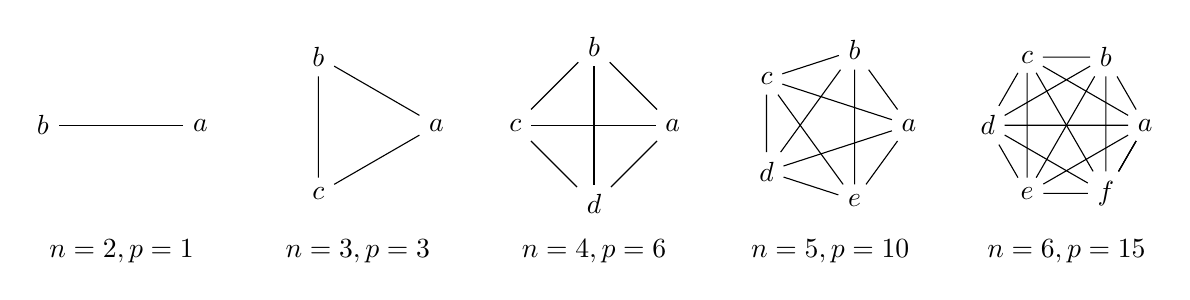
\begin{tikzpicture}[label distance=1.2cm]
\node (2) at (0,0) [label=below:{$n=2, p=1$}]{};
\node (3) at (3,0) [label=below:{$n=3, p=3$}]{};
\node (4) at (6,0) [label=below:{$n=4, p=6$}]{};
\node (5) at (9,0) [label=below:{$n=5, p=10$}]{};
\node (6) at (12,0)[label=below:{$n=6, p=15$}]{};
\path (2) ++(0:1)   node (a) {$a$};
\path (2) ++(180:1) node (b) {$b$};
\draw (a) -- (b);
\path (3) ++(0:1)   node (a) {$a$};
\path (3) ++(120:1) node (b) {$b$};
\path (3) ++(240:1) node (c) {$c$};
\draw (a) -- (b) -- (c) -- (a);
\path (4) ++(0:1)   node (a) {$a$};
\path (4) ++(90:1)  node (b) {$b$};
\path (4) ++(180:1) node (c) {$c$};
\path (4) ++(270:1) node (d) {$d$};
\draw (a) -- (b) -- (c) -- (d) -- (a) ;
\draw (a) -- (c)    (d) -- (b) ;
\path (5) ++(0:1)   node (a) {$a$};
\path (5) ++(72:1)  node (b) {$b$};
\path (5) ++(144:1) node (c) {$c$};
\path (5) ++(216:1) node (d) {$d$};
\path (5) ++(288:1) node (e) {$e$};
\draw (a) -- (b) -- (c) -- (d) -- (e) -- (a) ;
\draw (a) -- (c)    (d) -- (b)    (a) -- (d) ;
\draw (e) -- (b)    (e) -- (c) ;
\path (6) ++(0:1)   node (a) {$a$};
\path (6) ++(60:1)  node (b) {$b$};
\path (6) ++(120:1) node (c) {$c$};
\path (6) ++(180:1) node (d) {$d$};
\path (6) ++(240:1) node (e) {$e$};
\path (6) ++(300:1) node (f) {$f$};
\draw (a) -- (b) -- (c) -- (d) -- (e) -- (f) -- (a) ;
\draw (a) -- (c)    (d) -- (b)    (a) -- (d) ;
\draw (e) -- (b)    (e) -- (c)    (a) -- (f) ;
\draw (d) -- (f)    (b) -- (f)    (a) -- (f) ;
\draw (c) -- (f)    (a) -- (e) ;
\end{tikzpicture}

The basic idea  behind the $t$ test is to divide the difference between 
two values by a measure of how much uncertainty there is about the size 
of that difference. The measure of uncertainty used is the 
\emph{standard error}.

\[
	t=\frac{\textrm{difference between values}}{\textrm{standard error}}
\]

When there is no difference between the values $t$ will be zero, but 
with big differences and/or small errors, will be larger. The $t$ 
distribution below shows how commonly different values of $t$ are found 
under the null hypothesis. 
\begin{center}
\includegraphics[width=0.7\textwidth]{tvals.pdf} 
\end{center}
 
Some points about the plot above:
\begin{compactitem}
	\item The  null hypothesis is that there is no difference between the 
	values but because we only estimate the values from samples, 
	differences will creep in by chance.
	\item Mostly these differences will be small --- hence the peak in 
	the middle --- but sometimes the differences will be large and the 
	errors will be small.
	\item 95\% of the area under the curves are between these two sets of 
	vertical lines. Values of $t$ more extreme than this will only occur 
	1 in 20 times or with a probability ($p$) of 0.05.
	\item The means of small samples are more easily influenced by 
	extreme values and so produce extreme $t$ values more frequently. 
	This is why the red curve above for smaller samples is more flattened 
	out and why the 95\% limits are more spread out.
\end{compactitem}

\section{One sample $t$ tests}

In the simplest example, a $t$ test can be used to test whether the 
mean of a sample is different from a specific value. For example:

\begin{compactitem}
	\item Is the ozone in a set of air samples above the legal limit?
	\item Is the change in a set of patient' weights different from zero?
	\item Is the mean genome size for Odonata smaller than 1.25 pg, which 
	is the average for insects 
	\href{http://www.genomesize.com/statistics.php?stats=insects}{[see 
	here]}?
\end{compactitem}

Oh look! We can test that last one\ldots 

To calculate $t$, we need that observed difference and then the 
standard error of the difference between the mean of our sample and the 
known value. This is calculated using the \emph{variance} and the 
\emph{sample size} ($n$) of the sample ($s$). 

\[se_s = \sqrt{\frac{\textrm{var}(s)}{n}}\]

This simple equation trades off variance --- high variance in the data 
gives higher uncertainty about the location of the mean --- and sample 
size -- more data gives more certainty. So, \emph{low variance} and 
\emph{large datasets} have \emph{small} standard errors; \emph{high 
variance} and \emph{small datasets} have \emph{large} standard errors. 
Variance is calculated using sums of squares and so the square root is 
needed to give a standard error in the same units as the mean.  

So, all we need are three values calculated from the data: mean, 
variance and the number of data points and we can calculate $t$. R can 
do this for us:

\begin{lstlisting}
# calculate the three values from the data:
> mean.gs <- mean(genome$GenomeSize)
> print(mean.gs)
[1] 1.014
> var.gs <- var(genome$GenomeSize)
> print(var.gs)
[1] 0.1397
> n.gs <- length(genome$GenomeSize)
> print(n.gs)
[1] 100
# get the difference
> diff <- mean.gs - 1.25
> print(diff)
[1] -0.2357
# get the standard error
> se.gs <- sqrt(var.gs/n.gs)
> print(se.gs)
[1] 0.03738
# get the t value
> t.gs <- diff/se.gs
> print(t.gs)
[1] -6.306
\end{lstlisting}

\begin{compactitem}[$\quad\star$]
\item Copy and paste the code above into your script in R and run it. 
Read through the code and make sure you understand the steps.
\end{compactitem}

This is a big $t$ value --- values this extreme don't even appear on 
the graph above --- so we would conclude that the mean genome size for 
Odonata is different from the average for insects.

We can do this more easily and get some more information using the 
function {\tt t.test}. The null hypothesis can be set using the option 
(sometimes called a function \emph{argument}) {\tt mu} --- the Greek 
letter $\mu$ is often used to refer to a mean:

\begin{lstlisting}
> t.test(genome$GenomeSize, mu = 1.25)
 
	One Sample t-test
 
 data:  genome$GenomeSize 
 t = -6.306, df = 99, p-value = 8.034e-09
 alternative hypothesis: true mean is not equal to 1.25 
 95 percent confidence interval:
  0.9401 1.0885 
 sample estimates:
 mean of x 
     1.014 
\end{lstlisting}

This confirms the values we calculated by hand and adds a $p$ value. 
The output also gives the degrees of freedom. This is something we will 
come back to later, but the degrees of freedom are basically the number 
of data points minus the number of estimated parameters, which in this 
case is one mean.

The output also gives a confidence interval for the observed mean. 
The mean is the best estimate of the population mean given our sample 
of species of Odonata, but the actual mean for the order could be 
bigger or smaller. The confidence interval tells us the region in which 
we are 95\% confident that this actual mean lies.
 
It is calculated using the $t$ distribution. Remember that $t$ is a 
difference divided by a standard error; if we multiply $t$ by a 
standard error, we get back to a difference. If we pick a pair of $t$ 
values that contain the middle 95\% of the $t$ distribution, as in the 
plot on page 2, then we can multiply that by the standard error from 
the data to get a range above and below the mean.  If we sampled lots 
of sets of 100 species of Odonata, we expect 95\% of the observed means 
to lie inside this range. The code below shows the calculation of the 
confidence interval for the test above.

\begin{lstlisting}
# Find the edges of the middle 95% of a t distribution with 99 df
# (quantiles of the t distribution, so qt)
> tlim <- qt(c(0.025,0.975), df = 99)
> print(tlim)
[1] -1.984 1.984
# use the mean and standard error from above to get a confidence interval
> mean.gs + tlim * se.gs
[1] 0.9401 1.0885
\end{lstlisting}

\begin{compactitem}[$\quad\star$]

	\item Using the {\tt t.test} code above as an template, test whether 
	the body weight (in grams) of Odonata is different from the 
	average\footnote{This slightly dodgy estimate comes from an estimated 
	average volume for arthropods of of 45.21 mm$^3$ and assuming a 
	density of 1 gm per cm$^3$. The volume is from: Orme, C. D. L., 
	Quicke, D. L. J., Cook, J. M. and Purvis, A. (2002), Body size does 
	not predict species richness among the metazoan phyla. Journal of 
	Evolutionary Biology, 15: 235--247.} for arthropods of 0.045 grams.

\end{compactitem}	

\section{Two sample $t$ tests}

It is more common to use a $t$ test to compare the means of two 
samples. This includes questions like:

\begin{compactitem}
	\item Do two rivers have the same concentration of a pollutant?
	\item Do chemical A and chemical B cause different rates of mutation?
	\item Do damselflies and dragonflies have different genome sizes?
\end{compactitem}

The main difference here is that with a one sample $t$ test, we assume 
that one of the means is known exactly: the only error is in the single 
sample. With a two sample test, we are comparing two means estimated 
from samples and both contain error. The graph below illustrates this:
\begin{center}
\includegraphics[width=0.9\textwidth]{twosampleIllustration.pdf} 
\end{center}
	
The vertical lines show the mean (solid lines) and one standard error 
to each side (dashed lines). The red mean is the same in both cases, 
but the second graph shows that this is also estimated from a sample 
with error: the difference in the means looks less convincing and we'd 
expect a smaller $t$ value. The $t$ tests in for these two graphs 
confirm this:

\begin{compactitem}
\item The mean for blue is significantly different from 16.74 
(mean=14.98, se=0.38, df=59, $t$=-4.65, $p$=0.00002). 
\item The means of blue and red are significantly different (blue: 
mean=14.98, se=0.38; red: mean=16.74, se=0.42; df=118, $t$=-3.13, 
$p$=0.002)
\end{compactitem}

\begin{compactitem}[$\quad\star$]
\item Have a close look at the previous two statements. This shows the 
kind of detail needed when reporting the results of $t$ tests. The 
following is \emph{not} acceptable: The means of blue and red are 
significantly different ($p=0.002$).
\end{compactitem}

So, with two samples, we shouldn't be so confident about the difference 
between the values --- it should have a higher standard error. We can 
do this simply by combining the variance and sample size for the two 
samples ($a$ and $b$) into the calculation:

\[
se_{a-b}= \sqrt{\frac{\textrm{var}(a)}{n_a} + \frac{\textrm{var}(b)}{n_b}}
\]

We'll use a $t$ test to address that last question: are the genome 
sizes of Anisoptera and Zygoptera different? First, we'll do this by 
hand. We'll use a really handy function {\tt tapply(X, INDEX, FUN)} to 
quickly find the values for the two groups: it takes some values (X), 
splits those values into groups based on a factor (INDEX) and runs each 
group through another function (FUN). 

\begin{lstlisting}
# calculate the three values from the data
> mean.gs <- tapply(X = genome$GenomeSize, INDEX = genome$Suborder, FUN = mean)
> print(mean.gs)
Anisoptera 	Zygoptera
1.018				1.012
> var.gs <- tapply(X = genome$GenomeSize, INDEX = genome$Suborder, FUN = var)
> print(var.gs)
Anisoptera 	Zygoptera
0.18458 		0.06946
> n.gs <- tapply(X = genome$GenomeSize, INDEX = genome$Suborder, FUN = length)
> print(n.gs)
Anisoptera 	Zygoptera
38					62

# get the difference
> diff <- mean.gs[1] - mean.gs[2]
> print(diff)
Anisoptera
-0.006647

# get the standard error of the difference
> se.gs <- sqrt((var.gs[1]/n.gs[1]) + (var.gs[2]/n.gs[2]))
> print(se.gs)
Anisoptera
0.06932

# get the t value
> t.gs <- diff/se.gs
> print(t.gs)
Anisoptera

-0.09589

\end{lstlisting}
 
\begin{compactitem}[$\quad\star$]
\item Type the code above into your script in R and run it. Again, read 
through the code and make sure you understand the steps.
\end{compactitem}

The {\tt t.test} function automates this all for us, and we can use a 
formula (see Chapter \ref{ch:ExpDesign}) to get a test between the two 
suborders.

\begin{lstlisting}
>  t.test(GenomeSize ~ Suborder, data = genome)
 
 	Welch Two Sample t-test
 
 data:  GenomeSize by Suborder 
 t = -0.0959, df = 98, p-value = 0.9238
 alternative hypothesis: true difference in means is not equal to 0 
 95 percent confidence interval:
  -0.1442  0.1309 
 sample estimates:
 mean in group Anisoptera  mean in group Zygoptera 
                    1.012                    1.018 
 
\end{lstlisting}
 
The output looks very similar to the one sample test, except that the 
output  now gives two estimated means, rather than one and it reports 
the $p$ value for the calculated $t$ value.

\begin{compactitem}[$\quad\star$]
\item Add this to your script and run it.
\item Copy and modify this in your script to test whether the body 
weight of the two suborders are different.
\end{compactitem}

\section{$F$ tests for equal variance}

$F$ tests are used to compare the variances of two samples or 
populations. You will most prominently see them in analysis of variance 
(ANOVA), to test the hypothesis that the means of a given set of 
normally distributed populations all have the same variance. 

Let's use our genomesize datast to have a look at F-tests as well. 
Ideally, the $t$ test should be used with data that are: i) 
\emph{relatively normally distributed}, so that means can be estimated 
sensibly; and ii) have \emph{similar variances}. We'll deal with the 
similar variance question here using an $F$ test for equal variances. 

First, let's visualize the data. As I hope you've already noticed, this 
session has been neglecting one very important part of analysis --- 
\emph{plotting the data}. We are going to compare two plots, so it 
helps to have them side by side in the same window. We can use the 
function {\tt par} to change a set of options called graphics 
parameters to get R to do this. The option to change is {\tt mfrow}. 
This sets a graphics window to include \emph{m}ultiple \emph{f}igures 
and we need to tell R the number of rows and columns to divide the 
window into: {\tt par(mfrow=c(1,2))}.
  
\begin{compactitem}[$\quad\star$]
\item Copy {\tt par(mfrow=c(1,2))} into your script, add a comment and 
run it.
\item Using your (rapidly improving!) R skills, create a boxplot comparing the 
genome sizes of the two suborders.
\item Add another boxplot beside it comparing the body weight of the 
two suborders.
\end{compactitem}
It should look like this:
\begin{center}
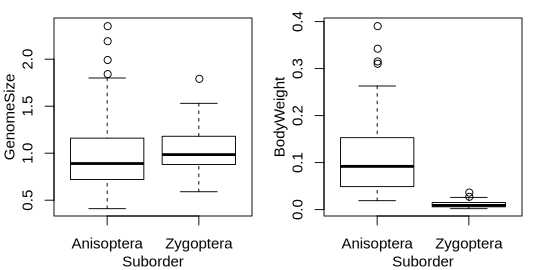
\includegraphics[width=0.9\textwidth]{bxp.pdf} 
\end{center}

The distribution of the test statistic $F$ is simply the ratio of the 
variances for sample $a$ and $b$: $\textrm{var}(a)/\textrm{var}(b)$. If 
the two variances are the same then $F=1$; if $\textrm{var}(a) > 
\textrm{var}(b)$ then $F > 1$; and if $\textrm{var}(a) < 
\textrm{var}(b)$ then $F < 1$ (\ref{fig:fdist}).

\begin{figure}
	\centering
	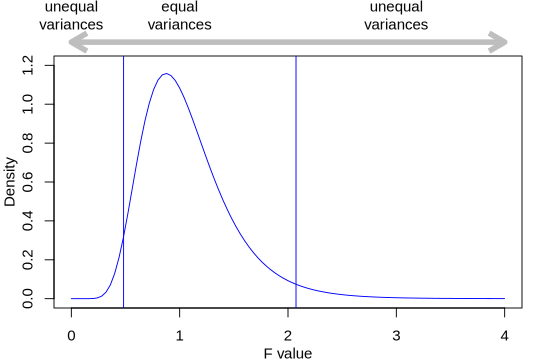
\includegraphics[width=0.7\textwidth]{fvals.pdf} 
	\caption[Caption for LOF]{The F distribution. The two vertical blue 
	lines show the edges of the central 95\% of the area of the curve: if 
	the two samples are drawn at random from a population with the same 
	variance then values of $F < 0.482$ or $> 2.074$ are observed fewer 
	than 1 time in 20 ($p\le0.05$ )\protect\footnotemark . The shape of 
	the $F$ distribution changes depending on the amount of data in each 
	of the two samples but will always be centered 
	near 1 and with a tail to the right (right-skewed). Note that the 
	F-distribution arises as the ratio of two appropriately scaled {\it 
	chi-square distributed variates}, because, as we saw above, variances 
	should be chi-square distributed.}
\label{fig:fdist} 
\end{figure}
\footnote{Note that $1/0.482 \approx 2.074$ 
	and $1/2.074 \approx 0.482$: in this case, it doesn't matter which 
	way round you compare the two variances!}

We can use R to calculate $F$ for the variance in genome size in each 
of the two suborders. We calculated the variance for the $t$ test 
above, so we can just do this:

\begin{lstlisting}
> var.gs[1]/var.gs[2]
Anisoptera
		2.657
\end{lstlisting}

That's quite a big $F$ value and we can use the function {\tt var.test} 
to do all the calculations for us and give us the actual $p$ value:

\begin{lstlisting}
> var.test(GenomeSize ~ Suborder, data = genome) 
 	F test to compare two variances
 
 data:  GenomeSize by Suborder 
 F = 2.657, num df = 61, denom df = 37, p-value = 0.001946
 alternative hypothesis: true ratio of variances is not equal to 1 
 95 percent confidence interval:
  1.449 4.671 
 sample estimates:
 ratio of variances 
              2.657 
\end{lstlisting}

It produces the same value that we calculated by hand and shows that, 
if the two samples are drawn from populations with the same variance,  
an $F$ value this extreme will only be observed roughly 1 time in 500 
($1/0.00195 \approx 500$) .
 
\begin{compactitem}[$\quad\star$]
\item Open a new empty script called {\tt FTests.R}.
\item In this write your script to test whether the variances in the 
body weight of the two suborders from the {\tt GenomSize} dataset are 
different.
\end{compactitem}
 
There are clearly problems with the variance in both examples. The next 
two sections present ways to address these kinds of problems.

\section{$t$ tests revisited}

The first thing to say is that R is aware of the problem with the 
variance. If you look back at the output from the previous $t$ tests, 
you will see that the degrees of freedom vary a lot. We have 100 
observations and -- after subtracting one for each mean we calculate 
--- our degrees of freedom should be either 99 (one sample test) or 98 
(two sample test). What we actually see are smaller numbers, with the 
smallest being {\tt df = 60.503} for the two sample test of body 
weight. 

 
The explanation is that R is applying a \emph{penalty} to the degrees 
of freedom to account for differences in variance. With fewer degrees 
for freedom, more extreme $t$ values are more likely and so it is 
harder to find significant results. This doesn't mean we can forget 
about checking the variances or plotting the data!

In this case, we can also apply a transformation to the data in order 
to make the variances more equal. Forgetting the wings and assuming 
Odonata are shaped like a box, the model in the graph below shows how 
volume changes with length: equal changes in length do not lead to 
equal changes in volume and longer species will have a 
disproportionately large volume. This is a classic feature of 
morphological data known as allometric scaling and we'll look at it 
again in Chapter \ref{ch:ANOVA}. In the meantime, a log transformation will 
turn body weight from a skewed distribution to a more normal 
distribution.
 
\begin{center}
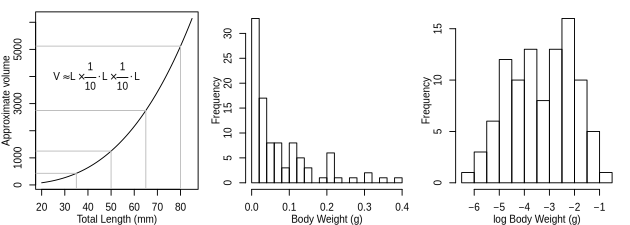
\includegraphics[width=\textwidth]{transform.pdf} 
\end{center}

% We can create a new variable in the {\tt genome} data frame of 
$\log_e$ body weight as follows:

\begin{lstlisting}
> genome$logBodyWeight <- log(genome$BodyWeight)
\end{lstlisting}


\begin{compactitem}[$\quad\star$]
\item Copy the line into your script and run it.
\item Now write three lines of code to get a boxplot of $\log_e$ body 
weight and then run a variance test and $t$ test on the differences in 
$\log_e$ body weight between suborders.
\end{compactitem}

This gives a much clearer result --- the variances are almost identical 
and the differences between the suborders are much more cleanly tested.

 
\section{Non-parametric tests}

What happens if there isn't a convenient transformation for the 
variable that gives roughly constant variation and equal variance?  In 
a parametric test, like the $t$ and $F$ test above, we use parameters 
(mean and variance) to describe the data, assume these describe the 
data well and then just use these parameters to run the test. If these 
assumptions don't seem very sound, the non-parametric tests provide a 
way of using the ranks of the data to test for differences. They aren't 
as powerful --- they are less likely to reveal significant differences 
--- but they are more robust. The most commonly used alternative is the 
Wilcoxon test, which uses the function {\tt wilcox.test} in R.

\begin{compactitem}[$\quad\star$]

\item Using {\tt wilcox.test} as a replacement for {\tt t.test}, repeat 
the one and two sample $t$ test for genome size and body weight.
\item Compare the two results.
\item Repeat the same with the predator and prey body mass data from 
the plotting and visualization chapter in SilBioComp.pdf -- check how 
different the results are when using $t$ vs. Wilcoxon test.

\end{compactitem}
 % t_F_tests}
\chapter{Linear Models: Regression}
\label{ch:regress}

Aims of this chapter\footnote{Here you work with the script file {\tt regress.R}}:

\begin{compactitem}
	\item More functions for plotting data and models.
	\item Calculating correlation coefficients.
	\item Fitting a regression model and significance testing.
	\item Using diagnostic plots to assess model suitability.
\end{compactitem}

As with the previous chapter, we'll start with creating a new blank 
script for you to fill in during the practical. We'll also be using the 
genome size data again, so:

\begin{compactitem}[$\quad\star$]
	\item Open R and change to the {\tt code} directory.
	\item Create a new blank script called `Regression.R' and add some 
	introductory comments.
	\item Add code to your script to load the genome size data into R and 
	check it.
\end{compactitem}

\section{Exploring the data}

In previous chapters we used {\tt plot} to create a scatterplot between 
two variables. If you have a set of variables to explore, writing code 
for each plot is tiresome, so R provides a the function {\tt pairs}, 
which creates a grid of scatterplots between each pair of variables. 
All it needs is a dataset.

\begin{compactitem}[$\quad\star$]
	\item Add {\tt pairs(genome, col=genome\$Suborder)} into your script 
	and run the code. 
\end{compactitem}

The result is messy! There are far too many variables in {\tt genome} 
for this to be useful. We need to cut down the data to fewer variables. 
In Chapter \ref{ch:ExpDesign}, we used indices to select colours; here, we can use 
indices to select columns from the data frame. This again uses square 
brackets ({\tt x[ ]}), but a data frame has two dimensions, rows and 
columns, so  you need to provide an index for each dimension, separated 
by commas. If an index is left blank, then all of that dimension (i.e. 
all rows or columns) are selected. Try the following to re-acquaint 
yourself to access data frame content using indices:  

\begin{lstlisting}
# create a small data frame:
> dat <- data.frame(A = c("a", "b", "c", "d", "e"), B = c(1, 2, 3, 4, 5))
> dat[1, ] # select row 1 (all columns selected)
	A B
1 a 1

> dat[, 2] # select column 2 (all rows selected)
[1] 1 2 3 4 5
> dat[2, 1] # select row 2, column 1
[1] "b"

\end{lstlisting}

Now let's get started with the actual analysis. We will look at five 
key variables: genome size, body weight, total length, forewing length 
and forewing area. If you look at the output of {\tt str(genome)}, 
you'll see that these are in columns 4, 7, 8, 12 and 14. We can record 
the indices of these columns and use this to select the data in the 
pairs plot.

\begin{lstlisting}
morpho <- c(4, 7, 8, 12, 14)
pairs(genome[, morpho], col = genome$Suborder)	
\end{lstlisting}

\begin{compactitem}[$\quad\star$]
	\item Add the code above to your script and run it
\end{compactitem}

The {\tt pairs} plot should give you something like the plot below:

\begin{center}
	\includegraphics[width=\textwidth]{pairs.pdf} 
\end{center}

Each scatterplot is shown twice, with the variables swapping between 
the $x$ and $y$ axes. You can see immediately that the relationships 
between the four morphological measurements and genome size are fairly 
scattered but that the plots comparing morphology show much clearer 
relationships.

\section{Correlations}

One way of summarising how close strong the relationship between these 
variables are is to calculate a correlation coefficient. Pearson 
correlations look at the difference of each point from the mean of each 
variable (and since it uses means, it is a parametric statistic). 

It is calculated using of the differences from the mean on each axis. 
The key calculation is --- for each point -- to get the product of the 
differences on each axis and add them up. If the points are mostly top 
left ($-x$, $y$) or bottom right ($x$, $-y$) then these products are 
mostly negative ($-xy$); if the points are mostly top right ($x$, $y$) 
or bottom left ($-x$, $-y$) then the products are mostly positive 
($xy$).  

\begin{center}
	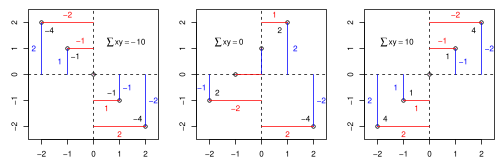
\includegraphics[width=\textwidth]{corr.pdf} 
\end{center}

The plots above show three clear cases where all the values of $xy$ are 
negative or positive or where both are present and sum to zero. The 
Pearson correlation coefficient simply scales these sums of $xy$ to be 
between -1 (perfectly negatively correlated) and 1 (perfectly 
positively  correlated) via zero (no correlation).

We will use two functions to look at correlations. The first is {\tt 
cor}, which can calculate correlations between pairs of variables, so 
is a good partner for {\tt pairs} plots. The second is {\tt cor.test}, 
which can only compare a single pair of variables, but uses a $t$ test 
to assess whether the correlation is significant. 

\begin{compactitem}[$\quad\star$]
	\item Try the following (and include it in your R script file)
\end{compactitem}


\begin{lstlisting}
> cor(genome[, morpho], use = "pairwise")
\end{lstlisting}

You should see a correlation matrix. Then,

\begin{lstlisting}
> cor.test(genome$GenomeSize, genome$TotalLength, use = "pairwise")	

Pearson's product-moment correlation

data: genome$GenomeSize and genome$TotalLength
t = 3.551, df = 96, p-value = 0.0005972

alternative hypothesis: true correlation is not equal to 0 
95 percent confidence interval:
  0.1526 0.5050 
sample estimates:
    cor 
 0.3407   
\end{lstlisting}

The {\tt use='pairwise'} in the above tells R to omit observations with 
missing data and use complete pairs of observations. The first function 
confirms our impressions from the graphs: the correlations between 
genome size and morphology are positive but comparatively weak and the 
correlations between morphological measurements are positive and very 
strong (i.e. close to 1). The correlation test tells us that genome 
size and body length are positively correlated (r=0.34, $t$ = 3.5507, 
df = 96, $p$ = 0.0006).

\begin{compactitem}[$\quad\star$]
	\item Again, remember this example when reporting correlations!
\end{compactitem}

\section{Transformations and allometric scaling}

There is one problem with the correlations above: {\it correlations 
assume a straight line relationship}. Some of the scatterplots above 
are fairly straight but there are some strongly curved relationships. 
This is due to the allometric scaling mentioned in Chapter \ref{ch:ExpDesign}: two of 
the variables are in linear units (total and forewing length), one is 
in squared units (forewing area) and one in cubic units (body weight, 
which is approximately volume).

The relationships between these variables can be described using a 
power law: $y = ax^b$. Fortunately, if we log transform this equation, 
we get $\log(y) = \log(a) + b \log(x)$. This is the equation of a 
straight line ($y=a+bx$), so we should be able to make these plots 
straighter by logging both axes. We saw in Chapter \ref{ch:ExpDesign} that we can 
create a new logged variable in the data frame like this:

\begin{lstlisting}
> genome$logGS <- log(genome$GenomeSize)
\end{lstlisting}

\begin{compactitem}[$\quad\star$]
	\item Using this line as a template, create a new logged version of 
	the five variables listed above.
	\item Using {\tt str}, work out which column numbers the logged 
	variables are and create a new variable called {\tt logmorpho} 
	containing these numbers.
	\item Copy the {\tt pairs} and {\tt cor} test from earlier in your 
	script and modify them to run these functions for the columns given 
	in {\tt logmorpho}.
\end{compactitem}

The correlations should give the following output:
\begin{lstlisting}
> cor(genome[, logmorpho], use = "pairwise")

         logGS   logBW  logTL  logFL   logFA
 logGS 1.00000 0.08406 0.2224 0.1150 0.06808
 logBW 0.08406 1.00000 0.8892 0.9456 0.94996
 logTL 0.22244 0.88919 1.0000 0.9158 0.86207
 logFL 0.11500 0.94565 0.9158 1.0000 0.97916
 logFA 0.06808 0.94996 0.8621 0.9792 1.00000
\end{lstlisting}

The scatterplots should look like this and show that logging the data 
has very successfully removed allometric scaling effects in the data:
\begin{center}
\includegraphics[width=\textwidth]{pairsLog.pdf} 
\end{center}

\section{Regression}

We'll now look at fitting the first linear model of this course, to 
explore whether log genome size explain log body weight. The first 
thing to do is to plot the data:

\begin{center}
	\includegraphics[width=0.5\textwidth]{gsVbw.pdf} 
\end{center}

It is clear that the two suborders have very different relationships: 
to begin with we will look at dragonflies (Anisoptera). We will 
calculate two linear models:

\begin{compactdesc}
	\item [The null model] This is the simplest linear model: nothing is 
	going on and the response variable just has variation around the 
	mean: $y = \beta_1$. This is written as an R formula as {\tt y 
	\textasciitilde{} 1}.
	\item [Linear regression] This models a straight line relationship 
	between the response variable and a continuous explanatory variable: 
	$y= \beta_1 + \beta_{2}x$.
\end{compactdesc}

The code below fits these two models.

\begin{lstlisting}
> nullModelDragon <- lm(logBW ~ 1, data = genome, subset = Suborder == 
"Anisoptera")
> genomeSizeModelDragon <- lm(logBW ~ logGS, data = genome, subset = 
Suborder == "Anisoptera")
\end{lstlisting}

\begin{compactitem}[$\quad\star$]
	\item Note the long names for the models. Short names are easier to 
	type but calling R objects names like {\tt mod1},  {\tt mod2},  {\tt 
	xxx} swiftly get confusing!   
	\item Enter these models into your script and run them.
\end{compactitem}

Now we want to look at the output of the model. Remember from the 
lecture that a model has {\it coefficients} (the $\beta$ values in the 
equation of the model) and {\it terms} which are the explanatory 
variables in the model. We'll look at the {\it coefficients} first:

\begin{lstlisting}
> summary(genomeSizeModelDragon) 
 Call:
 lm(formula = logBW ~ logGS, data = genome, subset = Suborder == 
     "Anisoptera")
 
 Residuals:
    Min     1Q Median     3Q    Max 
 -1.324 -0.612  0.097  0.519  1.324 
 
 Coefficients:
             Estimate Std. Error t value Pr(>|t|)    
 (Intercept)  -2.3995     0.0908  -26.41  < 2e-16 ***
 logGS         1.0052     0.2398    4.19  9.5e-05 ***
 ---
 Signif. codes:  0 '***' 0.001 '**' 0.01 '*' 0.05 '.' 0.1 ' ' 1 
 
 Residual standard error: 0.697 on 58 degrees of freedom
   (2 observations deleted due to missingness)
 Multiple R-squared: 0.233,	Adjusted R-squared: 0.219 
 F-statistic: 17.6 on 1 and 58 DF,  p-value: 9.54e-05  
\end{lstlisting}

There is a lot of information there: the model description (`{\tt 
Call}'), a summary of the residuals, a table of coefficients and then 
information on residual standard error, r squared and an $F$ test. All 
of these will become clearer during this course --- for the moment, 
concentrate on the coefficients table.

There are two rows in the coefficient table, one for each coefficient 
in $y=\beta_1 + \beta_2x$ --- these are the intercept and the slope of 
the line. The rest the details on each row are a $t$ test  of whether 
the slope and intercept are significantly different from zero. 

Now we will look at the {\it terms} of the model using the {\tt anova} 
function. We will have a proper look at ANOVA (Analysis of Variance) in 
chapter \ref{ch:ANOVA}. Meanwhile, for our current purposes, all you need to 
know is that ANOVA tests how much variation in the response variable is 
explained by each explanatory variable. We only have one variable and 
so there is only one row in the output:

\begin{lstlisting}
> anova(genomeSizeModelDragon)

 Analysis of Variance Table
 
 Response: logBW
           Df Sum Sq Mean Sq F value  Pr(>F)    
 logGS      1   8.53    8.53    17.6 9.5e-05 ***
 Residuals 58  28.14    0.49                    
 ---
 Signif. codes:  0 '***' 0.001 '**' 0.01 '*' 0.05 '.' 0.1 ' ' 1 
\end{lstlisting}

This table is comparing the variation in log body weight explained by 
log genome size to the total variation in log body weight. We are 
interested in how much smaller the residuals are for the genome size 
model than the null model. Graphically, how much shorter are the red 
residuals than the blue residuals:

\begin{center}
\includegraphics[width=0.8\textwidth]{regResid.pdf} 
\end{center}

We can get the sums of the squares of these residuals from the two 
models using the function {\tt resid}, and then square them and add 
them up:

\begin{lstlisting}
> sum(resid(nullModelDragon) ^ 2)
 [1] 36.67
 
> sum(resid(genomeSizeModelDragon) ^ 2)
 [1] 28.14
\end{lstlisting}

So we have five columns in the table:
\begin{compactdesc}
	\item[Df] This shows the degrees of freedom. Each fitted parameter/coefficient takes up 
	a degree of freedom from the total sample size, and the left over are the residuals degree of freedom. In this 
	case, genome size adds a slope (compare the null model $y=\beta_1$ 
	and this model $y=\beta_1 + \beta_2x$ --- there is one more $\beta$). 
	\item[Sum Sq] This shows sums of squares. The bottom line is the 
	residual sum of squares for the model and the one above is the 
	variation explained by genome size. Using the two values from above, 
	the sums of square residuals for the null model are 36.67. In the 
	genome size model, the sum of square residuals are 28.14 and so 
	$36.67-28.14=8.53$ units of variance have been explained by this 
	model.
	\item[Mean Sq] These are just the Sum Sq (Sum of Squares) values divided by the 
	degrees of freedom. The idea behind this is simple: if we explain 
	lots of variation with one coefficient, that is good (the null model), and if we explain a 
	small amount of variation with a loss of degree of freedom (by adding and then estimating more parameters), then that is bad.
	\item[F value] This is the ratio of the Mean Sq for the variable and 
	the residual Mean Sq. This is used to test whether the explained 
	variation is large or small.
	\item[Pr(>F)] This is a $p$ value --- the probability of the variable 
	explaining this much variance by chance. 
\end{compactdesc}

In this case, it is clear that genome size explains a significant 
variation in body weight. 

\begin{compactitem}[$\quad\star$]
	\item Include the {\tt summary} and {\tt anova} commands for {\tt 
	genomeSizeModelDragon} in your script, run them and check you are 
	happy with the output.
	\item Using this code as a template, create a new model called {\tt 
	genomeSizeModelDamsel} that fits log body weight as a function of log 
	genome size for damselflies.
	\item Write and run code to get the  {\tt summary} and {\tt anova} 
	tables for this new model.
\end{compactitem}

\section{Plotting the model}

Now we can plot the data and add lines to show the models. For simple 
regression models, we can use the function {\tt abline(modelName)} to 
add a line based on the model.
\begin{compactitem}[$\quad\star$]
 \item You already know how to create and customise scatterplots from 
 previous chapters. Create a plot of log body weight as a function of 
 log genome size, picking your favourite colours for the points.
 \item Use {\tt abline} to add a line for each model and use the {\tt 
 col} option in the function to colour each line to match the points. 
 For example: {\tt abline(genomeSizeModelDragon, col='red')}.
\end{compactitem}

You should get something like Figure \ref{fig:GenoRegModels}.

\begin{figure} \centering
	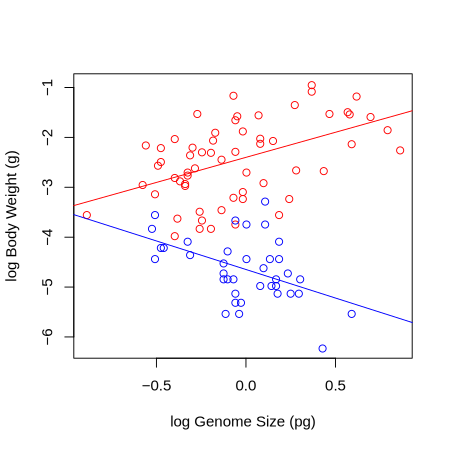
\includegraphics[width=0.5\textwidth]{GenoRegModels.pdf}
	\caption{Linear regression models fitted to the body weight vs. 
	genome size to the Dragonfly (red) and Damselfly (blue) subsets of 
	the data.}
	\label{fig:GenoRegModels}
\end{figure}

\section{Model diagnostics}

Now that we have our models, we need to check that they are appropriate 
for the data. For this, we will inspect ``diagnostic plots''. Producing 
diagnostic plots is easy in R --- if you {\tt plot} a model, then R 
produces a set of diagnostic plots! 

\begin{compactitem}[$\quad\star$]
	\item Try the following code (and include in the R script file):
\end{compactitem}
\begin{lstlisting}
> par(mfrow = c(2, 2), mar = c(5, 5, 1.5, 1.5))
> plot(genomeSizeModelDragon)
\end{lstlisting}
This should give the plots shown in figure \ref{fig:DiagModDragon}.
\begin{figure} \centering
	\includegraphics[width=0.7\textwidth]{DiagModDragon.pdf}
	\caption{Diagnostics for the {\tt lm} fit to the Dragonfly data 
	subset.}
	\label{fig:DiagModDragon} 
\end{figure}
And,
\begin{lstlisting}
> par(mfrow = c(2, 2), mar = c(5, 5, 1.5, 1.5))
> plot(genomeSizeModelDamsel)
\end{lstlisting}
This should give the plots shown in figure \ref{fig:DiagModDamsel}.

\begin{figure}\centering
	\includegraphics[width=0.7\textwidth]{DiagModDamsel.pdf}
	\caption{Diagnostics for the {\tt lm} fit to the Damselfly data 
	subset.}
	\label{fig:DiagModDamsel} 
\end{figure}

The diagnostic plots are:
\begin{compactdesc}
		
		\item[Residuals vs Fitted] This plot is used to spot if the 
		distribution of the residuals (the vertical distance from a point 
		to the regression line) has {\it similar variance} for different 
		predicted values (the y-value on the line corresponding to each 
		x-value). There should be no obvious patterns (such as curves) or 
		big gaps. If there was no scatter, if all the points fell exactly 
		on the line, then all of the dots on this plot would lie on the 
		gray horizontal dashed line. The red line is a smoothed curve to 
		make it easier to see trends in the residuals. It is flat in the 
		Dragonfly model fit (Figure \ref{fig:DiagModDragon}), and a bit 
		more wavy than we would like in the in the Damselfly model fit 
		(Figure \ref{fig:DiagModDamsel}), but there are no clear trends in 
		either, which is what you hope to see. 
		
		\item[Normal Q--Q] This plot is to check whether the residuals are 
		{\it normally distributed } --- are the values of the observed 
		residuals similar to those expected under a normal distribution? 
		Ideally, the points should form a perfectly straight line, 
		indicating that the observed residuals exactly match the expected. 
		Here, note that the points lie pretty close to the dashed line in 
		both Figures \ref{fig:DiagModDragon} \& \ref{fig:DiagModDamsel}, 
		but deviate at the ends, especially for Damselflies. However, some 
		deviation is to be expected near the ends --- here these deviations 
		are just about acceptable.

		\item[Scale--Location] The x-axis on this plot is identical to the 
		Residuals vs Fitted plot -- these are the fitted values. The y-axis 
		is the square root of the {\it standardized residuals}, which are 
		residuals rescaled so that they have a mean of zero and a variance 
		of one. As a result, all y-axis values are positive. Thus large 
		residuals (both positive and negative) plot at the top, and small 
		residuals plot at the bottom (so only their {\it scale} is 
		retained). Thus, all of the numbered points (which will be the same 
		in all plots) plot at the top here. The red line here shows the 
		trend, just like the Residuals vs Fitted plot. The regression 
		analysis has assumed homoscedasticity, that the variance in the 
		residuals doesn't change as a function of the predictor. If that 
		assumption is correct, the red line should be relatively flat. It 
		is not quite as flat as we would like, especially for the Dragonfly 
		analysis (Figure \ref{fig:DiagModDragon}).
		
		\item[Residuals vs Leverage] This plot shows the standardized 
		residuals against leverage. ``Leverage'' is a measure of how much 
		each data point influences the linear model's coefficient 
		estimates. Because the regression line must pass through the 
		centroid (``pivot point'') of the data (Figure \ref{fig:Leverage}), 
		points that lie far from the centroid have greater leverage, and 
		their leverage increases if there are fewer points nearby. There 
		are two key things to note about this plot:
		\begin{figure} \centering
			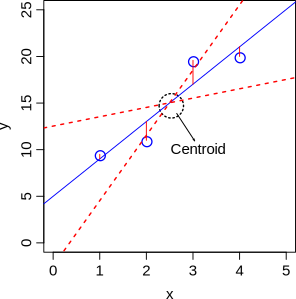
\includegraphics[width=0.4\textwidth]{Leverage.pdf}
			\caption{Leverage of data points on slope of a regression. The 
			points further away from the centroid in the x-axis direction 
			have more leverage, and can therefore move the regression line up 
			or down (dashed red lines).}
			\label{fig:Leverage} 
		\end{figure}

		\begin{enumerate}
			\item The standardized residuals (y-axis) are centered around 
			zero and reach 2-3 standard deviations away from zero. They 
			should also lie symmetrically about zero, as would be expected 
			for a normal distribution. This is the case for the Damselfly 
			plot (Figure \ref{fig:DiagModDamsel}) , but not so much for the 
			Dragonfly plot Figure \ref{fig:DiagModDragon}. 
			\item The contours values show {\it Cook's distance} (only 
			visible in the Damsefly plot), which measures how much the 
			regression would change if a point was deleted. Cook's distance 
			is increased by leverage and by large residuals: a point far from 
			the centroid with a large residual can severely distort the 
			coefficient estimates from the regression. On this plot, you want to see that the red smoothed 
			line stays close to the horizontal gray dashed line and that no 
			points have a large Cook's distance (i.e, >0.5). Both are true 
			here.
		\end{enumerate}
		This is an important diagnostic plot in regression analyses in 
		particular because it tells you whether your estimate of the slope 
		coefficient in particular is strongly affected by certain data 
		points.  

\end{compactdesc}
Note that certain points are numbered in all the plots --- these are 
points to pay special attention to because they are {\it potential} 
outliers. The numbers correspnd to the row number for that dataset in 
your data frame. You can easily identify these points in your data plot 
(Figure \ref{fig:GenoRegModels}) because the order of the points along 
the fitted values axis (y-axis) in the diagnostic plot matches the 
order along the x-axis in the data plot. So, fo example here, in Figure 
\ref{fig:DiagModDragon}, the two numbered points (46, 10) near the 
bottom correspond in the data plot (Figure \ref{fig:GenoRegModels}) to 
the two red points near the center-left that lie farthest below the red 
line.

Thus, neither the Drangonfly nor the Damselfly diagnostic plots look 
perfect, but this level of deviation from assumptions of linear models 
is acceptable. The main worrying factors are that the QQ plot for 
Damselflies indicates the observed residuals are a bit more extreme 
than expected, and the Scale--Location plot for Dragonflies suggests 
some pattern in the standardized residuals wrt location of the fitted 
values.

\begin{compactitem}[$\quad\star$]
 \item Copy the code to create the diagnostic plots into your script to 
 keep a record of the code and run it.
\end{compactitem}

\section{Reporting the model}

Now we know that the models are appropriate and we have a plot, the 
last thing is to report the statistics. For the damselfly model, here 
is one summary that would do: log genome size explains significant 
variation in log body weight in dameselflies (F=10.5, df=1,36, p=0.0025) 
and shows that body weight decreases with genome size (intercept: 
-4.65,  se=0.09; slope: -1.14, se=0.35).
 % regress}
\chapter{Linear Models: Analysis of variance}
\label{ch:ANOVA}

Aims of this chapter \footnote{Here you work with the script file {\tt anova.R}}:
\begin{compactitem}
	\item Plotting boxplots and barplots using factors
	\item Fitting factors in linear models using analysis of variance
	\item Diagnostic plots for explanatory factors
	\item Exploring differences between levels of a factor
\end{compactitem}

\section{What is ANOVA?}

\begin{figure}
	\centering
	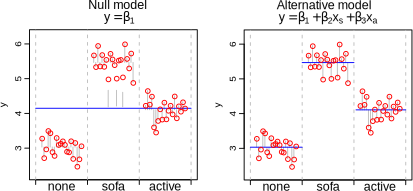
\includegraphics[width=.4\textwidth]{ANOVA_is_LM.pdf} 

	\caption{A dataset where an ANOVA would be appropriate. performing an 
	ANOVA test on this dataset is the same as fitting the linear model  
	$y  = \beta_1  + \beta_2 x_s + \beta_3 x_a$, where $x_s$ and $x_a$ 
	are two levels. There are three ``treatments'' here with the first 
	treatment, the control, captured by the baseline value $\beta_1$ 
	(the sample with the lowest value, on the far left)}

	\label{fig:anova1} 

\end{figure}

A {\it One-way analysis of variance} (one-way ANOVA) is a technique 
used to compare means of two or more samples representing numerical, 
continuous data. 

ANOVA tests the null hypothesis that samples from two or more groups 
are drawn from populations with the {\it same mean value}. To do this, 
ANOVA uses the {\it F}-statistic --- the ratio of the variance 
calculated across the samples (groups) (the null hypothesis) to the 
variance within the samples (groups). If the null hypothesis that the 
group means are drawn from populations with the same mean is indeed 
true, the between-group variance (numerator in the F-ratio) should be 
lower than the within-group variance (denominator). A higher ratio (and 
{\it F} value) therefore implies that the samples were drawn from 
populations with different mean values.

This is same as asking whether a linear model with a predictor (or 
explanatory variable) with at least two categorical levels (or 
factors), better accounts for the variance (Explained Sum of Squares, 
ESS) than a null model of the form $y  = \beta_1$ (Figure 
\ref{fig:anova1}). Thus, ANOVA is just a type of linear model. 

By the end of this chapter, it will make more sense to you how/why 
linear regression models that we covered in Chapter \ref{ch:regress}, 
of the form $y = \beta_1  + \beta_2 x$ (where $x$ is a continuous 
predictor variable),  require ANOVA to determine if the the model 
better fits than a null model of the form $y  = \beta_1$.

Typically, one-way ANOVA is used to test for differences among at least 
three groups, since the two-group (or levels or factors) case can be 
covered by a $t$-test (see Chapter~\ref{ch:t_F_tests}). When there 
are only two means to compare, the $t$-test and the F-test are 
equivalent; the relation between ANOVA and t is given by $F = t^2$. 

An extension of one-way ANOVA is two-way analysis of variance that 
examines the influence of two different categorical independent 
variables on one dependent variable --- we will look at multiple 
predictor variables in Chapter \ref{ch:MulExpl} onwards.

\section{Calculating the ANOVA test statistic}

ANOVA ``partitions'' variability in your data as follows: 

\begin{description}

	\item[Total sum of squares (TSS)] This is sum of the squared 
	difference between the observed dependent variable ($y$) and the mean 
	of the response variable $y$ (denoted by $\bar{y}$), i.e., 
	$$\text{TSS} = \sum_{i=1}^{n}(y_i - \bar{y})^2$$ TSS tells us how 
	much variation there is in the dependent variable without having any 
	other information (your null model). You might notice that TSS is the 
	numerator of the sample variance you learned about in Chapter 
	\ref{ch:ExpDesign}.
  
	\item [Explained sum of squares (ESS)] Sum of the squared differences 
	between the predicted $y$'s (denoted $\hat{y}$'s) and $\bar{y}$, or, 
	$$\text{ESS} = \sum_{i=1}^{n} (\hat{y}_i - \bar{y})^2$$ ESS tells us 
	how much of the variation in the dependent variable our alternative 
	(linear) model was able to explain. That is, it's the reduction in 
	uncertainty that occurs when the linear model is used to predict the 
	responses.
	
	\item [Residual sum of squares (RSS)] Sum of the squared differences 
	between the observed $y$'s (denoted by $y_i$) and the predicted 
	$\hat{y}$, or, $$\text{RSS} = \sum_{i=1}^{n} (\hat{y}_i - y_i)^2$$ 
	RSS tells us how much of the variation in the dependent variable our 
	model could not explain. That is, it's the uncertainty that remains 
	even after the linear model is used. The linear model is considered 
	to be statistically significant if it can account for a large amount 
	of variability in the response.

\end{description} 

And of course, TSS = ESS + RSS; the OLS method ``decomposes'' the total variation in the dependent variable into an explained component (ESS; explained by the predictor) and an unexplained or residual component (the RSS). 

These sums of squares can then be used to calculate the statistical 
significance of the linear model (Regression, ANOVA, etc) through the 
F-Value (or F-Ratio), as follows: 

\begin{center}
\def\arraystretch{1.5}
\begin{tabular}{|>{\centering}m{2cm}|>{\centering}m{2.1cm}|>{\centering}m{2cm}|>{\centering}m{2cm}|p{1.5cm}|}
\hline
Type of Sum of Squares (SS)  & Calculation & Degrees of Freedom (DF) & 
Mean Sum of Squares (MSS) & F-Value \\ \hline

TSS & $\sum_{i=1}^{n}(y_i - \bar{y})^2$   & $n-1$ &$\frac{TSS}{n-1}$& 
\multirow{3}{*}{ 
$\frac{\left(\frac{ESS}{n_c-1}\right)}{\left(\frac{RSS}{n-n_c}\right)}$} \\ \cline{1-4}

ESS & $\sum_{i=1}^{n} (\hat{y}_i - \bar{y})^2$ & $n_c-1$ & $\frac{ESS}{n_c-1}$ &  \\ \cline{1-4}

RSS & $\sum_{i=1}^{n} (\hat{y}_i - y_i)^2$ &  $n-n_c$ &  $\frac{RSS}{n-n_c}$ & \\ \hline
\end{tabular}
\end{center}

\subsection{Degrees of freedom}
Thus each sum of squares has a corresponding degrees of freedom (DF) 
associated with it that gives the Mean Sum of Squares (MSS)  --- the Sums of Squares divided by the corresponding degrees of freedom.

The TSS DF is one less than the number of observations $n-1$. This is because calculating TSS, needs $\bar y$ , which imposes loss of one degree of freedom. Note that MSS is thus nothing but the sample variance.

The ESS DF is one less than the number of coefficients ($n_c$) 
(estimated parameters) in the model: $n_c-1$. Note that in the case 
where the linear model is an ANOVA, it the number of coefficients 
equals the number of ``treatments'' (the categories or levels in the 
predictor). So for example, in Fig. \ref{fig:anova1}, there are three 
treatments (predictors) and therefore three coefficients ($\beta_1$, 
$\beta_2$, $\beta_3$), which means that the ESS degrees of freedom 
there is $n_c-1 = 2$. 

The RSS DF is the sample size $n$ minus the number of coefficients $n_c$, that is, $n - n_c$, because each estimated coefficient is an unknown parameter.

\subsection{The F-Value (or Ratio)}

Finally, The F-Value or F-Ratio, the test statistic used to decide 
whether the linear model fit is statistically significant, is the ratio 
of the Mean ESS to the Mean RSS. The null hypothesis is rejected if the 
F-ratio is large --- the model explains a significant amount of 
variance. The p-value is then calculated from the F-distribution as you 
learned before, in Chapter \ref{ch:t_F_tests} (see Fig. \ref{fig:fdist}).  

Also note that the Root Mean Square Error (RMSE), also known as the 
standard error of the estimate, is the square root of the Mean RSS. It 
is the standard deviation of the data about the Linear model, rather 
than about the sample mean.

\subsection{The $R^{2}$}

Finally, $R^{2}$, also called the Coefficient of Determination, is the 
proportion of total error (TSS) explained by the model (ESS), so the 
ratio ESS/TSS. That is it is the proportion of the variability in the 
response that is explained by  by the fitted model. Since TSS = ESS + 
RSS, $R^{2}$ can be rewritten as (TSS-RSS)/TSS = 1 - RSS/TSS. If a 
model has perfectly fits the data, $R^{2}=1$, and if it has no 
predictive capability $R^{2}=0$. In 
reality, $R^{2}$ will never be exactly 0 because even a null model will 
explain some variance just by chance due to sampling error. Note that 
$R$, the square root of $R^2$, is the multiple correlation coefficient: 
the correlation between the observed values ($y$), and the predicted 
values ($\hat{y}$).

As additional predictors (end therefore linear model coefficients) are 
added to a linear model, $R^2$ increases even when the new predictors 
add no real predictive capability. The adjusted-$R^2$ tries to addresses this 
problem of over-specification or over-fitting by including the degrees 
of freedom: Adjusted $R^2$ = 1 - (RSS/$n-n_c-2$)/(TSS/$n-1$) 
\footnote{That is, it is 1 minus the ratio of the square of the 
standard error of the estimate to the sample variance of the response}. 
Thus additional predictors with little explanatory capability will increase 
the ESS (and reduce the RSS), but they will also have lower RSS degrees of 
freedom (because of the additional number of fitted coefficients, 
$n_c$'s)\footnote{i.e., Standard error of the estimate won't 
decrease}. Thus if the additional predictors have poor predictive 
capability, these two reductions will cancel each other out. In other 
words, the Adjusted $R^2$ penalizes the addition of new predictors to 
the linear model, so you should always have a look at the Adjusted 
$R^2$ as a corrected measure of $R^2$.   

\section{A new dataset}

In this Chapter, we will use a new dataset of genome size and life 
history in mammals to try out a one-way ANOVA. The dataset is a 
composite of data taken from an online database of genome sizes and a 
published database of mammalian life history:

\begin{compactdesc}
	\item[Genome size] Average genome sizes for available mammal species 
	are taken from the online database  
	\href{www.genomesize.com}{www.genomesize.com}.
	\item[Life history] Trait data for these species are taken from: 
	\href{http://esapubs.org/archive/ecol/e090/184/metadata.htm}{
	Jones, K. E. {\it et al.} (2009) PanTHERIA: a species-level database 
	of life history, ecology, and geography of extant and recently 
	extinct mammals. Ecology 90, 2648--2648}.
\end{compactdesc}

\begin{compactitem}[$\quad\star$]
	\item Download the file {\tt MammalData.csv} from bitbucket and save 
	to your {\tt Data} directory.
	\item Create a new blank script called {\tt ANOVA\_Prac.R} and add 
	some introductory comments.
	\item Use {\tt read.csv} to load the data in the data frame 
	{\tt mammals} and then {\tt str} and {\tt summary} to examine 
	the data.
\end{compactitem}

There are nine variables. The first two are the latin binomial and 
taxonomic order of each species, followed by the species mean genome 
size (`C value', picograms), adult body mass (g), diet breadth, habitat 
breadth, litter size and then two factors showing whether the species 
are ground dwelling and their trophic level. For more information, see 
the link above.

You will see from the output of {\tt summary} that there is lots of 
missing data for the life history traits.

\section{Exploring the data with boxplots}

We are interested in finding out whether the mean C value for species 
varies predictably for different levels of life history traits (a 
typical one-way ANOVA question). For example: 

\begin{compactitem}
\item Do carnivores or herbivores have larger genome sizes?
\item Do ground dwelling mammals have larger or smaller genome sizes?
\end{compactitem}

Before we fit any models, we want to plot the data to see if the means 
within these groupings look different. We also want to check whether 
the variance looks similar for each group: {\it constant normal 
variance}! A simple way is to look at box and whisker plots, showing 
the median and range of the data:

\begin{compactitem}[$\quad\star$]
	\item Use {\tt plot(meanCvalue \textasciitilde{} TrophicLevel, 
	data= mammals)} to generate a boxplot of the differences in genome 
	sizes between trophic levels.
	\item Looking at the plots, it is clear that there is more spread in 
	the data above the median than below. Create a new variable {\tt 
	logCvalue} in the {\tt mammals} data frame containing logged C 
	values.
	\item Create a boxplot of log C values within trophic groups.
	\item Repeat the two plot commands to look at differences between 
	ground dwelling and other species.
\end{compactitem}

\section{Differences in means with barplots}

Box and whisker plots show the median and spread in the data very 
clearly, but we want to test whether the means are different. This is 
$t$ test territory --- how different are the means given the standard 
error --- so it is common to use barplots and standard error bars to 
show these differences.

We're going to use some R code to construct a barplot by hand. We need 
to calculate the means and standard errors within trophic groups, but 
before we can do that, we need a new functions to calculate the 
standard error of a mean:

\begin{lstlisting}
	
# get standard error of the mean from a set of values (x)

seMean <- function(x){
	x <- na.omit(x) # get rid of missing values

	se <- sqrt(var(x)/length(x)) # calculate the standard error

	return(se) 	# tell the function to return the standard error
}

\end{lstlisting}
	
Now we can use the function {\tt tapply}: it splits a variable up into 
groups from a factor and calculates statistics on each group using a 
function.
\begin{lstlisting}
trophMeans <- tapply(mammals$logCvalue, mammals$TrophicLevel, FUN = 
mean, na.rm = TRUE)

print(trophMeans)

 Carnivore Herbivore  Omnivore 
     1.085     1.197     1.236 
\end{lstlisting}

\begin{lstlisting}
trophSE <- tapply(mammals$logCvalue, mammals$TrophicLevel, FUN = seMean)

print(trophSE)

 Carnivore Herbivore  Omnivore 
   0.03983   0.02206   0.01844 
\end{lstlisting}

Now we have to put these values together on the plot:

\begin{lstlisting}
# get the upper and lower limits of the error bars
upperSE <- trophMeans + trophSE
lowerSE <- trophMeans - trophSE

# get a barplot
# - this function can report where the middle of the bars are on the x-axis
# - set the y axis limits to contain the error bars

barMids <- barplot(trophMeans, ylim=c(0, max(upperSE)), ylab = 'log C value (pg)')

# Now use the function to add error bars
# - draws arrows between the points (x0,y0) and (x1,y1)
# - arrow heads at each end (code=3) and at 90 degree angles

arrows(barMids, upperSE, barMids, lowerSE, ang=90, code=3)

\end{lstlisting}

\begin{center}
	\includegraphics[width=0.7\textwidth]{TLbarplot.pdf}
\end{center} 

Now we need to draw all these pieces together into a script and get 
used to using them.
\begin{compactitem}[$\quad\star$]
	\item Copy all the lines of code from this section into your script.
	\item Run it and check you get the graph above.
	\item Use the second two chunks as a model to plot a similar graph 
	for {\tt GroundDwelling}. You should get something like the plot 
	below.
\end{compactitem}

\begin{center}
	\includegraphics[width=0.6\textwidth]{GDbarplot.pdf}	
\end{center}
 
\section{An alternative to barplots}

That is a lot of work to go through for a plot. Doing it the hard way 
uses some useful tricks, but one strength of R is that there is a huge 
list of add-on packages that you can use to get new functions that 
other people have written.

We will use the {\tt gplots} package to create  plots of group means 
and confidence intervals. Rather than plotting the means $\pm$ 1 
standard error, the option {\tt p=0.95} uses the standard error and the 
number of data points to get 95\% confidence intervals. The default 
{\tt connect=TRUE} option adds a line connecting the means, which isn't 
useful here. 

\begin{compactitem}[$\quad\star$]
	\item Replicate the code below into your script and run it to get the 
	plots below.
\end{compactitem}

\begin{lstlisting}
#Load the gplots package
> library(gplots)

# Get plots of group means and standard errors
> par(mfrow=c(1,2))
> plotmeans(logCvalue ~ TrophicLevel, data=mammals, p=0.95, connect=FALSE)
> plotmeans(logCvalue ~ GroundDwelling, data=mammals, p=0.95, connect=FALSE)
\end{lstlisting}


\begin{center}
	\includegraphics[width = \textwidth]{test.pdf}	
\end{center}

\section{Analysis of variance}

Hopefully, those plots should convince you that there are differences 
in genome size between different trophic groups and between ground 
dwelling and other mammals. We'll now use a linear model to test 
whether those differences are significant.

\begin{compactitem}[$\quad\star$]
	\item Using your code from Chapter~\ref{ch:regress} as a guide, 
	create a linear model called {\tt trophicLM} which models log C value 
	as a function of trophic group.
	\item Use {\tt anova} and  {\tt summary} to look at the analysis of 
	variance table and then the coefficients of the model. 
\end{compactitem}

The ANOVA table for the model should look like the one below: trophic 
level explains highly significant variation in genome size ($F= 7.22, 
\textrm{df}=2 \textrm{ and } 300, p =0.0009$). {\it Note the style of 
reporting the result} - the statistic ($F$), degrees of freedom and $p$ 
value are all provided in support. It is common to contract this style 
to this: $F_{2,300}=7.22, p=0.0009$. 
\begin{lstlisting}
> anova(trophicLM)
 
 Analysis of Variance Table
 
 Response: logCvalue
               Df Sum Sq Mean Sq F value  Pr(>F)    
 TrophicLevel   2   0.83   0.413    7.22 0.00087 ***
 Residuals    300  17.18   0.057                    
 ---
 Signif. codes:  0 '***' 0.001 '**' 0.01 '*' 0.05 '.' 0.1 ' ' 1 

\end{lstlisting}

However, look at the sum of squares column. Of a total of $17.18+0.83 = 
18.01$ units of sums of squares, only 0.83 are explained by trophic 
level: $0.83/18.01 \approx 0.046$ or 4.6\%. This ratio is called 
$r^2$, a measure of explanatory power, and shows that, although the 
model is very significant, it isn't very explanatory. We  care about 
explanatory power or effect size, {\it not} $p$ values.
  
The coefficients table for the model looks like this:

\begin{lstlisting}
> summary(trophicLM)
 
 Call:
 lm(formula = logCvalue ~ TrophicLevel, data = mammals)
 
 Residuals:
     Min      1Q  Median      3Q     Max 
 -0.5038 -0.1635 -0.0038  0.1511  0.9313 
 
 Coefficients:
                       Estimate Std. Error t value Pr(>|t|)    
 (Intercept)             1.0851     0.0335   32.38  < 2e-16 ***
 TrophicLevelHerbivore   0.1119     0.0396    2.83  0.00503 ** 
 TrophicLevelOmnivore    0.1513     0.0399    3.80  0.00018 ***
 ---
 Signif. codes:  0 '***' 0.001 '**' 0.01 '*' 0.05 '.' 0.1 ' ' 1 
 
 Residual standard error: 0.239 on 300 degrees of freedom
   (76 observations deleted due to missingness)
 Multiple R-squared: 0.0459,	Adjusted R-squared: 0.0396 
 F-statistic: 7.22 on 2 and 300 DF,  p-value: 0.000866 
 
\end{lstlisting} 

It shows the following:

\begin{compactitem}

	\item The reference level (or intercept) is for carnivores. Their 
	mean genome size is significantly different from zero - this is not 
	an exciting finding!

	\item The mean genome size for both herbivores and omnivores are both 
	significantly different from carnivores. Both larger in fact: 
	herbivore mean genome size = $1.085 + 0.112 = 1.197$ and omnivore 
	mean genome size = $1.085 + 0.151 = 1.236$. These are the same group 
	means we found above.

	\item The $r^2$ is shown and is the 4.6\% we calculated above. The 
	{\it adjusted} $r^2$ reduces the raw $r^2$ to account for the number 
	of variables included in the model. That 4.6\% would be even less 
	impressive if we needed 6 explanatory variables to get it\ldots

	\item The $F$ statistic, as in the ANOVA table above.

\end{compactitem}

\begin{compactitem}[$\quad\star$]
	\item Repeat the analysis of variance above to look at the effects of 
	ground dwelling on genome size.
\end{compactitem}

\section{Model criticism}

The next question must be  ---  and actually, we should do this before 
we go anywhere near the model summaries --- is the model appropriate to 
the data.

\begin{compactitem}[$\quad\star$]
	\item Using Chapter \ref{ch:regress} to guide you, get the four model 
	diagnostic plots for the trophic level model on a single figure.
\end{compactitem}

The four plots are:
\begin{center}
	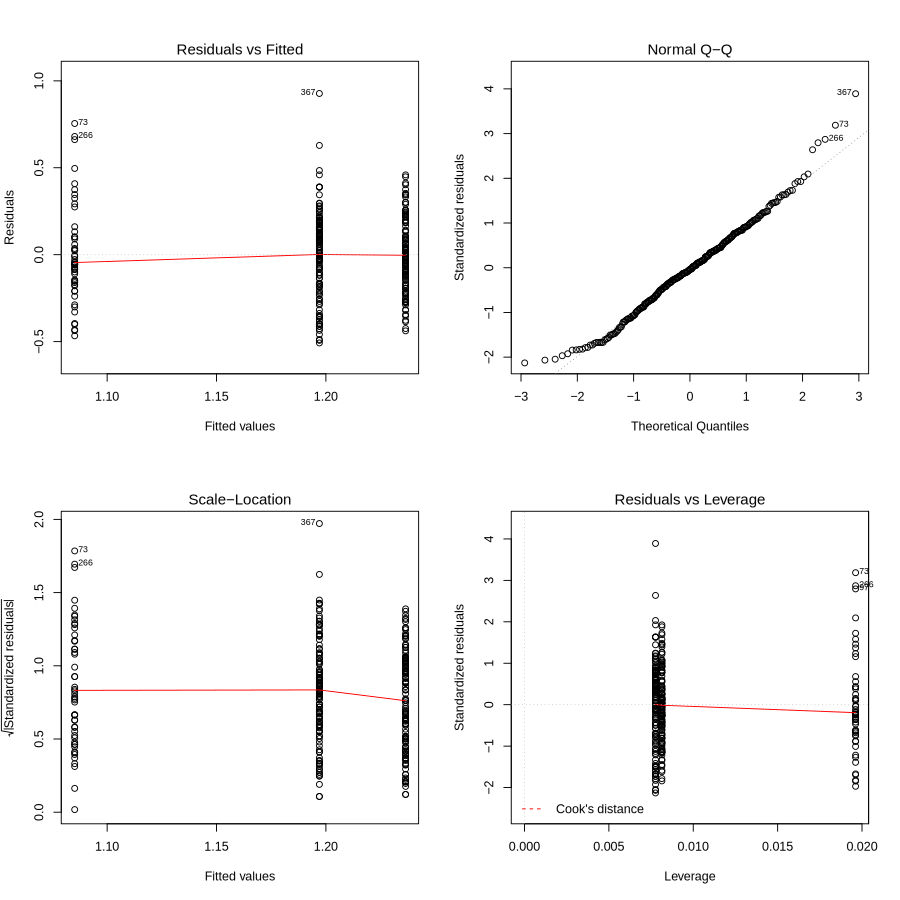
\includegraphics[width=0.8\textwidth]{modelDiag.pdf}	
\end{center}

Note that in regression, the predicted (or fitted) values from the 
model take a range along the relationship $y=a + bx$ (as we saw in the 
Figures \ref{fig:DiagModDragon} \& \ref{fig:DiagModDamsel}). For ANOVA, 
there are only a few predicted values --- one for each group mean. This 
means that the plots above look different but we are looking for the 
same things: is there constant variance at each fitted value and are 
the residuals normally distributed? The answer for this model looks to 
be yes.

\begin{compactitem}[$\quad\star$]
	\item Check the ground dwelling model in the same way.
\end{compactitem}
 
\section{Testing pairwise differences between levels}

The one thing that the trophic level model does not tell us is whether 
there is a difference in genome size between omnivores and herbivores 
--- both are compared to carnivores, but not to each other. This is 
because of the multiple pairwise testing problem mentioned in Chapter 
\ref{ch:t_F_tests} --- if you do 
lots of tests then you may find small $p$ values by chance and say 
something important is going on when it is just random chance. This is 
called a false positive or Type I error.
 
With a 95\% confidence interval, there is a 5\% chance of a false 
positive {\it per test} but there are ways of getting a 5\% chance 
across a set (or family) of tests. For  linear models, we can use 
Tukey's Honest Significant Difference test. We have to convert the {\tt 
lm} object into an {\tt aov} object first.

\begin{lstlisting}

> TukeyTroph <- TukeyHSD(aov(trophicLM))
> print(TukeyTroph)
	
   Tukey multiple comparisons of means
     95% family-wise confidence level
 
 Fit: aov(formula = trophicLM)
 
 $TrophicLevel
                        diff      lwr    upr  p adj
 Herbivore-Carnivore 0.11186  0.01863 0.2051 0.0139
 Omnivore-Carnivore  0.15128  0.05741 0.2452 0.0005
 Omnivore-Herbivore  0.03942 -0.03161 0.1104 0.3923
 
\end{lstlisting}

The table shows the following:
\begin{compactitem}

	\item The differences between the three possible pairs and then the 
	lower and upper bounds of the 95\% confidence interval for the 
	difference and a $p$ value. 

	\item In each case, we want to know if the difference could be zero: 
	does the 95\% confidence interval for each pair include zero.

	\item For the first two pairs,  carnivores versus omnivores and 
	herbivores, the confidence intervals do not include zero, so they are 
	significantly different. For the comparison between herbivores and 
	omnivores, the interval does include zero (difference = 0.039, 95\% 
	CI's limits are -0.032 \& 0.110), so these groups are not 
	significantly different.

	\item The $p$ values for the top two pairs are both larger (less 
	significant) than in the summary table. The test has made it harder 
	to find significant results.

\end{compactitem}

You can visualise these confidence intervals by plotting the Tukey 
test. You have to tweak the graphics parameters to get a clean plot 
though.

\begin{lstlisting}
> par(las=1, mar=c(4,10,3,1))
# las= 1 turns labels horizontal
# mar makes the left margin wider (bottom, left, top, right)
> plot(TukeyTroph)
\end{lstlisting} 

The result should be:

{\centering \includegraphics[width=0.8\textwidth]{TukeyPLot.pdf} }

\begin{compactitem}[$\quad\star$]
	\item Run the Tukey test in your script for both the trophic level 
	and ground dwelling models.
\end{compactitem}

\section{Are the factors independent?}

We've looked at two models, using trophic level and ground dwelling. It 
is worth asking whether these are independent factors. What if, for 
example, our herbivores are all big, ground dwellers? This is important 
to know because otherwise, a two-way ANOVA would not be appropriate. We 
will look at interactions in Chapter \ref{ch:MulExplInter}.

OK, so we want to know whether the two factors are independent. This is 
a job for the $\chi^2$ test!

\subsection{The Chi-square test and count data}

The Chi-square test, also known as $\chi^{2}$ test or chi-square test, 
is designed for scenarios where you want to statistically test how 
likely it is that an observed distribution of values is due to chance. 
It is also called a ``goodness of fit'' statistic, because it measures 
how well the observed distribution of data fits with the distribution 
that is expected if the variables of which measurements are made are 
independent. In our mammals example below, the two variables are 
trophic level and ground dwelling.

Note that a $\chi^{2}$ test is designed to analyze categorical data. 
That is the data have been counted (count data) and divided into 
categories. It is not meant for continuous data (such as body weight, 
genome size, or height). For example, if you want to test whether 
attending class influences how students perform on an exam, using test 
scores (from 0-100) as data would not be appropriate for a Chi-square 
test. However, arranging students into the categories ``Pass'' and 
``Fail'' and counting up how many fall in each categories would be 
appropriate. Additionally, the data in a Chi-square table (see below) 
should not be in the form of percentages -- only count data are 
allowed! 

\subsubsection{The Chi-square test with the mammals data}

We can easily build a table for a Chi-square test on the mammals 
data as follows:
  
\begin{lstlisting}
> factorTable <- table(mammals$GroundDwelling, mammals$TrophicLevel)
> print(factorTable) 

       Carnivore Herbivore Omnivore
   No         26        45       64
   Yes        22        62       40
\end{lstlisting}

Now let's run the test:

\begin{lstlisting}
> chisq.test(factorTable)
  
 	Pearson's Chi-squared test
 
 data:  factorTable 
 X-squared = 8.12, df = 2, p-value = 0.01725
\end{lstlisting}

The ``{\tt X-squared}'' value is the $\chi^{2}$ {\it test statistic}, akin to the 
t-value of the t-test or W value in the Wilcox test. 

The $\chi^{2}$ statistic is calculated as the sum of the quantity 
$$ \frac{(\mathrm{Observed} - \mathrm{Expected})^2}{\mathrm{Expected}} $$
across all the cells/categories in the table (so the sum would be over 
6 categories in our current mammals example).
   
``Observed'' is the observed proportion of data that fall in a 
certain category. For example, there are 26 species observed in the 
{\tt Carnivore}, {\tt No} category, and 22 in the {\tt Carnivore}, {\tt 
Yes} category. 

``Expected'' is what count would be expected if the values in each 
category we truly independent. Each cell has its own expected value, 
which is simply calculated as the count one would expect in each 
category if the value were generated in proportion to the total number 
seen in that category. So in our example, the expected value for the 
{\tt Carnivore}, {\tt No} category would be
$$26+22 \mathrm{~(Total~number~of~carnivore~species)} 
\times \frac{26+45+64 \mathrm{~(Total~number~in~the~''No''~category)}}{ 
26+22+45+62+64+40 \mathrm{~(Total~number~of~species)}}$$  
$$= 48 \times \frac{135}{259} = 25.02$$

The sum of all six (one for each cell in the table above) such 
calculations would be the $\chi^{2}$ value that R gave you through the 
{\tt chisq.test()} above --- try it!

Now back to the R output from the {\tt chisq.test()} above. Why df = 2? 
This is calculated as $DF = (r - 1) * (c - 1)$ where $r$ and $c$ are 
the number of rows and columns in the $\chi^{2}$ table, respectively. 
The same principle you learned before applies here; you lose one degree 
of freedom for each new level of information you need to estimate: 
there is uncertainity about the information (number of categories) in 
both rows and columns, so you need to lose one degree of freedom for 
each. 

Finally, note that the p-value is significant --- we can conclude that the 
factors aren't independent. From the table, carnivores can be either 
ground dwelling or not, but herbivores tend to be ground dwelling and 
omnivores tend not to be. Ah well... it's OK. We will look at a better 
way to analyze these data using ``interactions'' in Chapter 
\ref{ch:MulExplInter}.

\begin{compactitem}[$\quad\star$]
	\item Include and run the $\chi^2$ test in your script.
\end{compactitem}

\section{Saving data}

The last thing to do is to save a copy of the mammal data, including 
our new column of log data, for use in later chapters. 

\begin{compactitem}[$\quad\star$]
	\item Use this code in your script to create the saved data in you 
	{\tt Data} directory :
\end{compactitem}

\begin{lstlisting}
save(mammals, file='../Data/mammals.Rdata')
\end{lstlisting}	
 % anova}
\chapter{Linear Models: Multiple explanatory variables}
\label{ch:MulExpl}

Aims of this chapter\footnote{Here you work with the script file {\tt MulExpl.R}}:

\begin{compactitem}
	\item Including several explanatory variables in a model
	\item Interpreting summary tables for more complex models
\end{compactitem}

\section{Loading the data}

\begin{compactitem}[$\quad\star$]
	\item Create a new blank script called {\tt MulExpl.R} in your 
	{\tt Code} directory and add some introductory comments.

	\item Use {\tt load('../Data/mammals.Rdata')} to load the data saved 
	at the end of Chapter~\ref{ch:ANOVA}. Look back at the end of Chapter 
	\ref{ch:ANOVA} to see how you saved the RData file. If {\tt 
	mammals.Rdata} is missing, just import the data again using {\tt 
	read.csv("../Data/MammalData.csv")} and add the log C Value column to 
	the imported data frame again (got back to Chapter~\ref{ch:ANOVA} and 
	have a look if you have forgotten how).

	\item Use {\tt ls} and {\tt str} to check that the data has loaded 
	correctly.
	
\end{compactitem}

The models we looked at in Chapter~\ref{ch:ANOVA} explored whether 
the log genome size (C value, in picograms) of terrestrial mammals 
varied with trophic level and  whether or not the species is ground 
dwelling. We will now look at a single model that includes both 
explanatory variables. 

The first thing to do is look at the data again. In Chapter 
\ref{ch:regress}, we asked if carnivores or herbivores had larger 
genomes. Now we want to ask questions like: do ground-dwelling 
carnivores have larger genomes than arboreal or flying omnivores? We 
need to look at plots within groups. 

Before we do that, there is a lot of missing data in the data frame and 
we should make sure that we are using the same data for our plots and 
models. We will subset the data down to the complete data for the three 
variables:

\begin{lstlisting}
> mammals <- subset(mammals, select = c(GroundDwelling, TrophicLevel, 
logCvalue))
> mammals <- na.omit(mammals)
> str(mammals)

'data.frame':	259 obs. of  3 variables:
 $GroundDwelling: Factor w/ 2 levels "No","Yes": 2 2 2 2 2 1 2 1 1 1 ...
 $TrophicLevel  : Factor w/ 3 levels "Carnivore","Herbivore",..: 1 2 2 2 3 3 3 2 2 3 ...
 $logCvalue     : num  0.94 1.322 1.381 1.545 0.888 ...
  - attr(*, "na.action")=Class 'omit'  Named int [1:120] 2 4 7 9 10 11 14 15 20 21 ...
   .. ..- attr(*, "names")= chr [1:120] "2" "4" "7" "9" ...
\end{lstlisting}

\section{Boxplots within groups}

In Chapter~\ref{ch:regress}, we used the {\tt subset} option to fit a model just to 
dragonflies. You can use {\tt subset} with plots too.

\begin{compactitem}[$\quad\star$]
	\item Add {\tt par(mfrow=c(1,2))} to your script to split the 
	graphics into two panels.
	\item Copy the code from Chapter~\ref{ch:ANOVA} to create a boxplot 
	of genome size by trophic level into your script.
	\item Using this, and adding a {\tt subset} option to the code, 
	generate the plots shown in the figure below.
	\item You can use the option {\tt main} to add titles to a plot.
\end{compactitem}

\begin{center}
	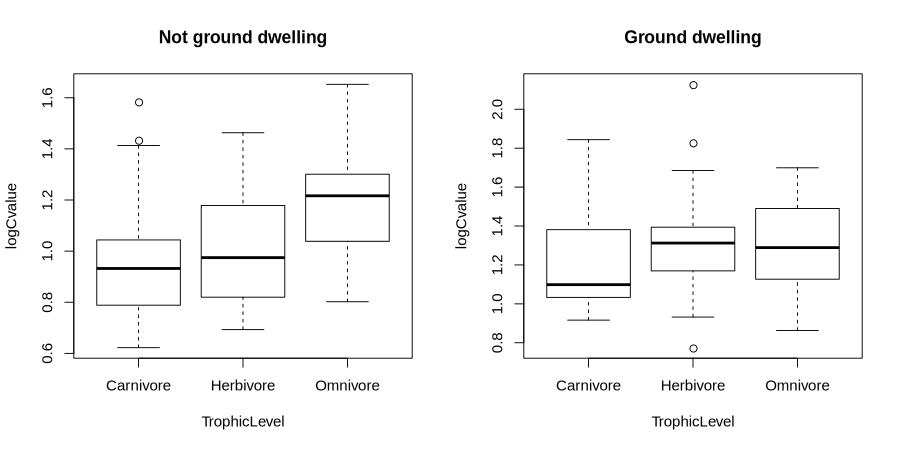
\includegraphics[width=1.0\textwidth]{boxplots.pdf}
\end{center} 

\section{{\tt lattice} again}

Recall that the {\tt lattice} package provides some very neat extra 
ways to plot data in groups. They look pretty but the downside is that 
they don't use the same graphics system --- all those {\tt par} 
commands are useless for these graphs. The defaults look good though!

\begin{lstlisting}
> library(lattice)
> bwplot(logCvalue ~ TrophicLevel | GroundDwelling, data= mammals)
\end{lstlisting}

\begin{center}
	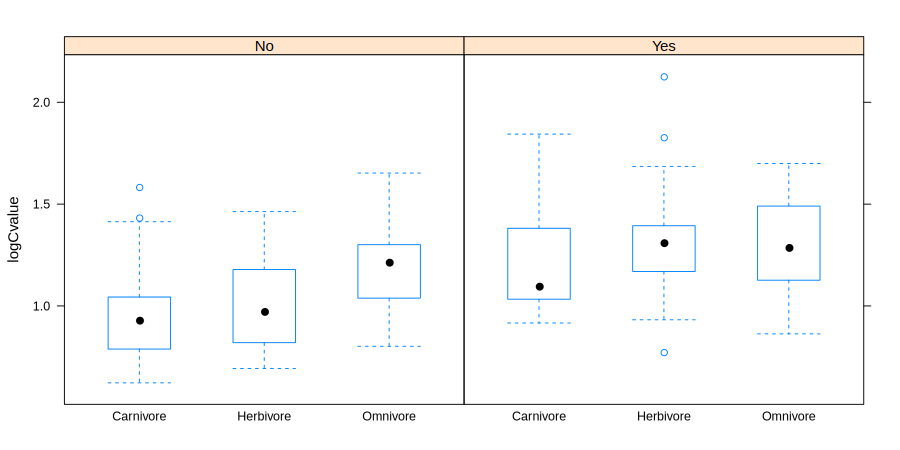
\includegraphics[width=1.0\textwidth]{bwplots.pdf}
\end{center}
	
The code {\tt logCvalue \textasciitilde{} TrophicLevel | 
GroundDwelling} means plot the relationship between genome size and 
trophic level, but group within levels of ground dwelling. We are using 
the function {\tt bwplot}, which is provided by {\tt lattice} to create 
box and whisker plots. 

\begin{compactitem}[$\quad\star$]
	\item Create the lattice plots above from within your script.
	\item Rearrange this code to have three plots, showing the box and 
	whisker plots for {\tt GroundDwelling}, grouped within the levels of 
	{\tt TrophicLevel}.
	\item Try reshaping the R plot window and running the command again. 
	Lattice tries to make good use of the available space when creating 
	lattice plots.
\end{compactitem}

\section{Barplots again}

We're going to make the barplot code from Chapter~\ref{ch:regress} even more 
complicated! This time we want to know the mean log genome size within 
combinations of {\tt TrophicLevel} and {\tt GroundDwelling}. We can 
still use {\tt tapply}, providing more than one grouping factor. We 
create a set of grouping factors like this:


\begin{lstlisting}
> groups <- list(mammals$GroundDwelling, mammals$TrophicLevel)
> groupMeans <- tapply(mammals$logCvalue, groups, FUN = mean)
> print(groupMeans)

     Carnivore Herbivore Omnivore
 No     0.9589     1.012    1.192
 Yes    1.2138     1.298    1.299
\end{lstlisting}

\begin{compactitem}[$\quad\star$]
	\item Copy this code into your script and run it.
	\item Use this code and the script from Chapter~\ref{ch:ANOVA} to get the set of 
	standard errors for the groups({\tt groupSE}). You should get this: 
\end{compactitem}

\begin{lstlisting}
     Carnivore Herbivore Omnivore
 No    0.04842   0.03419  0.02410
 Yes   0.05976   0.02787  0.03587
\end{lstlisting}

Now we can use {\tt barplot}. The default option for a barplot of a 
table is to create a stacked barplot, which is not what we want. The 
option {\tt beside=TRUE} makes the bars for each column appear side by 
side. Once again, we save the midpoints of the bars to add the error 
bars. The other options in the code below change the colours of the 
bars and the length of error bar caps.
% 
\begin{lstlisting}
	# get upper and lower standard error height
> upperSE <- groupMeans + groupSE
> lowerSE <- groupMeans - groupSE

# create barplot
> barMids <- barplot(groupMeans, ylim=c(0, max(upperSE)), beside=TRUE, 
ylab= ' log C value (pg) ' , col=c( ' white ' , ' grey70 '))

> arrows(barMids, upperSE, barMids, lowerSE, ang=90, code=3, len=0.05)
\end{lstlisting}

\begin{center}
	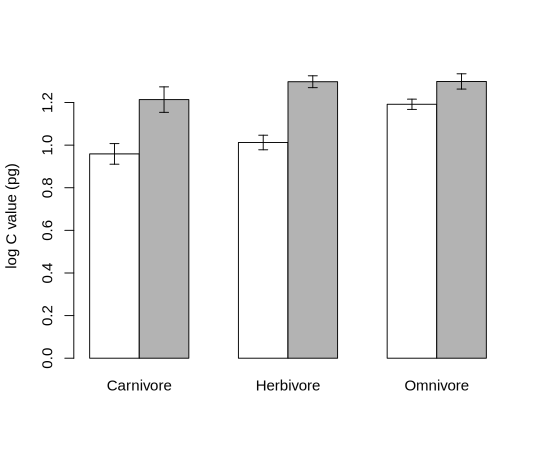
\includegraphics[width=0.6\textwidth]{barplot_1.pdf}
\end{center} 

\begin{compactitem}[$\quad\star$]
	\item Generate the barplot above and then edit your script to change 
	the colours and error bar lengths to your taste.
\end{compactitem}

\section{Plotting means and confidence intervals}

We'll use the {\tt plotmeans} function again as an exercise to change 
graph settings and to prepare figures for write ups. 

\begin{figure} \centering 
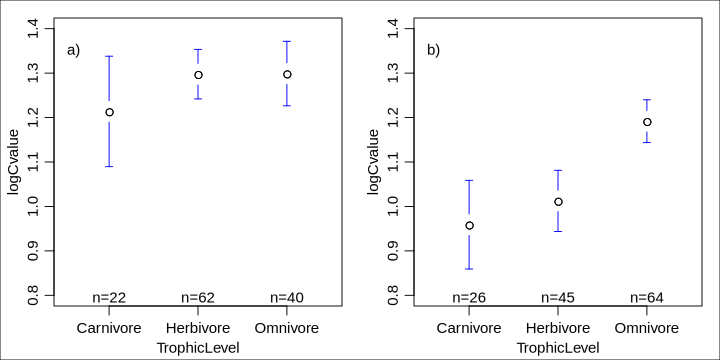
\includegraphics[width=0.9\textwidth]{plotmeans.pdf}

\caption{Means and 95\% confidence intervals for log genome size 
(picograms) in mammals for different trophic levels for a) ground 
dwelling species and b) other species.}

\label{fig:plotmeans}

\end{figure}

\begin{compactdesc}

\item [White space] The default options in R use wide margins and 
spaced out axes and take up a lot of space that could be used for 
plotting data. You've already seen the {\tt par} function and the 
options {\tt mfrow} for multiple plots and {\tt mar} to adjust margin 
size. The option {\tt mgp} adjusts the placement of the axis label, 
tick labels and tick locations. See {\tt ?par} for help on the these 
options.

\item [Main titles] Adding large titles to graphs is also a bad idea 
--- it uses lots of space to explain something that should be in the 
figure legend. With multiple plots in a figure, you have to label 
graphs so that the figure legend can refer to them. You can add labels 
using {\tt text(x,y,'label')}.

\item [Figure legends] A figure legend should give a clear stand-alone 
description of the whole figure. 

\item [Referring to figures] You {\it must} link from your text to 
your figures --- a reader has to know which figures refer to which 
results. So: `There are clear differences in mean genome size between 
species at different trophic levels and between ground dwelling and 
other species (Figure \ref{fig:plotmeans})'. 

\end{compactdesc}

\begin{compactitem}[$\quad\star$]
	
	\item Use {\tt plotmeans} from Chapter~\ref{ch:ANOVA} and the {\tt 
	subset} option to generate the two plots below. You will need to set 
	the {\tt ylim} option for the two plots to make them use the same $y$ 
	axis.
	
	\item Use {\tt text} to add labels --- the command {\tt par('usr')} 
	will show you the limits of the plot ($x_{min}, x_{max}, y_{min}, 
	y_{max}$) and help pick a location for the labels.

	\item Change the {\tt par} settings in your code and redraw the plots 
	to try and make better use of the space. In the example below, the 
	box shows the edges of the R graphics window.

\end{compactitem}
 
\section{Multiple explanatory variables}

All those graphs suggest:
\begin{compactitem}
 \item Carnivores have smaller genome size; omnivores have larger genome size. 
 \item Herbivores are somewhere in between, but not consistently.
 \item All ground dwelling mammals typically have larger genome sizes.
\end{compactitem}

We suspected these things from Chapter \ref{ch:ANOVA}, but now we can see 
that they might have separate effects. We'll fit a linear model to 
explore this and add the two explanatory variables together.
  
\begin{compactitem}[$\quad\star$]
\item This is an important section --- read it through carefully and 
ask questions if you are unsure. Copy the code into your script and add 
comments. {\it Do not just jump to the next action item}!
\end{compactitem}

\begin{lstlisting}
> model <- lm(logCvalue ~ TrophicLevel + GroundDwelling, data = mammals)	
\end{lstlisting}

We're going to do things right this time and check the model 
diagnostics before we rush into interpretation.

\begin{lstlisting}
> par(mfrow=c(2,2))
> plot(model)
\end{lstlisting}

\begin{center}
	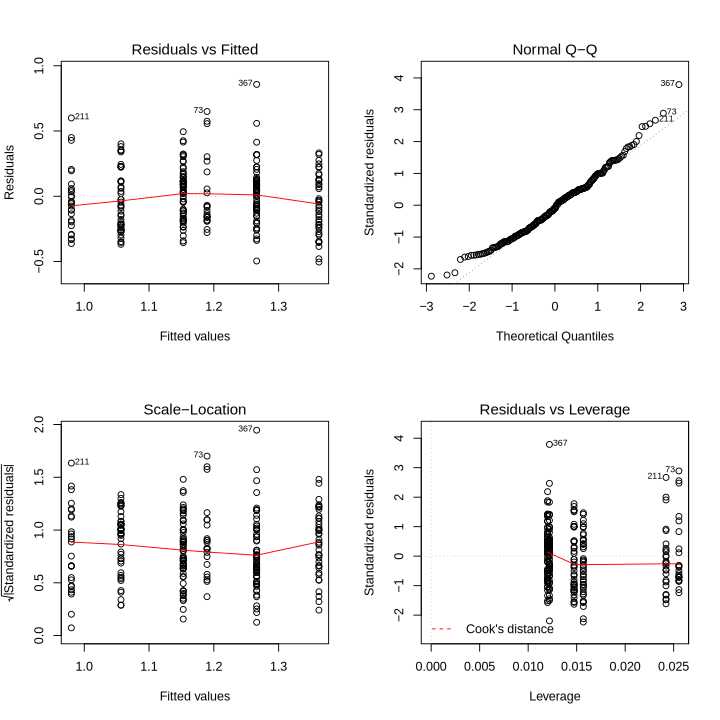
\includegraphics[width=\textwidth]{diagnostics1.pdf}
\end{center} 

There are six predicted values now - three trophic levels for each of 
the two levels of ground dwelling. Those plots look ok so now we can 
look  at the analysis of variance table:

\begin{lstlisting}
> anova(model)

 Analysis of Variance Table
 
 Response: logCvalue
                 Df Sum Sq Mean Sq F value  Pr(>F)    
 TrophicLevel     2   0.81   0.407    7.86 0.00049 ***
 GroundDwelling   1   2.75   2.747   53.04 4.1e-12 ***
 Residuals      255  13.21   0.052                    
 ---
 Signif. codes:  0 '***' 0.001 '**' 0.01 '*' 0.05 '.' 0.1 ' ' 1 
\end{lstlisting}

{\it Ignore the $p$ values}! Yes, they're highly significant but we 
want to understand the model, not rubber stamp it with `significant'.

\begin{compactitem}

 \item The sums of squares for the variables are both small compared to 
 the residual sums of squares --- there is lots of unexplained 
 variation. We can calculate the $r^2$ as explained sums of squares 
 over total sums of squares:
\[\frac{0.81 + 2.75}{0.81 + 2.75 + 13.21} = \frac{3.56}{16.77} = 0.212\]
 
\item Trophic level explain much less variation than ground dwelling 
--- this makes intuitive sense from the plots since there are big 
differences between Figure \ref{fig:plotmeans}a and 
\ref{fig:plotmeans}b, but small differences within.

\item We could also calculate a significance for the whole model by 
merging the terms. The total explained sums of squares of $0.81 + 2.75 
=3.56$ uses $2+1 =3$ degrees of freedom, so the mean sums of squares 
for all the terms together is $3.56/3=1.187$. Dividing this by the 
residual mean square of 0.052 gives an F of $1.187 / 0.052 = 22.83$.

\end{compactitem}

Now we can look at the summary table to see the coefficients. 

\begin{lstlisting}
> summary(model) 

 Call:
 lm(formula = logCvalue ~ TrophicLevel + GroundDwelling, data = mammals)
 
 Residuals:
     Min      1Q  Median      3Q     Max 
 -0.4990 -0.1784 -0.0146  0.1250  0.8624 
 
 Coefficients:
                       Estimate Std. Error t value Pr(>|t|)    
 (Intercept)             0.9798     0.0354   27.68  < 2e-16 ***
 TrophicLevelHerbivore   0.0766     0.0397    1.93    0.055 .  
 TrophicLevelOmnivore    0.1727     0.0398    4.34  2.0e-05 ***
 GroundDwellingYes       0.2095     0.0288    7.28  4.1e-12 ***
 ---
 Signif. codes:  0 '***' 0.001 '**' 0.01 '*' 0.05 '.' 0.1 ' ' 1 
 
 Residual standard error: 0.228 on 255 degrees of freedom
 Multiple R-squared: 0.212,	Adjusted R-squared: 0.203 
 F-statistic: 22.9 on 3 and 255 DF,  p-value: 3.6e-13 
 
\end{lstlisting}

Starting at the bottom, {\tt summary} has again calculated $r^2$ for us 
and also an $F$ statistic for the whole model, which matches the 
calculation above. 

The other important bits are the four coefficients. The intercept is 
now the reference level for two variables: it is the mean for 
carnivores that are not ground dwelling. We then have differences from 
this value for being an omnivore or herbivore and for being ground 
dwelling. There is a big change in genome size associated with ground 
dwelling and omnivory and both of these have large effects sizes, each 
introducing about a 20\% difference in genome size from the non-ground 
dwelling carnivores. In contrast, herbivory makes a small difference 
--- about 8\%. Because the difference is small and the standard error 
is large, the $t$ value suggests that this difference might arise just 
be chance. Put another way, it isn't significant.

The table below shows how these four coefficients combine to give the 
predicted values for each of the group means.

\[\begin{array}{|r|rrr|}
\hline
	       & \textrm{Carnivore} & \textrm{Herbivore} & \textrm{Omnivore}\\
\hline
\textrm{Not ground} & {\it 0.98} = 0.98    & {\it 0.98  + 0.08} =1.06    & {\it 0.98 + 0.17} =1.15 \\
\textrm{Ground}     & {\it 0.98 + 0.21} = 1.19    & {\it 0.98  + 0.08   + 0.21} =1.27   & {\it 0.98 + 0.17  + 0.21} =1.36\\
\hline
\end{array}\]

\section{Predicted values}

Getting the model predictions by hand in this way is tedious and error 
prone. There is handy function called {\tt predict} which uses the 
model directly to calculate values. The default is to give you the 
prediction for each point in the original data, but you can also ask 
for specific predictions.

The first thing to do is to set up a small data frame containing the 
explanatory values we want to use. The variable names and the level 
name have to match {\it exactly}, so we'll use the {\tt levels} 
function to get the names. We want to look at all six combinations, so 
we'll use the {\tt rep} function to set this up. The {\tt each=2} 
option repeats each value twice in succession; the {\tt times=3} 
options repeats the whole set of values three times.

\begin{lstlisting}
# data frame of combinations of variables
> gd <- rep(levels(mammals$GroundDwelling), times = 3)
> print(gd)

 [1] "No"  "Yes" "No"  "Yes" "No"  "Yes"
 
> tl <- rep(levels(mammals$TrophicLevel), each = 2)
> print(tl)

  [1] "Carnivore" "Carnivore" "Herbivore" "Herbivore" "Omnivore"  "Omnivore" 

> predVals <- data.frame(GroundDwelling = gd, TrophicLevel = tl)

\end{lstlisting}

Now we have the data frame of values we want, we can use predict. As 
when we created log values, we can save the output back into a new 
column in the data frame.

\begin{lstlisting}
> predVals$predict <- predict(model, newdata = predVals)
> print(predVals)

   GroundDwelling TrophicLevel predict
 1             No    Carnivore  0.9798
 2            Yes    Carnivore  1.1892
 3             No    Herbivore  1.0563
 4            Yes    Herbivore  1.2658
 5             No     Omnivore  1.1524
 6            Yes     Omnivore  1.3619
\end{lstlisting}

\begin{compactitem}[$\quad\star$]
	\item These are in the same order as the bars from your barplot. Make 
	a copy of the barplot and arrows code and then add the code below to 
	generate the plot. 
\end{compactitem}

\begin{lstlisting}
> points(barMids, predVals$predict, col= ' red ' , pch=5)
\end{lstlisting}

\begin{center}
	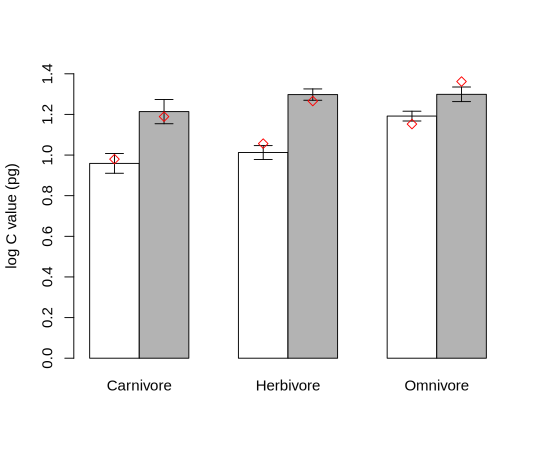
\includegraphics[width=0.6\textwidth]{barplotpred.pdf}
\end{center}

The red points do not match to the calculated means. This is because 
the model only includes a single difference between ground and 
non-ground species, which has to be the same for each trophic group. 
That is, there is no interaction between trophic level and ground / 
non-ground identity of each species in the current model.

The Chapter \ref{ch:MulExplInter} will look at interactions, which 
allows these values to differ using an interaction term in the model.
 % MulExpl}
\chapter{Linear Models: Multiple variables and interactions}
\label{ch:MulExplInter}

Aims of this chapter\footnote{Here you work with the script file {\tt MulExplInter.R}}:
\begin{compactitem}
	\item Creating more complex models, including ANCOVA
	\item Looking at interactions between variables
	\item Plotting predictions from models
\end{compactitem}

We will look at two models in this chapter:
\begin{compactenum}
	\item Model 1: Is mammalian genome size predicted by interactions 
	between trophic level and whether species are ground dwelling?
	\item ANCOVA: Is body size in Odonata predicted by interactions 
	between genome size and taxonomic suborder?
\end{compactenum}

So far, we have only looked at the independent effects of variables. 
For example, in the trophic level and ground dwelling model from 
Chapter \ref{ch:MulExpl}, we only looked for specific differences for being a omnivore 
{\it or} being ground dwelling, not for being specifically a {\it 
ground dwelling omnivore}. These independent effects of a variable are 
known as {\it main effects} and the effects of combinations of 
variables acting together are known as {\it interactions} --- they 
describe how the variables {\it interact}.

\section{Formulae with interactions in R}

We've already seen a number of different model formulae in R. They all 
use this syntax:\\
 {\tt  response variable \textasciitilde\ explanatory variable(s)} \\
but we are now going to add two extra pieces of syntax:

\begin{compactdesc}
	\item [{\tt y \textasciitilde\  a + b + a:b}] The {\tt a:b} means the 
	interaction between {\tt a} and {\tt b} --- do combinations of these 
	variables lead to different outcomes?
	\item [{\tt y \textasciitilde\  a * b}] This a shorthand for the model 
	above. The {\tt *} means fit {\tt a} and {\tt b} as main effects and 
	their interaction {\tt a:b}.
\end{compactdesc}	 

\section{Model 1: Mammalian genome size}

\begin{compactitem}[$\quad\star$]
	\item Make sure you have changed the working directory to {\tt Code} 
	in your stats coursework directory.
	\item Create a new blank script called `Interactions.R' and add some 
	introductory comments.
	\item Use {\tt load('mammals.Rdata')} to load the data.
\end{compactitem}

If {\tt mammals.Rdata} is missing, just import the data again using 
{\tt read.csv("../Data/MammalData.csv")}. You will then have to add the 
log C Value column to the imported data frame again. 

Let's refit the model from Chapter \ref{ch:MulExpl}, but including the 
interaction between trophic level and ground dwelling. We'll 
immediately check the model is appropriate:

\begin{lstlisting}
> model <- lm(logCvalue ~ TrophicLevel * GroundDwelling, data= mammals)
> par(mfrow=c(2,2), mar=c(3,3,1,1), mgp=c(2, 0.8,0))
> plot(model)	
\end{lstlisting}

This gives:
\begin{center}
	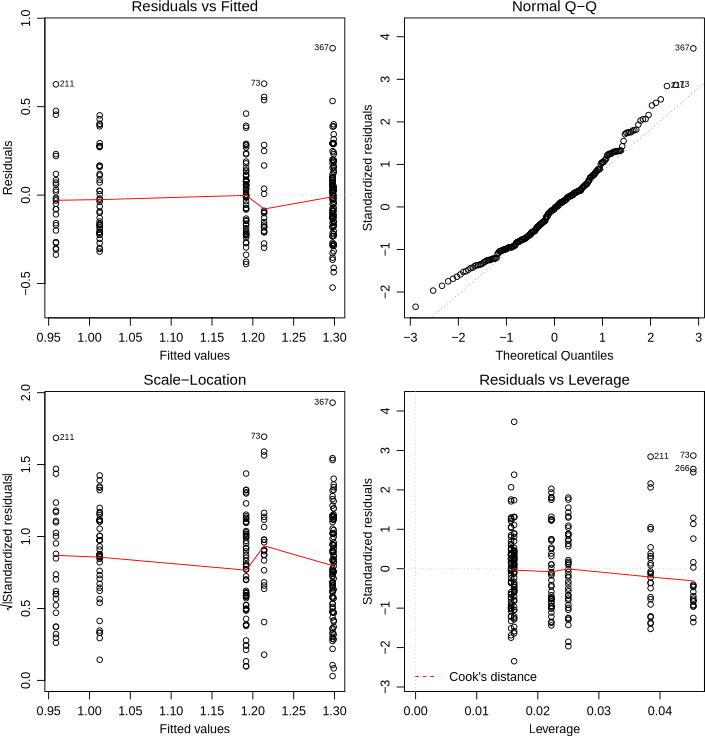
\includegraphics[width=\textwidth]{mamMod.pdf}
\end{center} 

Now, we'll examine the {\tt anova} and {\tt summary} outputs for the 
model:

\begin{lstlisting}
> anova(model)

 Analysis of Variance Table
 
 Response: logCvalue
                              Df Sum Sq Mean Sq F value  Pr(>F)    
 TrophicLevel                  2   0.81   0.407    8.06  0.0004 ***
 GroundDwelling                1   2.75   2.747   54.40 2.3e-12 ***
 TrophicLevel:GroundDwelling   2   0.43   0.216    4.27  0.0150 *  
 Residuals                   253  12.77   0.050                    
 ---
 Signif. codes:  0 '***' 0.001 '**' 0.01 '*' 0.05 '.' 0.1 ' ' 1 
\end{lstlisting}

Compared to the model from Chapter \ref{ch:MulExpl}, there is an extra line at the 
bottom. The top two are the same and show that trophic level and ground 
dwelling both have independent main effects. The extra line shows that 
there is also an interaction between the two. It doesn't explain a huge 
amount of variation, about half as much as trophic level, but it is 
significant.

Again, we can calculate the $r^2$ for the model: \[ \frac{0.81 + 2.75 + 
0.43}{0.81+2.75+0.43+12.77} = 0.238 \] The model from Chapter 
\ref{ch:MulExpl} without the interaction had an $r^2 = 0.212$ --- our 
new model explains 2.6\% more of the variation in the data.

The summary table is as follows:

 \begin{lstlisting}
>summary(model)
 
 Call:
 lm(formula = logCvalue ~ TrophicLevel * GroundDwelling, data = mammals)
 
 Residuals:
    Min     1Q Median     3Q    Max 
 -0.523 -0.171 -0.010  0.119  0.831 
 
 Coefficients:
                                         Estimate Std. Error t value Pr(>|t|)    
 (Intercept)                               0.9589     0.0441   21.76  < 2e-16 ***
 TrophicLevelHerbivore                     0.0535     0.0554    0.97  0.33460    
 TrophicLevelOmnivore                      0.2328     0.0523    4.45  1.3e-05 ***
 GroundDwellingYes                         0.2549     0.0651    3.92  0.00012 ***
 TrophicLevelHerbivore:GroundDwellingYes   0.0303     0.0786    0.39  0.69979    
 TrophicLevelOmnivore:GroundDwellingYes   -0.1476     0.0793   -1.86  0.06384 .  
 ---
 Signif. codes:  0 '***' 0.001 '**' 0.01 '*' 0.05 '.' 0.1 ' ' 1 
 
 Residual standard error: 0.225 on 253 degrees of freedom
   (120 observations deleted due to missingness)
 Multiple R-squared: 0.238,	Adjusted R-squared: 0.223 
 F-statistic: 15.8 on 5 and 253 DF,  p-value: 1.5e-13 
\end{lstlisting}

The lines in this are:
\begin{compactitem}
	\item The reference level (intercept) for non ground dwelling 
	carnivores. (The reference level is decided just by the alphabetic 
	order of the levels)
	\item Two differences for being in different trophic levels.
	\item One difference for being ground dwelling
	\item Two new differences that give specific differences for ground 
	dwelling herbivores and omnivores.
\end{compactitem}

The first four lines, as in the model from Chapter~\ref{ch:ANOVA}, 
which would allow us to find the predicted values for each group {\it if the size of the differences did not vary between levels because of the interactions}. That is, this part of the model only includes a single difference ground and non-ground species, which has to be the same for each trophic group because it  ignores interactions between trophic level and ground / non-ground
identity of each species. The last two lines then give the estimated coefficients associated with the interaction terms, and allow cause the size of differences to vary between levels because of the further effects of interactions.

The table below show how these combine to give the predictions for each 
group combination, with those two new lines show in red:

\[\begin{array}{|r|r|r|}
\hline
 & \textrm{Not ground} &  \textrm{Ground} \\
\hline
\textrm{Carnivore} & 0.96 = 0.96 &  0.96+0.25=1.21 \\
\textrm{Herbivore} & 0.96 + 0.05 = 1.01 & 0.96+0.05+0.25{\color{red}+0.03}=1.29\\
\textrm{Omnivore} & 0.96 + 0.23 = 1.19 & 0.96+0.23+0.25{\color{red}-0.15}=1.29\\
\hline
\end{array}\]

So why are there two new coefficients? For interactions between two 
factors, there are always $(n-1)\times(m-1)$ new coefficients, where 
$n$ and $m$ are the number of levels in the two factors (Ground dwelling or not: 2 levels and trophic level: 3 levels, in our current example). So in this model, $(3-1) \times (2-1) =2$. It is easier to understand why graphically: 
the prediction for the white boxes below can be found by adding the 
main effects together but for the grey boxes we need to find specific 
differences and so there are $(n-1)\times(m-1)$ interaction 
coefficients to add.

\[
n=4,m=4\quad
\begin{array}{|c|c|c|c|}
\hline
 & & & \\ 
\hline
 & \gc & \gc  &  \gc \\ 
\hline
 & \gc  & \gc  & \gc \\ 
\hline
 &  \gc &  \gc & \gc \\ 
\hline
\end{array}
\quad n=3,m=6 \quad
\begin{array}{|c|c|c|c|c|c|}
\hline
 & & & & &\\ 
\hline
 & \gc & \gc  &  \gc &  \gc &  \gc \\ 
\hline
 & \gc  & \gc  & \gc  &  \gc &  \gc\\ 
\hline
\end{array}
\]

If we put this together, what is the model telling us? 
\begin{compactitem}
\item Herbivores have the same genome sizes as carnivores, but 
omnivores have larger genomes.
\item Ground dwelling mammals have larger genomes.
\item These two findings suggest that ground dwelling omnivores should 
have extra big genomes. However, the interaction shows they are smaller 
than expected and are, in fact, similar to ground dwelling herbivores.
\end{compactitem}

Note that although the interaction term in the {\tt anova} output is 
significant, neither of the two coefficients in the {\tt summary} has a 
$p<0.05$. There are two weak differences (one very weak, one nearly 
significant) that together explain significant variance in the data.

\begin{compactitem}[$\quad\star$]
	\item Copy the code above into your script and run the model.
	\item Make sure you understand the output!
\end{compactitem}

Just to make sure the sums above are correct, we'll use the same code 
as in \ref{ch:MulExpl} to get R to calculate predictions for us: 

\begin{lstlisting}
# a data frame of combinations of variables
> gd <- rep(levels(mammals$GroundDwelling), times = 3)
> print(gd)
 [1] "No"  "Yes" "No"  "Yes" "No"  "Yes"

> tl <- rep(levels(mammals$TrophicLevel), each = 2)
> print(tl)

 [1] "Carnivore" "Carnivore" "Herbivore" "Herbivore" "Omnivore"  "Omnivore" 

# New data frame
> predVals <- data.frame(GroundDwelling = gd, TrophicLevel = tl)

# predict using the new data frame
> predVals$predict <- predict(model, newdata = predVals)
> print(predVals)
 
    GroundDwelling TrophicLevel predict
 1             No    Carnivore  0.9589
 2            Yes    Carnivore  1.2138
 3             No    Herbivore  1.0125
 4            Yes    Herbivore  1.2977
 5             No     Omnivore  1.1918
 6            Yes     Omnivore  1.2990
\end{lstlisting}

\begin{compactitem}[$\quad\star$]
	\item Run these predictions in your script.
\end{compactitem}

If we plot these data points onto the barplot from Chapter 
\label{ch:MulExpl}, they now lie exactly on the mean values, 
because we've allowed for interactions. The triangle on this plot shows 
the predictions for ground dwelling omnivores from the main effects 
($0.96 + 0.23  + 0.25 = 1.44$), the interaction of $-0.15$ pushes the 
prediction back down.

\begin{center}
	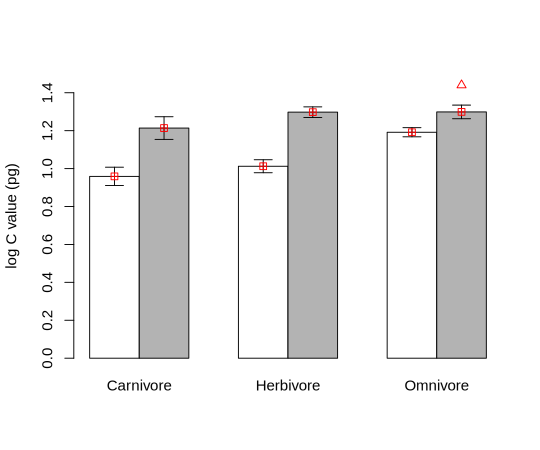
\includegraphics[width=0.8\textwidth]{predPlot.pdf} 
\end{center} 

\section{ANCOVA: Body Weight in Odonata}

We'll go all the way back to the regression analyses from 
Chapter~\ref{ch:regress}. Remember that we fitted two separate 
regression lines to the data for damselflies and dragonflies. We'll now 
use an interaction to fit these in a single model. This kind of linear 
model --- with a mixture of continuous variables and factors --- is 
often called an {\it analysis of covariance}, or ANCOVA. That is, 
ANCOVA is a type of linear model that blends ANOVA and regression. 
ANCOVA evaluates whether population means of a dependent variable are 
equal across levels of a categorical independent variable, while 
statistically controlling for the effects of other continuous variables 
that are not of primary interest, known as covariates. 

{\it That is, this is still a linear model, but with one categorical and one or more continuous predictors}.

\begin{compactitem}[$\quad\star$]
	\item Load the data: {\tt odonata <- read.csv('../Data/GenomeSize.csv')}.
	\item Create two new variables in the {\tt odonata} data set called 
	{\tt logGS} and {\tt logBW} containing log genome size and log body 
	weight.
\end{compactitem}

The models we fitted before looked like this:

\begin{center}
	\includegraphics[width=0.7\textwidth]{dragonData.pdf} 
\end{center} 

We can now fit the model of body weight as a function of both genome 
size and suborder:

\begin{lstlisting}
> odonModel <- lm(logBW ~ logGS * Suborder, data = odonata)
\end{lstlisting}

Again, we'll look at the {\tt anova} table first:

\begin{lstlisting}
> anova(odonModel)
 
 Analysis of Variance Table
 
 Response: logBW
                Df Sum Sq Mean Sq F value  Pr(>F)    
 logGS           1    1.1     1.1    2.71     0.1    
 Suborder        1  112.0   112.0  265.13 < 2e-16 ***
 logGS:Suborder  1    9.1     9.1   21.65 1.1e-05 ***
 Residuals      94   39.7     0.4                    
 ---
 Signif. codes:  0 '***' 0.001 '**' 0.01 '*' 0.05 '.' 0.1 ' ' 1 
\end{lstlisting}

Interpreting this gives the following:
\begin{compactitem}

	\item There is no significant main effect of log genome size. The 
	{\it main} effect is the important thing here --- genome size is 
	hugely important but does very different things for the two different 
	suborders. If we ignored {\tt Suborder}, there isn't an overall 
	relationship: the average of those two lines is pretty much flat.

	\item There is a very strong main effect of Suborder: the mean body 
	weight in the two groups are very different.

	\item There is a strong interaction between suborder and genome size. 
	This is an interaction between a factor and a continuous variable and 
	shows that the {\it slopes} are different for the different factor 
	levels.

\end{compactitem}
	
The summary table looks like this:
\begin{lstlisting}
> summary(odonModel)
 
 Call:
 lm(formula = logBW ~ logGS * Suborder, data = odonata)
 
 Residuals:
     Min      1Q  Median      3Q     Max 
 -1.3243 -0.3225  0.0073  0.3962  1.4976 
 
 Coefficients:
                         Estimate Std. Error t value Pr(>|t|)    
 (Intercept)              -2.3995     0.0848  -28.31  < 2e-16 ***
 logGS                     1.0052     0.2237    4.49  2.0e-05 ***
 SuborderZygoptera        -2.2489     0.1354  -16.61  < 2e-16 ***
 logGS:SuborderZygoptera  -2.1492     0.4619   -4.65  1.1e-05 ***
 ---
 Signif. codes:  0 '***' 0.001 '**' 0.01 '*' 0.05 '.' 0.1 ' ' 1 
 
 Residual standard error: 0.65 on 94 degrees of freedom
   (2 observations deleted due to missingness)
 Multiple R-squared: 0.755,	Adjusted R-squared: 0.747 
 F-statistic: 96.5 on 3 and 94 DF,  p-value: <2e-16 
 
\end{lstlisting}

The first thing to note is that the $r^2$ value is really high. The 
model explains three quarters (0.752) of the variation in the data. 
Next, there are four coefficients:

\begin{compactitem}
	\item The intercept is for the first level of {\tt Suborder}, which 
	is Anisoptera (dragonflies).
	\item The next line, for log genome size, is the slope for Anisoptera.
	\item We then have a coefficient for  the second level of {\tt 
	Suborder}, which is Zygoptera (damselflies). As with the first model, 
	this difference in factor levels is a difference in mean values and 
	shows the difference in the intercept for Zygoptera. 
	\item The last line is the interaction between {\tt Suborder} and 
	{\tt logGS}. This shows how the slope for Zygoptera differs from the 
	slope for Anisoptera.
\end{compactitem}

How do these hang together to give the two lines shown in the model? We 
can calculate these by hand:
\begin{align*}
	\textrm{Body Weight} &= -2.40 + 1.01 \times \textrm{logGS} & \textrm{[Anisoptera]}\\
	\textrm{Body Weight} &= (-2.40 -2.25) + (1.01 - 2.15) \times \textrm{logGS} & \textrm{[Zygoptera]}\\
	                     &= -4.65 - 1.14 \times \textrm{logGS} \\
\end{align*}


\begin{compactitem}[$\quad\star$]
	\item Add the code into your script and check that you understand the 
	outputs.
\end{compactitem}

We'll use the {\tt predict} function to get the predicted values from 
the model and add lines to the plot above.

First, we'll create a set of numbers spanning the range of genome size:

\begin{lstlisting}	
#get the range of the data
> rng <- range(odonata$logGS)
#get a sequence from the min to the max with 100 equally spaced values
> LogGSForFitting <- seq(rng[1], rng[2], length = 100)
\end{lstlisting}
Have a look at these numbers:
 
\begin{lstlisting}	
	print(LogGSForFitting)
\end{lstlisting}
 
We can now use the model to predict the values of body weight at each 
of those points for each of the two suborders.  We've added {\tt 
se.fit=TRUE} to the function to get the standard error around the 
regression lines. Note that we are now using 

\begin{lstlisting}
#get a data frame of new data for the order
> ZygoVals <- data.frame(logGS = LogGSForFitting, Suborder = "Zygoptera")

#get the predictions and standard error
> ZygoPred <- predict(odonModel, newdata = ZygoVals, se.fit = TRUE)

#repeat for anisoptera
AnisoVals <- data.frame(logGS = LogGSForFitting, Suborder = "Anisoptera")

AnisoPred <- predict(odonModel, newdata = AnisoVals, se.fit = TRUE)
\end{lstlisting}

Both {\tt AnisoPred} and {\tt ZygoPred} contain predicted values 
(called {\tt fit}) and standard error values (called {\tt se.fit}) for 
each of the values in our generated values in {\tt LogGSForFitting} for each of the two suborders.

We can add the predictions onto a plot like this:

\begin{lstlisting}
# plot the scatterplot of the data
> plot(logBW ~ logGS, data = odonata, col = Suborder)
# add the predicted lines
> lines(AnisoPred$fit ~ LogGSForFitting, col = "black")
> lines(AnisoPred$fit + AnisoPred$se.fit ~ LogGSForFitting, col = "black", lty = 2)
> lines(AnisoPred$fit - AnisoPred$se.fit ~ LogGSForFitting, col = "black", lty = 2)
\end{lstlisting}

\begin{compactitem}[$\quad\star$]
	\item Copy the prediction code into your script and run the plot 
	above. Copy and modify the last three lines to add the lines for the 
	Zygoptera. Your final plot should look like this.
\end{compactitem}

\begin{center}
	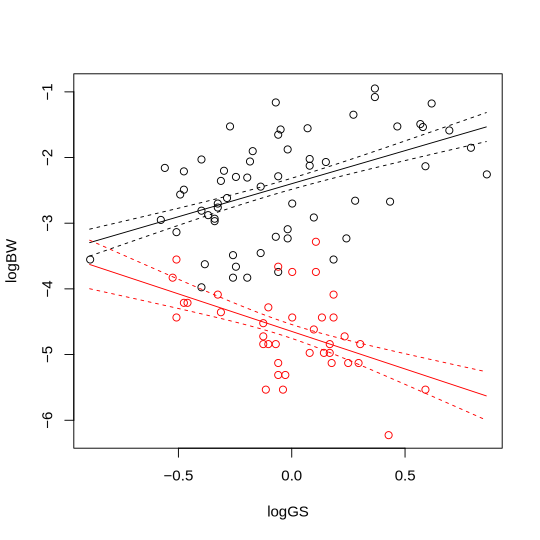
\includegraphics[width=0.7\textwidth]{odonPlot.pdf}
\end{center}  

 % MulExplInter}
\chapter{Linear Models: Model simplification}
\label{chap:ModelSimp}

Aims of this chapter\footnote{Here you work with the script file {\tt ModelSimp.R}}:
\begin{compactitem}
	\item Simplifying complex models by removing non-explanatory terms
\end{compactitem}

In biology, we often use statistics to compare competing hypotheses in 
order to work out the simplest explanation for some data. This often 
involves collecting several explanatory variables that describe 
different hypotheses and then fitting them together in a single model, 
and often including interactions between those variables.

In all likelihood, not all of these model {\it terms} will be 
important. If we remove unimportant terms, then the explanatory power 
of the model will get worse, but might not get significantly worse. 

\begin{quotation} \it
``It can scarcely be denied that the supreme goal of all theory is to 
make the irreducible basic elements as simple and as few as possible 
without having to surrender the adequate representation of a single 
datum of experience.'' 

\em Albert Einstein

\end{quotation}

\noindent Or to paraphrase:

\begin{quotation}\it
``Everything should be made as simple as possible, but no simpler.''
\end{quotation}

The approach we will look at is to start with a {\it maximal model} 
--- the model that contains everything that might be important --- and 
simplify it towards the {\it null model} --- the model that says that 
none of your variables are important. Hopefully, there is a point 
somewhere in between where you can't remove any further terms without 
making the model significantly worse: this is called the {\it minimum 
adequate model}.


\begin{tikzpicture}[every node/.style={draw=black!70, very thick, rectangle, rounded corners}]
\node[fill=black!10, minimum width=4 cm] (a) at (0,0) {Maximal model};
\node[fill=black!10, minimum width=4 cm] (b) at (5,0) {Minimum adequate model};
\node[fill=black!10, minimum width=4 cm] (c) at (10,0) {Null model};
\draw [draw=black!70, very thick, -stealth, shorten >= 1mm] (a.east) -- (b.west);
\draw [draw=black!70, very thick, -stealth, shorten >= 1mm] (b.east) -- (c.west);
\end{tikzpicture}

\section{A maximal model}

We'll be using the mammal dataset for this practical, so once again:

\begin{compactitem}[$\quad\star$]
	\item Make sure you have changed the working directory to your 
	stats module {\tt Code} folder.
	\item Create a new blank script called `MyModelSimp.R'.
	\item Load the mammals data into a data frame called {\tt mammals}.
\end{compactitem}

In Chapters 5 \& \ref{ch:MulExplInter}, we looked at how the 
categorical variables {\tt GroundDwelling} and {\tt TrophicLevel} 
predicted genome size in mammals. In this chapter, we will add in two 
more continuous variables: litter size and body mass. The first thing 
we will do is to log both variables and reduce the dataset to the rows 
for which all of these data are available:

\begin{lstlisting}
#get logs of continuous variables
> mammals$logLS <- log(mammals$LitterSize)
> mammals$logCvalue <- log(mammals$meanCvalue)
> mammals$logBM <- log(mammals$AdultBodyMass_g)

# reduce dataset to five key variables
> mammals <- subset(mammals, select = c(logCvalue, logLS, logBM, 
TrophicLevel, GroundDwelling))

# remove the row with missing data
> mammals <- na.omit(mammals)
\end{lstlisting}

\begin{compactitem}[$\quad\star$]
	\item Copy the code above into your script and run it
	\item Check that the data you end up with has this structure:
\end{compactitem}

\begin{lstlisting}
 'data.frame':	240 obs. of  5 variables:
 $logCvalue     : num  0.94 1.322 1.381 1.545 0.888 ...
 $logLS         : num  1.1 1.12 0 0 1.52 ...
 $logBM         : num  10.83 4.87 11.46 10.86 3.23 ...
 $TrophicLevel  : Factor w/ 3 levels "Carnivore","Herbivore",..: 1 2 2 2 3 3 3 2 2 3 ...
 $GroundDwelling: Factor w/ 2 levels "No","Yes": 2 2 2 2 2 1 2 1 1 1 ...
  - attr(*, "na.action")=Class 'omit'  Named int [1:139] 2 4 7 9 10 11 14 15 20 21 ...
   .. ..- attr(*, "names")= chr [1:139] "2" "4" "7" "9" ...
\end{lstlisting}

Now we'll fit a model including all of these variables and all of the 
interactions:

\begin{lstlisting}
> model <- lm(formula = logCvalue ~ logLS * logBM * TrophicLevel * 
GroundDwelling, data = mammals)
\end{lstlisting}

\begin{compactitem}[$\quad\star$]
	\item Run this model in your script.
	\item Look at the output of {\tt anova(model)} and {\tt 
	summary(model)}.
\end{compactitem}

Scared? Don't be! There are a number of points to this exercise:
\begin{enumerate}

	\item These tables show exactly the kind of output you've seen 
	before. Sure, there are lots of rows but each row is just asking 
	whether a model term ({\tt anova}) or a model coefficient ({\tt 
	summary}) is significant.

	\item Some of the rows are significant, others aren't: some of the 
	model terms are not explanatory.

	\item The two tables show slightly different things - lots of stars 
	for the {\tt anova} table and only a few for the {\tt summary} table.

	\item That last line in the {\tt anova} table: {\tt 
	logLS:logBM:TrophicLevel:GroundDwelling}. This is an interaction of 
	four variables capturing how the slope for litter size changes for 
	different body masses for species in different trophic groups and 
	which are arboreal or ground dwelling. Does this seem easy to 
	understand?
\end{enumerate}

The real lesson here is that it is easy to fit complicated models in R. 
{\it Understanding and explaining them is a different matter}. The 
temptation is always to start with the most complex possible model but 
this is rarely a good idea.

\section{A better maximal model}

Instead of all possible interactions, we'll consider two-way 
interactions: how do pairs of variables affect each other? There is a 
shortcut for this: {\tt y \textasciitilde{} (a + b + 
c)\textasciicircum{}2} gets all two way combinations of the variables 
in the brackets, so is a quicker way of getting this model:

{\tt y \textasciitilde{} a + b + c + a:b + a:c + b:c}.

So let's use this to fit a simpler maximal model:

\begin{lstlisting}
> model <- lm(logCvalue ~ (logLS + logBM + TrophicLevel + GroundDwelling)^2, data = mammals)
\end{lstlisting}

The {\tt anova} table for this model looks like this:

\begin{lstlisting}
> anova(model)

 Analysis of Variance Table
 
 Response: logCvalue
                              Df Sum Sq Mean Sq F value  Pr(>F)    
 logLS                         1   0.99   0.989   25.72 8.2e-07 ***
 logBM                         1   3.03   3.032   78.83 < 2e-16 ***
 TrophicLevel                  2   0.48   0.239    6.21  0.0024 ** 
 GroundDwelling                1   0.11   0.110    2.87  0.0915 .  
 logLS:logBM                   1   0.27   0.275    7.15  0.0081 ** 
 logLS:TrophicLevel            2   0.19   0.095    2.48  0.0862 .  
 logLS:GroundDwelling          1   0.14   0.136    3.55  0.0609 .  
 logBM:TrophicLevel            2   0.09   0.044    1.14  0.3230    
 logBM:GroundDwelling          1   0.88   0.883   22.96 3.0e-06 ***
 TrophicLevel:GroundDwelling   2   0.04   0.022    0.58  0.5607    
 Residuals                   225   8.65   0.038                    
 ---
 Signif. codes:  0 '***' 0.001 '**' 0.01 '*' 0.05 '.' 0.1 ' ' 1 
\end{lstlisting}

The first lines are the {\it main effects}, which are all significant 
or near significant. Then there are the six interactions. One of these 
is very significant: {\tt logBM:GroundDwelling}, which suggests that 
the slope of log C value with body mass differs between ground dwelling 
and non-ground dwelling species. The other interactions are 
non-significant although some are close. 

\begin{compactitem}[$\quad\star$]
	\item Run this model in your script.
	\item Look at the output of {\tt anova(model)} and {\tt 
	summary(model)}.
	\item Check the model diagnostic plots.
\end{compactitem}

\section{Model simplification}

Model simplification is not a simple process. Each time you remove a 
term from a model, the model will change: the model will get worse, 
since some of the sums of squares are no longer explained, but the 
remaining variables may take over.

The first question is: {\it what terms can you remove from a model}? 
Obviously, you only want to remove non-significant terms, but there is 
another rule -- you cannot remove a main effect or an interaction while 
those main effects or interactions are present in a more complex 
interaction. For example, in the model {\tt y \textasciitilde{} a + b + 
c + a:b + a:c + b:c}, you cannot drop {\tt c} without dropping both 
{\tt a:c} and {\tt b:c}. 

The R function {\tt drop.scope} tells you what you can drop from a 
model. Some examples:
\begin{lstlisting}
> drop.scope(model)
 [1] "logLS:logBM"                 "logLS:TrophicLevel"         
 [3] "logLS:GroundDwelling"        "logBM:TrophicLevel"         
 [5] "logBM:GroundDwelling"        "TrophicLevel:GroundDwelling"

> drop.scope(y ~ a + b + c + a:b)
 [1] "c"   "a:b"
> drop.scope(y ~ a + b + c + a:b + b:c + a:b:c)
 [1] "a:b:c"
\end{lstlisting}

Model simplification is an iterative process. The flow diagram below 
shows how it works: at each stage you try and find an acceptable 
simplification. If successful, then you start again with the new 
simpler model and try and find a way to simplify this, until 
eventually, you can't find anything more to remove.

\noindent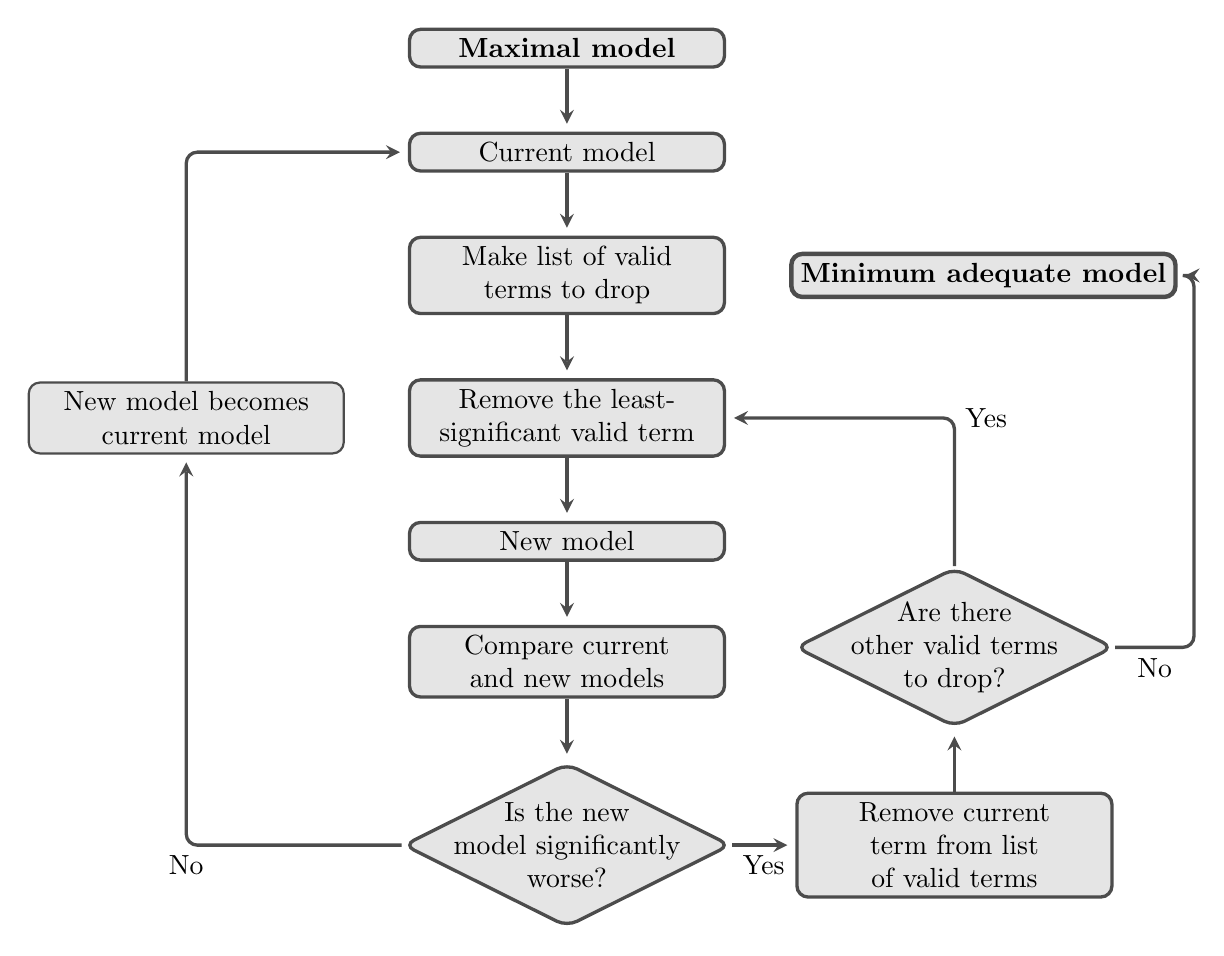
\begin{tikzpicture}
	[bx/.style={draw=black!70, very thick, rectangle, align=center,
	                    rounded corners, fill=black!10, minimum width=4 cm},
	 every path/.style={draw=black!70, very thick, -stealth, shorten >= 1mm},
	node distance=0.8cm]
	\node[bx] (a) at (0,0) {\bf Maximal model};
	\node[bx, below= of a] (b) {Current model};
	\node[bx, below= of b] (b2) {Make list of valid\\terms to drop};	
	\node[bx, below=of b2] (c) {Remove the least-\\significant valid term};
	\node[bx, below=of c] (d) {New model};
	\node[bx, below=of d] (e) {Compare current \\and new models};
	\node[bx, below=of e, diamond, aspect=2, inner sep=-1.5 mm] (f) {Is the new\\ model significantly\\ worse?};
	\node[bx, right=of f] (g) {Remove current\\ term from list \\of valid terms};
	\node[bx, above=of g, diamond, aspect=2, inner sep=-1.5 mm] (h) {Are there\\ other  valid terms \\to drop?};
	\node[bx, right=of b2, ultra thick] (i)  {\bf Minimum adequate model};
	\node[bx, left=of c, thick] (j)  {New model becomes\\ current model};

	\draw (a.south) -- (b.north);
	\draw (b.south) -- (b2.north);
	\draw (b2.south) -- (c.north);
	\draw (c.south) -- (d.north);
	\draw (d.south) -- (e.north);
	\draw (e.south) -- (f.north);
	\draw[rounded corners] (f.west) -| node[below]{No} (j.south) ;
	\draw[rounded corners] (j.north) |-  (b.west) ;
	\draw (f.east) -- node[below]{Yes} (g.west);
	\draw (g.north) --  (h.south);	
	\draw[rounded corners, label distance=1cm] (h.north)   |- node[right, pos=0.5]{Yes}(c.east);
	\draw[rounded corners] (h.east)  --  node[below]{No} ++(1,0) |- (i.east);
\end{tikzpicture}

As always, we can use an $F$ test to compare two models and see if they 
have significantly different explanatory power. Here, significance is a 
bad thing --- it means that we've removed a term that makes the model 
significantly worse.

The last thing we need to do is work out how to remove a term from a 
model. We could type out the model again, but there is a shortcut using 
the function {\tt update}:
\begin{lstlisting}
# a simple model
> f <- y ~ a + b + c + b:c

# remove b:c from the current model
> update(f, . ~ . - b:c)
 y ~ a + b + c
 
# model g as a response using the same explanatory variables.
> update(f, g ~ .)
 g ~ a + b + c + b:c
\end{lstlisting}

Yes, the syntax is a little odd. The function uses a model or a formula 
and then allows you to alter the current formula. The dots in the code 
{\tt .~\textasciitilde~. } mean `use whatever is currently in the 
response or explanatory variables'. It gives a simple way of changing a 
model.

Putting this together, let's try a simplification. From the previous 
{\tt anova} and {\tt drop.scope} output, we know that the interaction 
{\tt TrophicLevel:GroundDwelling} is not significant and a valid term.

\begin{lstlisting}
# remove TrophicLevel:GroundDwelling
> model2 <- update(model, . ~ . - TrophicLevel:GroundDwelling)

# use anova to compare the two models
> anova(model, model2)

 Analysis of Variance Table
 
 Model 1: logCvalue ~ (logLS + logBM + TrophicLevel + GroundDwelling)^2
 Model 2: logCvalue ~ logLS + logBM + TrophicLevel + GroundDwelling + 
			logLS:logBM + logLS:TrophicLevel + logLS:GroundDwelling + 
			logBM:TrophicLevel + logBM:GroundDwelling
   Res.Df  RSS Df Sum of Sq    F Pr(>F)
 1    225 8.65                         
 2    227 8.70 -2   -0.0446 0.58   0.56
\end{lstlisting}

This tells us that {\tt model2} is not significantly worse than {\tt 
model}. We can now look at this model and see what else can be removed:

\begin{lstlisting}
> anova(model2)
 
 Analysis of Variance Table
 
 Response: logCvalue
                       Df Sum Sq Mean Sq F value  Pr(>F)    
 logLS                  1   0.99   0.989   25.82 7.8e-07 ***
 logBM                  1   3.03   3.032   79.12 < 2e-16 ***
 TrophicLevel           2   0.48   0.239    6.24  0.0023 ** 
 GroundDwelling         1   0.11   0.110    2.88  0.0909 .  
 logLS:logBM            1   0.27   0.275    7.17  0.0079 ** 
 logLS:TrophicLevel     2   0.19   0.095    2.49  0.0854 .  
 logLS:GroundDwelling   1   0.14   0.136    3.56  0.0604 .  
 logBM:TrophicLevel     2   0.09   0.044    1.14  0.3216    
 logBM:GroundDwelling   1   0.88   0.883   23.05 2.9e-06 ***
 Residuals            227   8.70   0.038                    
 ---
 Signif. codes:  0 '***' 0.001 '**' 0.01 '*' 0.05 '.' 0.1 ' ' 1 
 
> drop.scope(model2)
 
 [1] "logLS:logBM"          "logLS:TrophicLevel"   "logLS:GroundDwelling"
 [4] "logBM:TrophicLevel"   "logBM:GroundDwelling"
\end{lstlisting}

\begin{compactitem}[$\quad\star$]
	\item Run this first simplification in your script.
	\item Look at the output above and decide what is the next possible 
	term to delete
	\item Using the code above as a model, create {\tt model3} as the 
	next simplification! (remember to use {\tt model2} in your update 
	call and not {\tt model})
\end{compactitem}

Now for a difficult exercise:

\begin{compactitem}[$\quad\star$]
	\item Using the code above to guide you, try and find a minimal 
	adequate model that you are happy with. In each step, the output of 
	{\tt anova(model, modelN)} should be non-significant (where $N$ is 
	the current step).

	\item It can be important to consider both {\tt anova} and {\tt 
	summary} tables. It can be worth trying to remove things that look 
	significant in one table but not the other --- some terms can explain 
	significant variation on the {\tt anova} table but the coefficients 
	are not significant. 

	\item Remember to remove {\it terms}: with categorical variables, 
	several coefficients in the {\tt summary} table may come from one 
	term in the model and have to be removed together.

	\item When you have got your final model, save the model as an R data 
	file:\\
	{\tt save(modelN, file='myFinalModel.Rda')}.

	% \item Submit the file to the assignment in the Statistical Modelling 
	% module on Blackboard. 

\end{compactitem}
 % ModelSimp}
\chapter{Generalised Linear Models}
\label{chap:GLM}

Aims of this chapter\footnote{Here you work with the script file {\tt glm.R}}:
\begin{compactitem}
	\item Use generalised linear models (GLMs) to handle count data.
	\item Analyse some genetics practical data.
	\item This chapter will step through the analysis carefully. These 
	are not simple analyses so you should concentrate on understanding 
	the process and the biology and think about how to present your 
	results.
	
\end{compactitem}

\section{What is a GLM?}

the generalized linear model (GLM) is a generalization of ordinary 
linear regression analyses to accommodate response variables to have 
non-normal error distributions (e.g., count data, as in the genetics 
practical data --- see below).

\section{The data}

We will use mutation data collected by a previous year's batch in the 
Genetics Practical. So let's actually use some of the skills you've 
learned to do some statistical modelling on data you might collect. 
That is, you  can aim to repeat these analyses with similar data you 
collect.

The students were basically counting colonies looking for mutations. 
There were a number of bacterial strains which were different mutants 
of {\it Salmonella}. Each group applied a mutagen Nitroguanisine (NG) 
as well as histidine and streptomycine. A control plate was also 
tested. 

The data file in CSV format is available from the bitbucket site, as 
usual in the {\tt Data} directory. It is called {\tt PracData.csv}.

\begin{compactitem}[$\quad\star$]
	\item Save the {\tt PracData.csv} dataset into your {\tt Data} 
	directory. 
	\item Create a new script called MyGLM in your {\tt Code} directory.  
	Use the code below to load and check your data.
	\item Start R and change the working directory to {\tt Code}.
\end{compactitem}

\begin{lstlisting}
> colonies <- read.csv("../Data/PracData.csv")
> str(colonies)

 'data.frame':	680 obs. of  5 variables:
 $Student.ID : Factor w/ 34 levels "A1","A10","A11",..: 1 1 1 2 2 2 4 4 4 4 ...
 $Strain     : Factor w/ 5 levels "421","712","881",..: 4 3 5 1 2 3 4 2 3 5 ...
 $Treatment  : Factor w/ 4 levels "Control","His",..: 1 1 1 3 3 1 1 3 3 1 ...
 $ColonyCount: int  0 0 0 0 0 0 0 0 0 0 ...
 $HaloLawn   : Factor w/ 2 levels "N","Y": NA NA NA NA NA NA NA NA NA NA ...
\end{lstlisting}

Now that we've got the data loaded, we need to look at it and try and 
see what is going on.

\section{Plotting the data}

We have a continuous response variable ({\tt ColonyCount}) and two 
categorical explanatory variables ({\tt Strain} and {\tt Treatment}). 
We also have observations of halos and bacterial lawns around the 
treated areas ({\tt HaloLawn}), which we will come back to at the end 
of this chapter.

So, with two factors as the explanatory variables, we will use box and 
whisker plots and boxplots to explore the data. First, we'll look at 
the effects of the four treatments.

\begin{lstlisting}
> boxplot(ColonyCount ~ Treatment, data=colonies)
\end{lstlisting}
	
\begin{center}
	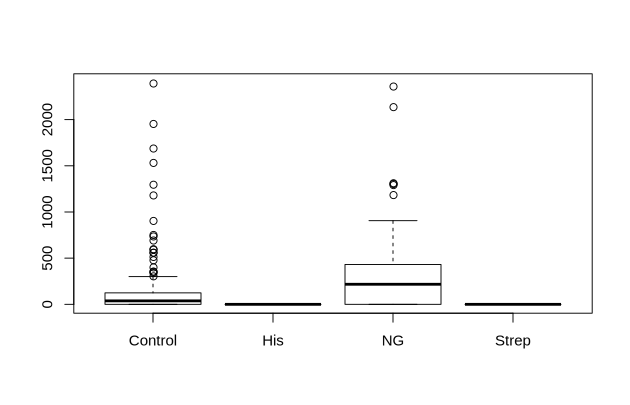
\includegraphics[width=0.6\textwidth]{Bxp.pdf}
\end{center}  

There are two immediate things to note. 
\begin{enumerate}

	\item The distributions of colony counts are very {\it skewed} --- 
	many small counts and a few large counts. We've already seen that 
	taking a log of data sometimes works in these cases. However, as the 
	tables above show, we have zero counts for all treatments and 
	$\log(0)$ is undefined. A common trick is therefore to use 
	$\log(n+1)$ (add 1 and take a log) when dealing with count data like 
	this:

\begin{lstlisting}
> colonies$logCC <- log(colonies$ColonyCount + 1)
> boxplot(logCC ~ Treatment, data=colonies)
\end{lstlisting}

\begin{center}
	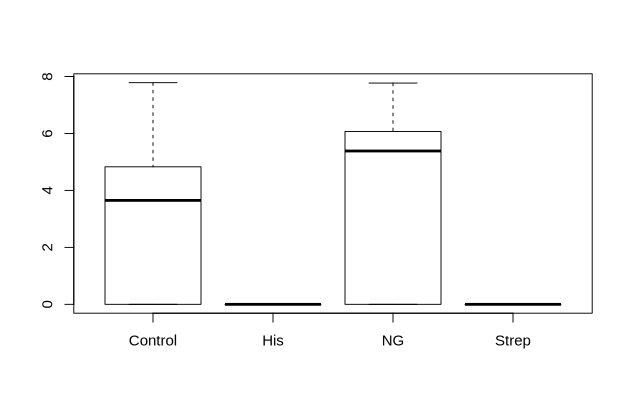
\includegraphics[width=0.6\textwidth]{logBxp.pdf} 
\end{center}

I hope you'll agree that this still doesn't look very convincingly like 
normal data, but we'll come back to this point. 

	\item The colony counts are vastly different between the different 
	treatments. It is hard to say for sure from the two plots, but it looks 
	like colonies never grow under the histidine and streptomycine 
	treatments. We can check that:

\begin{lstlisting}
> tapply(colonies$ColonyCount, colonies$Treatment, min, na.rm = TRUE)

 Control     His      NG   Strep 
       0       0       0       0 

> tapply(colonies$ColonyCount, colonies$Treatment, max, na.rm = TRUE)

 Control     His      NG   Strep 
    2400       0    2367       0 
\end{lstlisting}

There is indeed no variation at all in colony count for histidine and 
streptomycine --- colonies never grow in these treatments. We don't 
really need statistics for this observation and, in fact, variation is 
needed for statistics to work. So, for the rest of this analysis, we 
will reduce the dataset to the control and nitroguanisine treatments. 

\end{enumerate}

\begin{compactitem}[$\quad\star$]
	\item Update your script to contain the code for these plots.
\end{compactitem}

We'll use a new piece of code here to get the right subset. {\tt var 
\%in\% c('a','b','c')} finds all entries in {\tt var} whose values are 
equal to {\tt 'a'},  {\tt 'b'} or  {\tt 'c'}.

\begin{lstlisting}
> coloniesCN <- subset(colonies, Treatment %in% c("Control", "NG"), 
drop = TRUE) 
> str(coloniesCN)

 'data.frame':	340 obs. of  6 variables:
 $Student.ID : Factor w/ 34 levels "A1","A10","A11",..: 1 1 1 2 2 2 4 4 4 4 ...
 $Strain     : Factor w/ 5 levels "421","712","881",..: 4 3 5 1 2 3 4 2 3 5 ...
 $Treatment  : Factor w/ 4 levels "Control","His",..: 1 1 1 3 3 1 1 3 3 1 ...
 $ColonyCount: int  0 0 0 0 0 0 0 0 0 0 ...
 $HaloLawn   : Factor w/ 2 levels "N","Y": NA NA NA NA NA NA NA NA NA NA ...
 $logCC      : num  0 0 0 0 0 0 0 0 0 0 ...
\end{lstlisting}

You'll see that, although we have removed two treatments, their names 
still appear in the list of levels in the {\tt str} output. R retains a 
list of all the levels that were originally in a factor, even when 
those levels aren't used any more. This will be annoying later, so 
we'll use the {\tt droplevels} function to strip them out.

\begin{lstlisting}
> coloniesCN <- droplevels(coloniesCN)
> str(coloniesCN)

 'data.frame':	340 obs. of  6 variables:
 $Student.ID : Factor w/ 34 levels "A1","A10","A11",..: 1 1 1 2 2 2 4 4 4 4 ...
 $Strain     : Factor w/ 5 levels "421","712","881",..: 4 3 5 1 2 3 4 2 3 5 ...
 $Treatment  : Factor w/ 2 levels "Control","NG": 1 1 1 2 2 1 1 2 2 1 ...
 $ColonyCount: int  0 0 0 0 0 0 0 0 0 0 ...
 $HaloLawn   : Factor w/ 0 levels: NA NA NA NA NA NA NA NA NA NA ...
 $logCC      : num  0 0 0 0 0 0 0 0 0 0 ...
\end{lstlisting}

\begin{compactitem}[$\quad\star$]
	\item Add these commands to subset your data to your code file.
\end{compactitem}

\section{Looking at strains too}

Now we'll look to see how counts differ between the strains.  A simple 
way to visualise this is to use the {\tt lattice} package again to get 
plots grouped by treatment.

\begin{lstlisting}
> library(lattice) 
> bwplot(logCC ~ Strain | Treatment, data=coloniesCN)
\end{lstlisting}

\begin{center}
	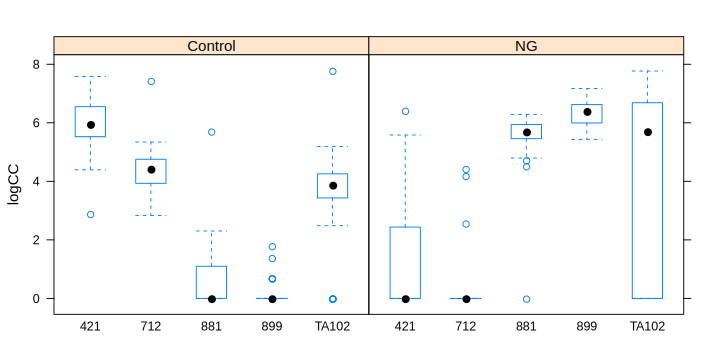
\includegraphics[width=\textwidth]{GLM_lattice.pdf}	
\end{center}

First impressions from this figure:
\begin{enumerate}
	\item The strains are doing {\it very} different things under the two 
	treatments. Hopefully this now leaps out at you as suggesting that 
	the two variables (Strain and Treatment) are {\it interacting}. \item 
	The distributions are still pretty ugly --- the variances differ 
	hugely between combinations and four combinations have a median of 
	zero.
\end{enumerate}

We could also use a barplot of means here. We'll use the original data 
to get the means, but can use a log scale on the $y$ axis ({\tt 
log='y'}).

\begin{lstlisting}
> tab <- tapply(coloniesCN$ColonyCount, list(coloniesCN$Treatment,
coloniesCN$Strain), mean, na.rm=TRUE)
> print(tab)

            421     712    881     899 TA102
 Control 538.20 138.867  12.73   0.375 126.7
 NG       61.29   5.517 292.71 593.000 523.9
\end{lstlisting}

An then, 

\begin{lstlisting}
> barplot(tab, beside=TRUE, log= ' y ' )	
\end{lstlisting}

Which should give,
\begin{center}
	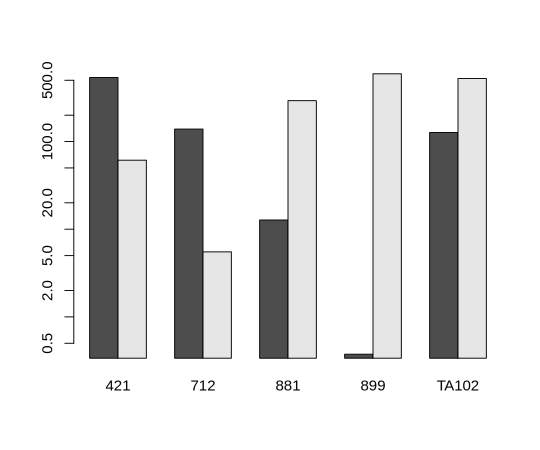
\includegraphics[width=0.6\textwidth]{GLM_barplot.pdf} 
\end{center}

Lets have a look at a first model.

\section{A linear model}

We'll fit a model of colony count as the interaction between strain and 
treatment and then look at the diagnostic plots. We'd do this anyway, 
but we're already suspicious about the variance.

\begin{lstlisting}
> modLM <- lm(logCC ~ Strain * Treatment, data=coloniesCN)
> par(mfrow=c(2,2), mar=c(3,3,3,1), mgp=c(2,0.8,0))
> plot(modLM)
\end{lstlisting}

\begin{center}
	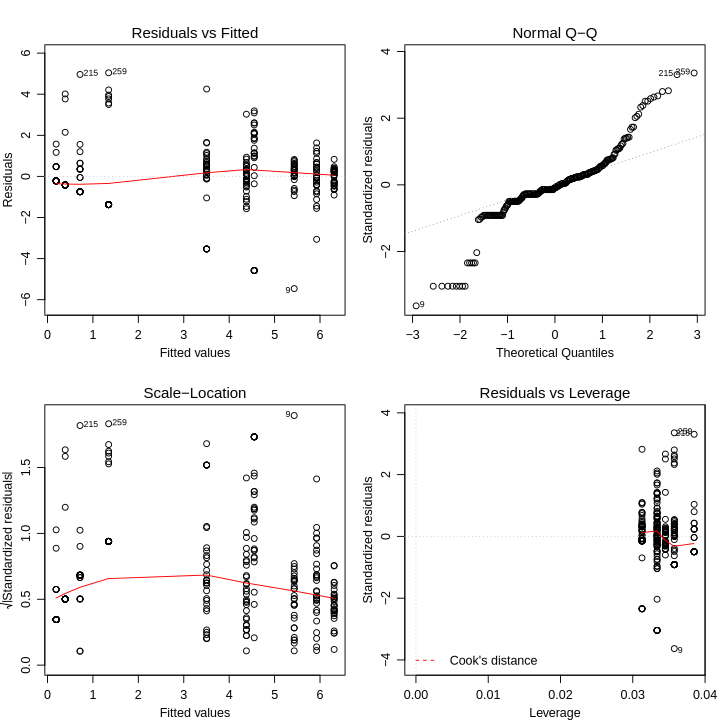
\includegraphics[width=\textwidth]{lmDisaster.pdf} 	
\end{center}

\begin{compactitem}[$\quad\star$]
	\item Run this code and have a close look at the plots. 
\end{compactitem}

That normal QQ plot is not good. Our suspicions were justified and it 
doesn't look like we can use a simple log transformation. We're not 
even going to look at the {\tt anova} and {\tt summary} tables --- if 
the diagnostic plots are bad enough, then the model outputs are not to 
be trusted.

\section{Generalised linear models}

In the linear models lecture, we looked at the expectation of {\it 
constant normal variance} in linear models. Whatever the combination of 
explanatory variables for a particular prediction, the residuals around 
that prediction have similar variance and are roughly normally 
distributed. The panel on the left shows this basic idea.

\begin{center}
	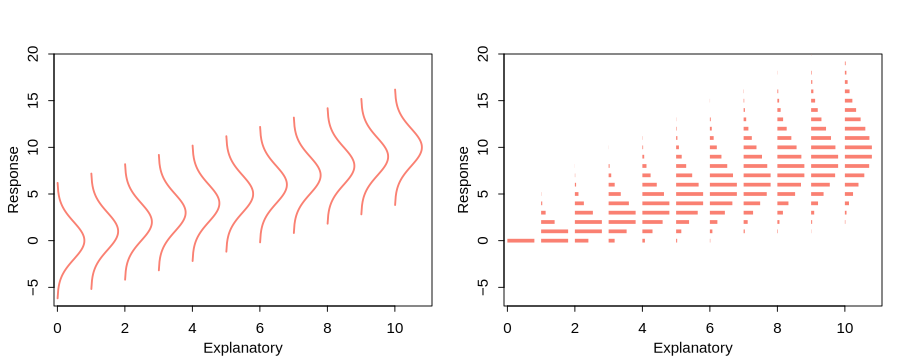
\includegraphics[width=\textwidth]{GLMexample.pdf} 
\end{center}

As we have seem, count data does not have this distribution, even when 
logged. The panel on the right shows the expected distribution of count 
data as the mean count increases with an explanatory  variable.  There 
are three key differences between the two panels:

\begin{enumerate}
	\item Counts can {\it never} be negative but can be zero.
	\item Counts are always {\it integers} --- whole numbers --- rather 
	than being continuous.
	\item The variance of count data is {\it not constant}. As the 
	average predicted count gets larger, so does the variance. Unlike the 
	normal distribution, where variance can take any value, for count 
	data  the variance is expected to be equal to the mean.
\end{enumerate}

So, we have data that is unsuitable for a linear model because it 
doesn't show constant normal variance. This is where generalised linear 
models come in --- we can change the model for the expected residuals 
to use a different distribution. For count data, this is the {\it 
Poisson} distribution.

We need to change the function we use to fit models to {\tt glm}, but 
otherwise the process is very similar. The whole point of the GLM is to 
model the original count data more appropriately, so we will abandon 
the logged data too. GLMs can cope with a range of different 
distributions, so we have to specify the {\tt family} of the 
distribution we want to use.

\begin{lstlisting}
> modPois <- glm(ColonyCount ~ Strain * Treatment, data=coloniesCN, 
family= 'poisson')
\end{lstlisting}

First, we'll look at the summary table for this model. We have 5 levels 
of strain and 2 levels of factor in the subset so we get an intercept 
($i$), 4 differences for strains($s_{2-5}$), one difference for 
treatment ($t_2$) and then four differences for the interaction 
($s_{2-5}t_2$). These combine like this:
 
\[\begin{array}{|l|c|c|}
\hline
							& \textrm{Control} & \textrm{Nitroguanisine} \\
\hline
\textrm{421}   & i        & i+t_2              \\
\textrm{712}   & i + s_2  & i+s_2+t_2+ s_2t_2  \\
\textrm{881}   & i + s_3  & i+s_3+t_2 + s_3t_2  \\
\textrm{889}   & i + s_4  & i+s_4+t_2 + s_4t_2  \\
\textrm{TA102} & i + s_5  & i+s_5+t_2  + s_5t_2 \\
\hline
\end{array}\]

The summary table looks like this --- very similar to the {\tt summary} 
table for a linear model.

\begin{lstlisting}
> summary(modPois)
 
 Call:
 glm(formula = ColonyCount ~ Strain * Treatment, family = "poisson", 
     data = coloniesCN)
 
 Deviance Residuals: 
    Min      1Q  Median      3Q     Max  
 -32.37  -10.33   -3.32    0.84   97.84  
 
 Coefficients:
                         Estimate Std. Error z value Pr(>|z|)    
 (Intercept)              6.28823    0.00787   799.0   <2e-16 ***
 Strain712               -1.35472    0.01738   -78.0   <2e-16 ***
 Strain881               -3.74421    0.05549   -67.5   <2e-16 ***
 Strain899               -7.26906    0.28878   -25.2   <2e-16 ***
 StrainTA102             -1.44651    0.01757   -82.3   <2e-16 ***
 TreatmentNG             -2.17268    0.02539   -85.6   <2e-16 ***
 Strain712:TreatmentNG   -1.05295    0.08446   -12.5   <2e-16 ***
 Strain881:TreatmentNG    5.30786    0.06152    86.3   <2e-16 ***
 Strain899:TreatmentNG    9.53871    0.28989    32.9   <2e-16 ***
 StrainTA102:TreatmentNG  3.59226    0.03090   116.2   <2e-16 ***
 ---
 Signif. codes:  0 '***' 0.001 '**' 0.01 '*' 0.05 '.' 0.1 ' ' 1 
 
 (Dispersion parameter for poisson family taken to be 1)
 
     Null deviance: 134445  on 293  degrees of freedom
 Residual deviance:  61579  on 284  degrees of freedom
   (46 observations deleted due to missingness)
 AIC: 62910
 
 Number of Fisher Scoring iterations: 7
 
\end{lstlisting}

So, interpreting this table quickly. Under the control treatment, 
strain 421 (the intercept) has the highest number of colonies and all 
the other strains have lower numbers to some degree --- the differences 
are negative. The overall effect of nitrogaunasine is to decrease the 
number of colonies --- again a negative coefficient --- but then the 
positive interactions show big increases in colony counts for 
nitroguanisine for specific strains. Everything is hugely significant.

\begin{compactitem}[$\quad\star$]
	\item Copy the code in this section into your script and explore the 
	model.
\end{compactitem}

\section{Overdispersion}

There's a problem. You may have already spotted it:

\begin{lstlisting}
> par(mfrow = c(2, 2), mar = c(3, 3, 3, 1), mgp = c(2, 0.8, 0))
> plot(modPois)
\end{lstlisting}

\begin{center}
	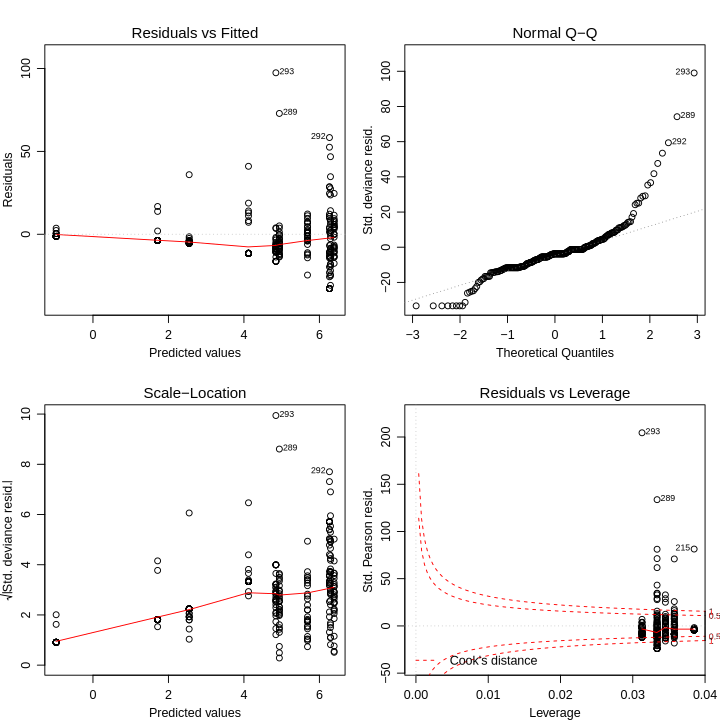
\includegraphics[width=0.8\textwidth]{poisDiag.pdf}
\end{center}

Actually, there are two problems. First, that QQ plot is still a bit 
dubious. More of the points are close to the line than in the linear 
model but there are some extreme positive residuals. Second, the 
magnitude of the residuals is enormous, and this is really clear in the 
plot in the bottom right hand corner. This plot identifies outliers and 
any points outside of the red dotted line are possible problems.

The problem here is {\it overdispersion}. The Poisson distribution 
predicts that the variance at a point in the model is equal to the 
prediction --- the mean count at that point. Our count data shows much 
more variance than this --- particularly that there are some huge 
counts given the means.

There is a simple way to check the dispersion of count data using the 
{\tt summary} table: the ratio of the residual deviance to the residual 
degrees of freedom should be approximately 1. This expectation is 
actually given in the table:

{\tt (Dispersion parameter for poisson family taken to be 1)}

In this case,  the ratio is $61579/284=216.8$. That's very strongly 
overdispersed. Fortunately, we can allow for this by using a different 
model.

\section{Generalised linear models using quasipoisson}

The quasipoisson family uses the data to estimate the dispersion of the 
model, but is otherwise very similar to using the Poisson family.

\begin{lstlisting}
> modQPois <- glm(ColonyCount ~ Strain * Treatment, data=coloniesCN,
family= 'quasipoisson')
\end{lstlisting}

The summary table now looks like this:

\begin{lstlisting}
> summary(modQPois) 

 Call:
 glm(formula = ColonyCount ~ Strain * Treatment, family = "quasipoisson", 
     data = coloniesCN)
 
 Deviance Residuals: 
    Min      1Q  Median      3Q     Max  
 -32.37  -10.33   -3.32    0.84   97.84  
 
 Coefficients:
                         Estimate Std. Error t value Pr(>|t|)    
 (Intercept)                6.288      0.158   39.78  < 2e-16 ***
 Strain712                 -1.355      0.349   -3.88  0.00013 ***
 Strain881                 -3.744      1.115   -3.36  0.00089 ***
 Strain899                 -7.269      5.800   -1.25  0.21113    
 StrainTA102               -1.447      0.353   -4.10  5.4e-05 ***
 TreatmentNG               -2.173      0.510   -4.26  2.8e-05 ***
 Strain712:TreatmentNG     -1.053      1.696   -0.62  0.53529    
 Strain881:TreatmentNG      5.308      1.236    4.30  2.4e-05 ***
 Strain899:TreatmentNG      9.539      5.822    1.64  0.10246    
 StrainTA102:TreatmentNG    3.592      0.621    5.79  1.9e-08 ***
 ---
 Signif. codes:  0 '***' 0.001 '**' 0.01 '*' 0.05 '.' 0.1 ' ' 1 
 
 (Dispersion parameter for quasipoisson family taken to be 403.4)
 
     Null deviance: 134445  on 293  degrees of freedom
 Residual deviance:  61579  on 284  degrees of freedom
   (46 observations deleted due to missingness)
 AIC: NA
 
 Number of Fisher Scoring iterations: 7 
\end{lstlisting}

This is pretty similar to the previous table but there two differences. 
First, the dispersion parameter line has changed. Second, all the $p$ 
values have got less significant -- this is the effect of controlling 
for the overdispersion. 

We'll look at the model diagnostic plots next:

\begin{lstlisting}
> par(mfrow = c(2, 2), mar = c(3, 3, 3, 1), mgp = c(2, 0.8, 0))
> plot(modQPois)	
\end{lstlisting}

\begin{center}
	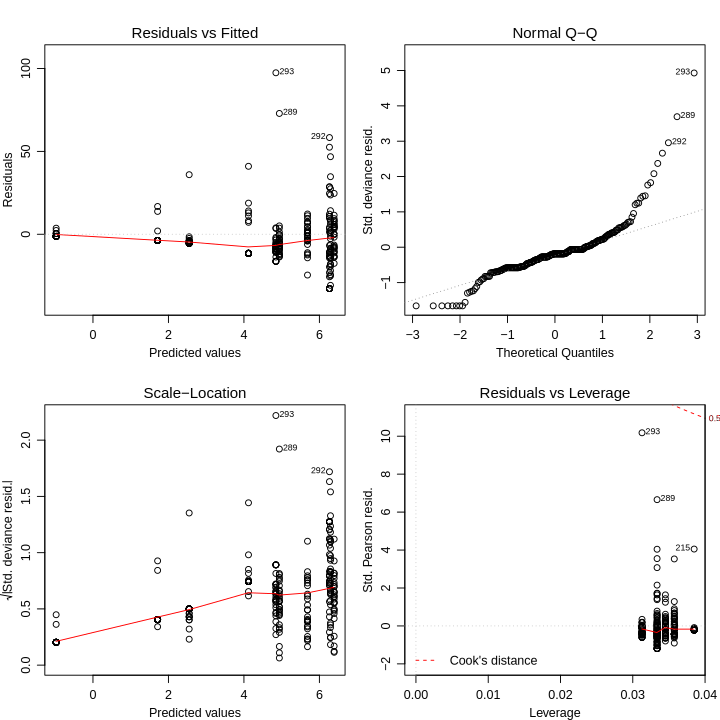
\includegraphics[width=0.8\textwidth]{qpoisDiag.pdf} 
\end{center}

The residuals and leverage plot is now ok. The QQ plot is not better, 
but is still an improvement over the original linear model. We can't 
improve the model fit any more ---  it isn't perfect but we'll accept 
those imperfections. It is worth thinking about the imperfections 
though --- what might give rise to occasional larger than expected 
counts of colonies?

We'll look at the {\tt anova} table next. Technically, this is now 
analysis of deviance not analysis of variance but the concept is the 
same. Different tests are appropriate for different families of 
distribution, but we can use $F$ here:

\begin{lstlisting}
> anova(modQPois, test = "F")

 Analysis of Deviance Table
 
 Model: quasipoisson, link: log
 
 Response: ColonyCount
 
 Terms added sequentially (first to last)
 
 
                  Df Deviance Resid. Df Resid. Dev     F  Pr(>F)    
 NULL                               293     134445                  
 Strain            4    13923       289     120521  8.63 1.4e-06 ***
 Treatment         1     6055       288     114467 15.01 0.00013 ***
 Strain:Treatment  4    52888       284      61579 32.78 < 2e-16 ***
 ---
 Signif. codes:  0 '***' 0.001 '**' 0.01 '*' 0.05 '.' 0.1 ' ' 1 
\end{lstlisting}

Can we simplify the model? The interaction is the only term we can drop 
and looks highly significant, but we can check by deleting it.

\begin{lstlisting}
> drop.scope(modQPois)

 [1] "Strain:Treatment"

> modQPois2 <- update(modQPois, . ~ . - Strain:Treatment)
> anova(modQPois, modQPois2, test = "F")

 Analysis of Deviance Table
 
 Model 1: ColonyCount ~ Strain * Treatment
 Model 2: ColonyCount ~ Strain + Treatment
   Resid. Df Resid. Dev Df Deviance    F Pr(>F)    
 1       284      61579                            
 2       288     114467 -4   -52888 32.8 <2e-16 ***
 ---
 Signif. codes:  0 '***' 0.001 '**' 0.01 '*' 0.05 '.' 0.1 ' ' 1 
\end{lstlisting}

No, that makes the model much worse, so we now have our final model. 

\begin{compactitem}[$\quad\star$]
	\item Fit this new model in your script and check you've got the same 
	results.
\end{compactitem}

\section{Model predictions}

We can get model predictions and standard errors using the {\tt 
predict} function. There is a difference though. GLMs use an internal 
transformation to model the data using a {\it link function} and the 
coefficients in the summary above are on the scale of the link 
transformation. For quasipoisson, this is a {\it log link}, which you 
can see in the output of {\tt anova}. You can use {\tt predict} to get 
predictions on the scale of the original {\it response}.

\begin{lstlisting}
# use expand.grid to get all combinations of factors
> df <- expand.grid(Strain = levels(coloniesCN$Strain), Treatment =
levels(coloniesCN$Treatment))
> predict(modQPois, newdata = df, type = "response")

       1       2       3       4       5       6       7       8       9      10 
 538.200 138.867  12.731   0.375 126.687  61.286   5.517 292.714 593.000 523.900 
\end{lstlisting}

Those are the same values as the means we calculated for the barplot. 
Adding standard errors to barplots is more difficult for GLMs and we 
won't go into it here.

\section{Reporting the model}

Reporting complicated statistics is a difficult business. There is a 
lot of detail involved and you want the reader to understand what you 
have done well enough to repeat the analysis if needed. You also have 
to summarise and explain the results without pages of R output. 

Here are some pointers:
\begin{itemize}
	\item What does the data show? Present a graph or a table to show the 
	data you are about to model. {\it Always} include a figure or table 
	legend and {\it always} refer to that figure or legend from the text.
	\item Have you transformed the data or used a subset? If so, why?
	\item What kind of model or statistical test have you used?
	\item With linear models, what is the response variable and what are 
	the explanatory variables.
	\item Have you simplified the model and, if so, what was the most 
	complex model you tried?
	\item How did you check the suitability of the model? Are there any 
	problems with the model and, if so, what might cause them?
	\item If you summarise stats in text, you must include all the 
	information about the test. 
	\begin{itemize}
		\item For $F$ tests, this is $F$, the two degrees of freedom and 
		the p value. For example: `There is a significant interaction 
		between treatment and strain ($F_{4,284}=32.7, p < 0.0001$)'. 
		\item For $t$ tests, this is the coefficient, the standard error, 
		$t$, the degrees of freedom and $p$. For example, `Across strains, 
		the main effect of nitroguanisine is to reduce colony counts 
		relative to the control (estimate=-2.17, s.e= 0.51, $t=-4.26$, 
		df=284,  $p < 0.0001$)'.
	\end{itemize}
	\item With more complex models, it is common to present either the 
	anova table or the coefficients table as a summary of the model 
	output. Just include the tables from R output, not the information 
	around it. See Table 1 for an example. 
	\item {\it Never} just include chunks of raw output from R.
	\item Most importantly, what is the interpretation of the model. What 
	is it telling you about the data?
\end{itemize}

{\it Table 1}: Coefficients from a GLM of treatment and strain as 
predictors of colony count.

% latex table generated in R 2.14.1 by xtable 1.7-0 package
% Wed Nov 28 08:56:01 2012
\begin{table}[ht]
	\begin{center}
		\begin{tabular}{rrrrl}
		  \hline
		 & Estimate & Std. Error & t value & p \\ 
		  \hline
		(Intercept) & 6.29 & 0.16 & 39.78 & <0.0001 \\ 
		  Strain712 & -1.35 & 0.35 & -3.88 & \phantom{<}0.0001 \\ 
		  Strain881 & -3.74 & 1.11 & -3.36 & \phantom{<}0.0009 \\ 
		  Strain899 & -7.27 & 5.80 & -1.25 & \phantom{<}0.2111 \\ 
		  StrainTA102 & -1.45 & 0.35 & -4.10 & <0.0001 \\ 
		  TreatmentNG & -2.17 & 0.51 & -4.26 & <0.0001 \\ 
		  Strain712:TreatmentNG & -1.05 & 1.70 & -0.62 & \phantom{<}0.5353 \\ 
		  Strain881:TreatmentNG & 5.31 & 1.24 & 4.30 & <0.0001 \\ 
		  Strain899:TreatmentNG & 9.54 & 5.82 & 1.64 & \phantom{<}0.1025 \\ 
		  StrainTA102:TreatmentNG & 3.59 & 0.62 & 5.79 & <0.0001 \\ 
		   \hline
		\end{tabular}
	\end{center}
\end{table}

\section{Halos and lawns}

We'll keep this one simple since it is harder to analyse. The response 
variable ({\tt HaloLawn}) is binary --- the plates either have a lawn 
or not. We'll just look at a contingency table of how many plates have 
halos or lawns under each combination of treatment and strain.

\begin{lstlisting}

> table(Halo = colonies$HaloLawn, Strain = colonies$Strain, Treatment = 
colonies$Treatment)

 , , Treatment = Control
 
     Strain
 Halo 421 712 881 899 TA102
    N   0   0   0   0     0
    Y   0   0   0   0     0
 
 , , Treatment = His
 
     Strain
 Halo 421 712 881 899 TA102
    N   1   1   0   0     1
    Y  29  29  26  32    31
 
 , , Treatment = NG
 
     Strain
 Halo 421 712 881 899 TA102
    N   0   0   0   0     0
    Y   0   0   0   0     0
 
 , , Treatment = Strep
 
     Strain
 Halo 421 712 881 899 TA102
    N   5  30   5  21     0
    Y  25   0  25   9    32
 
\end{lstlisting}

So, lawns and halos are never recorded from nitroguanisine or the 
control. They're nearly always found with histidine and different 
strains have different response to streptomysin. Again, treatment and 
strain interact. Although you can use a $\chi^2$ test with two 
dimensional contingency tables to look for independence between 
factors, you can't with a three-way table. 
 % glm}
 
 % 
 
% \backmatter%%%%%%%%%%%%%%%%%%%%%%%%%%%%%%%%%%%%%%%%%%%%%%%%%%%%%%%

%%%%%%%%%%%%%%%%%%%%%%%%%%%%%%%%%%%%%%%%%%%%%%%%%%%%%%%%%%%%%%%%%%%%%%

\end{document}
